\startchapter{Analysis}
\label{chapter:analysis}
After data and simulated data samples are produced and physics objects are defined and reconstructed within them, the resulting information can be analyzed to search for evidence of the existence of new physics.

This thesis focuses on the design of the most sensitive ``merged" signal region as well as the addition of a control region to constrain the \ttbar background contribution. Other analysis regions are described in more brief detail in order to provide context to decision-making and a fuller picture of the analysis.

\section{Cut and Count Analysis}
This analysis uses the ``cut and count" strategy to search for evidence of the signal model. In a cut and count analysis a set of selection criteria are chosen which slice or ``cut" the data according to various event variables, such as the amount of missing transverse momentum. These selection criteria are chosen in order to maximize the expected number of signal events and minimize the expected number of standard model background events entering the region based on the MC simulated data. While designing the selection criteria, real ATLAS data is blinded to avoid biasing the selection. The final area of phase space defined by the selection criteria is known as the ``signal region". At the culmination of an analysis, the real ATLAS data can be compared with the simulated MC data and a statistical conclusion can be reached about the likelihood of the existence of the signal model.

In order to improve the accuracy and uncertainty of the predicted standard model background a ``control region" may also be used. This is a region orthogonal to the signal region which is designed to have similar kinematic properties but be more pure in one or more standard model backgrounds and much less rich in expected signal events. In this region the number of MC simulated background events and ATLAS data events are compared. Their ratio can therefore provide additional information to correct and constrain the expected number of background events in the signal region.

\section{Analysis Strategy}
\label{section:ana_strat}
In this analysis there are two analysis channels which are combined statistically during fitting. These channels are distinguished by the reconstruction of the dijet system from the hadronically decaying W boson, and are named the \merged channel and the \resolved channel. In the \merged channel the dijet system is reconstructed by a single $R=1.0$ TAR jet, which generally means it is more boosted with the $s$ decay products closer together. In the less-boosted \resolved channel the dijet system is reconstructed by a pair of $R=0.4$ jets. Figure \ref{fig:mgd_res} provides a visual demonstration of this difference. In each analysis channel there are three analysis regions: the semileptonic signal region, a control region designed to constrain the \ttbar background, and a control region designed to constrain the \wjets background. To ensure \merged and \resolved regions are orthogonal, an event recycling strategy is employed where only events failing the selection for all \merged regions are considered for selection in \resolved regions.

\begin{figure}[h!]
    \centering
    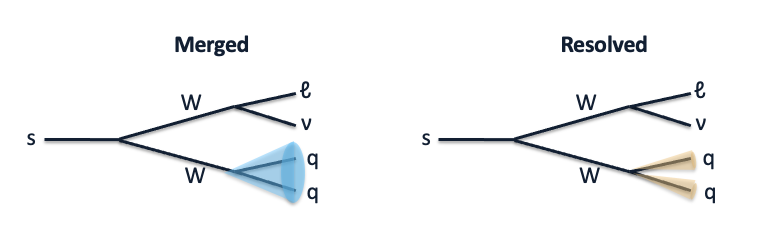
\includegraphics[width=0.8\textwidth]{Figures/4/mgd_res.png}
    \caption{Schematic representation of the differing reconstruction technique between merged and resolved regions.}
    \label{fig:mgd_res}
\end{figure}

\section{Merged Signal Region}
Something here??
\label{section:sr_merged}
\subsection{Signal and Background Characterization}
The first step towards defining signal region selection criteria was to characterize the signal and background events while searching for exploitable differences. Event characteristics explored include the relative positions of analysis objects, the transverse momenta and masses of analysis objects, along with various jet substructure variables. Figure ~ in \ref{chapter:appendix}

\subsection{TAR Jet Lepton Disentanglement}
Reconstructing the hadronically decaying W-boson as accurately as possible is key in this analysis. As a result, it was given special attention, especially in the more sensitive merged channel. In this channel, the W is reconstructed by a single $R=1.0$ TAR jet. Due to the boosted nature of the $s$-decay, however, the leptonically decaying W often lies very near to this jet. As a result the lepton often overlaps the TAR jet, which can lead to difficulty in jet reconstruction.

In order to resolve this difficulty, modifications are made to the TAR jet building process to disentangle overlapping leptons. Input tracks and jets that are considered likely to be attributable to a final state lepton and not the hadronic W decay are removed. First, tracks associated with a baseline electron or muon are removed from the input track collection. Additionally, any \akt $R=0.2$ jet overlapping with a baseline electron (defined here as having $\Delta R(lep,jet) < 0.2$) is removed prior to reclustering into $R=1.0$ jets. $R=0.2$ jets overlapping muons are not removed, as muons do not leave a calorimeter signature and are therefore unlikely to fake hadronic activity. This results in the following updated TAR jet building algorithm, where steps with a (*) are added to disentangle leptons:

\begin{itemize}
  \item Tracks and calibrated \akt $R=0.2$ jets are chosen as input to the algorithm.
  \item Tracks associated with a baseline muon or electron are removed from the input collection (*).
  \item \akt $R=0.2$ jets overlapping with a baseline electron ($\Delta R<0.2$) are removed from the input collection (*).
  \item The remaining \akt $R=0.2$ jets are reclustered using the \akt algorithm into $R=1.0$ jets and trimmed using the $p_T$ fraction \(f_{cut}=0.05\).
  \item Input tracks are matched to $R=0.2$ jets if possible using ghost association.
  \item Tracks which remain unassociated are matched to the nearest \akt $R=0.2$ jet within $\Delta R<0.3$
  \item The \pT of each track is rescaled using the \pT of the jet to which it is matched using the equation:
  \begin{equation}
  \pT^{\text{track, new}} = \pT^{\text{track, old}}\times \frac{\pT^{\text{subjet $j$}}}{\sum_{i \in j} \pT^{\text{track $i$}}} ,
  \label{eq:TAR_rescale}
  \end{equation}  where $j$ is the $R=0.2$ subjet that the track being rescaled is matched with, and the index $i$ runs over all tracks matched to that subjet. This rescaling accounts for the missing neutral momentum, which is measured at calorimeter level but is not present at tracker level.
  \item Finally, jet substructure variables and  $m^\text{TAR}$ are calculated using the rescaled matched tracks.
\end{itemize}

In order to study the potential benefit of lepton-disentanglement, near-identical ntuples of signal MC samples were produced with one implementing disentanglement and the other not.
The mass of the reconstructed jets in the two samples were then compared in a region where an electron overlaps the $R=1.0$ TAR Jet $(\Delta R(e, $R=1.0$ TAR) < 1)$, to determine how well the $W$ boson mass is reconstructed in this case.
Figure \ref{fig:TARdisentaglementplots} demonstrates the improvement in mass resolution achieved by disentangling leptons from TAR jets. A clearly enhanced resolution in the TAR jet mass peak around the $W$ mass is visible for the disentangled jets. This significantly improves sensitivity in the merged electron signal region.

\begin{figure}[!h]
\centering
   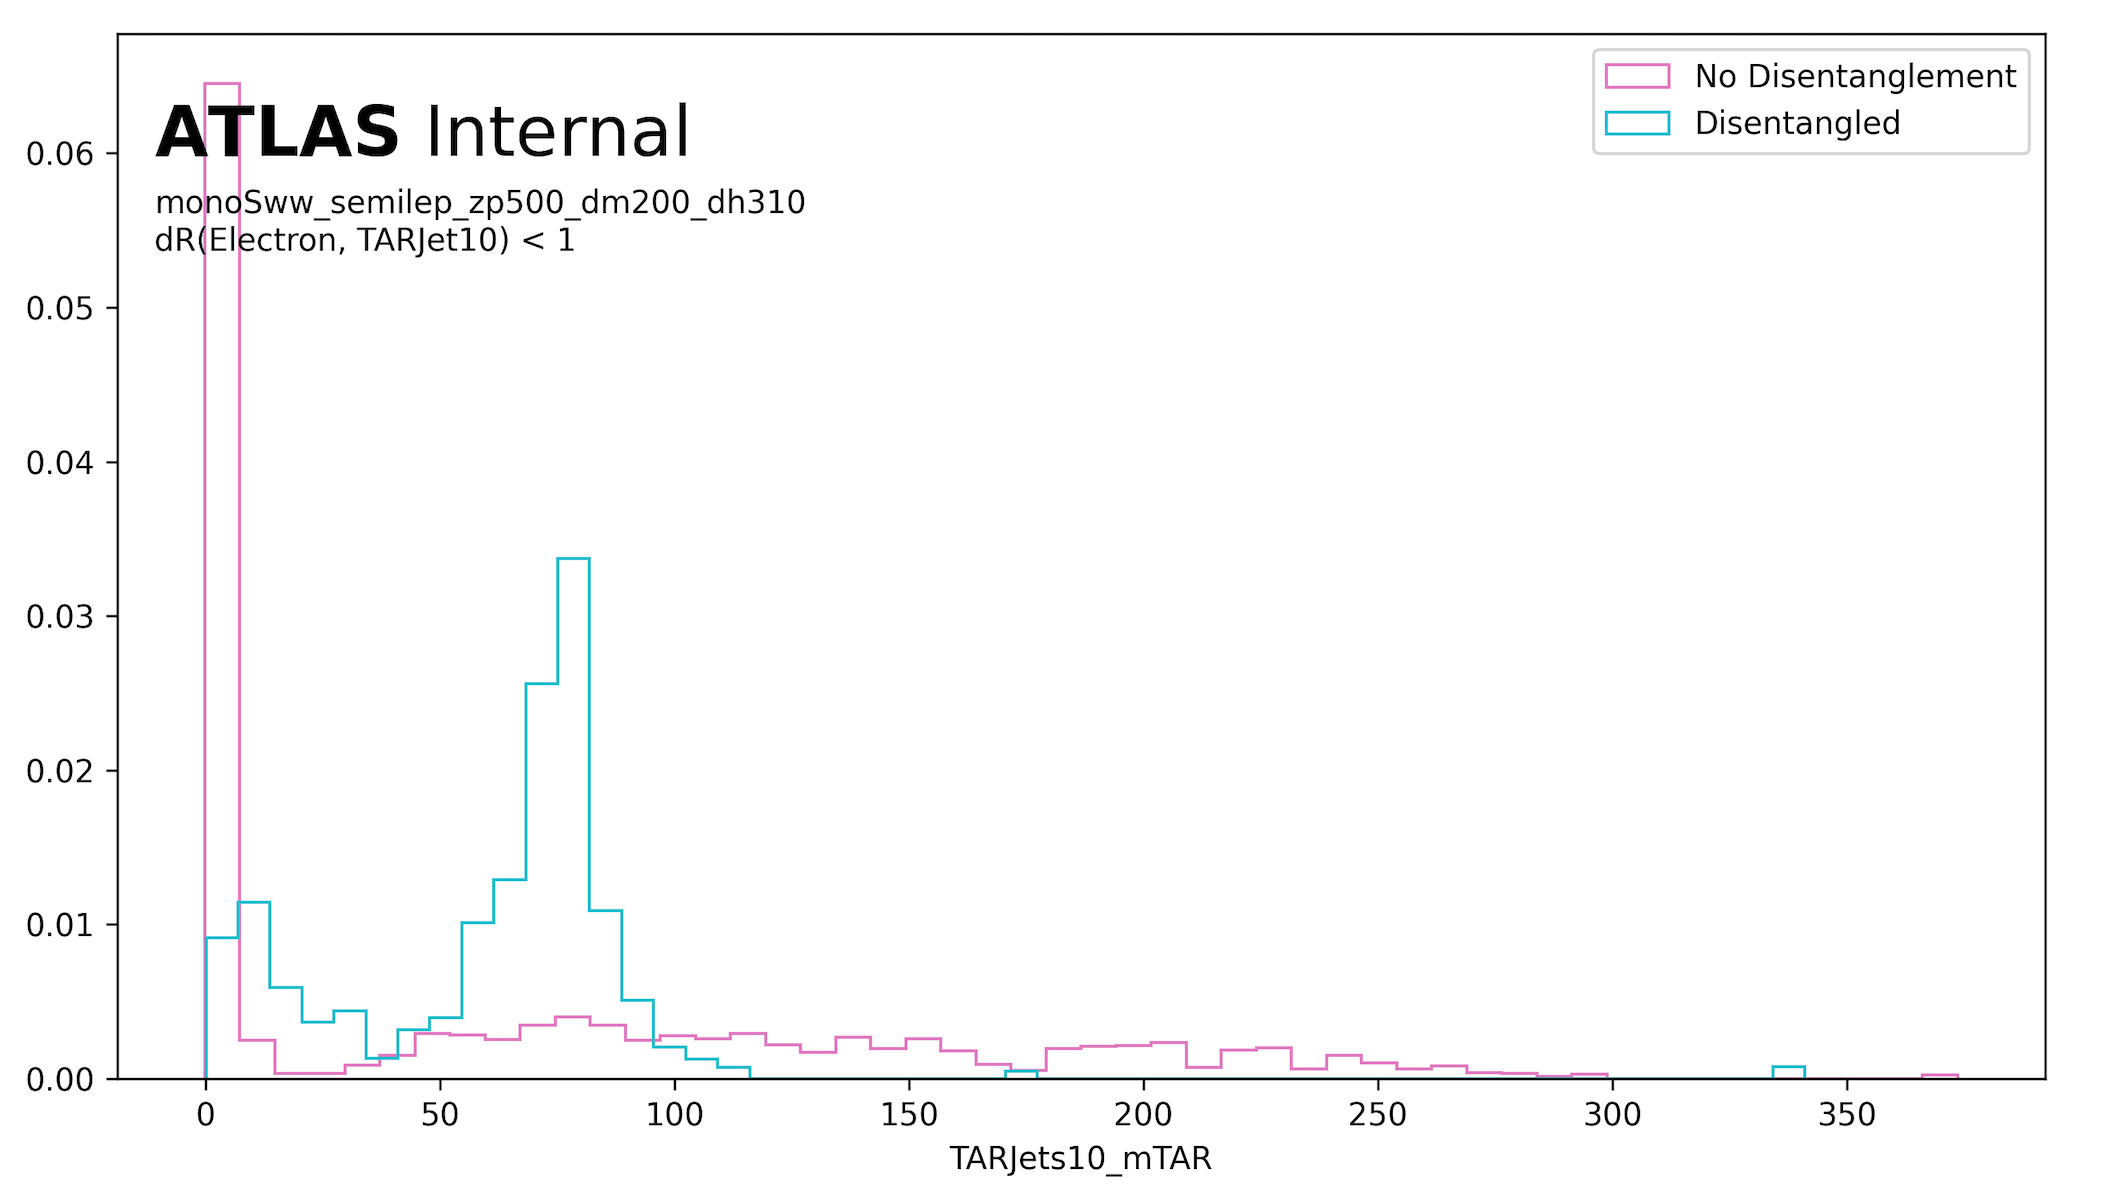
\includegraphics[width = 0.49\textwidth]{Figures/4/TAR/monoSww_semilep_zp500_dm200_dh310.png}
   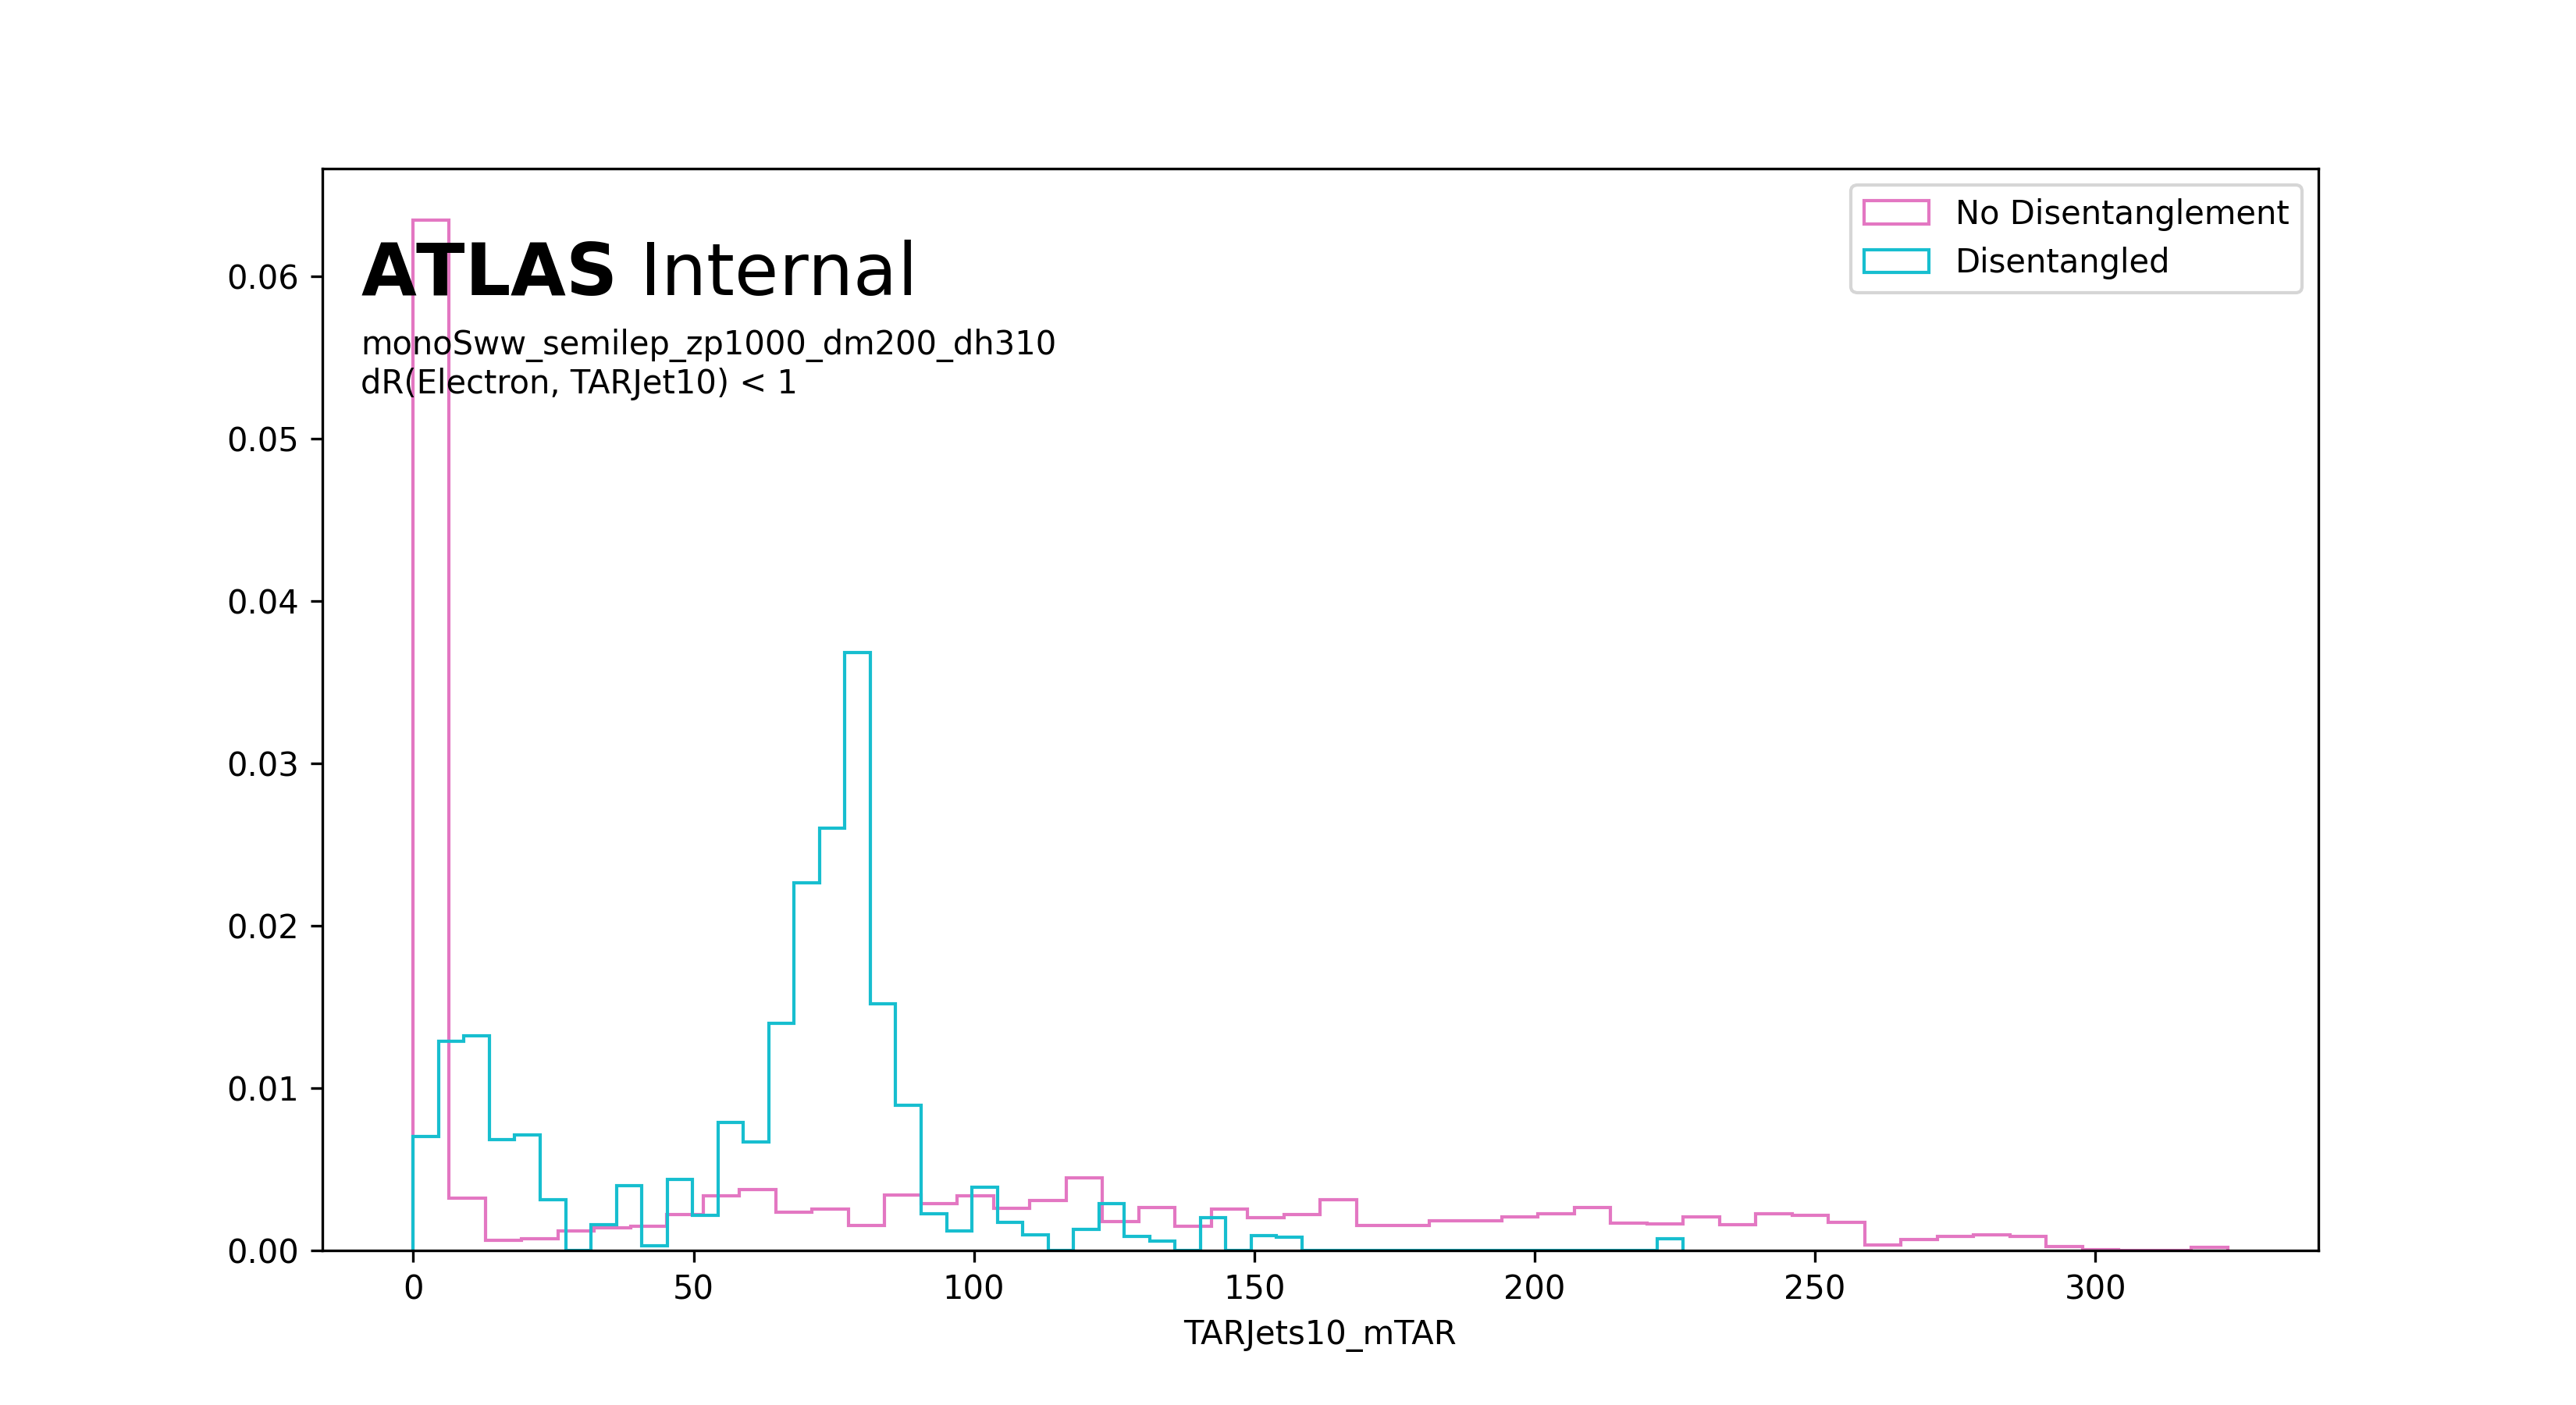
\includegraphics[width = 0.49\textwidth]{Figures/4/TAR/monoSww_semilep_zp1000_dm200_dh310.png}

   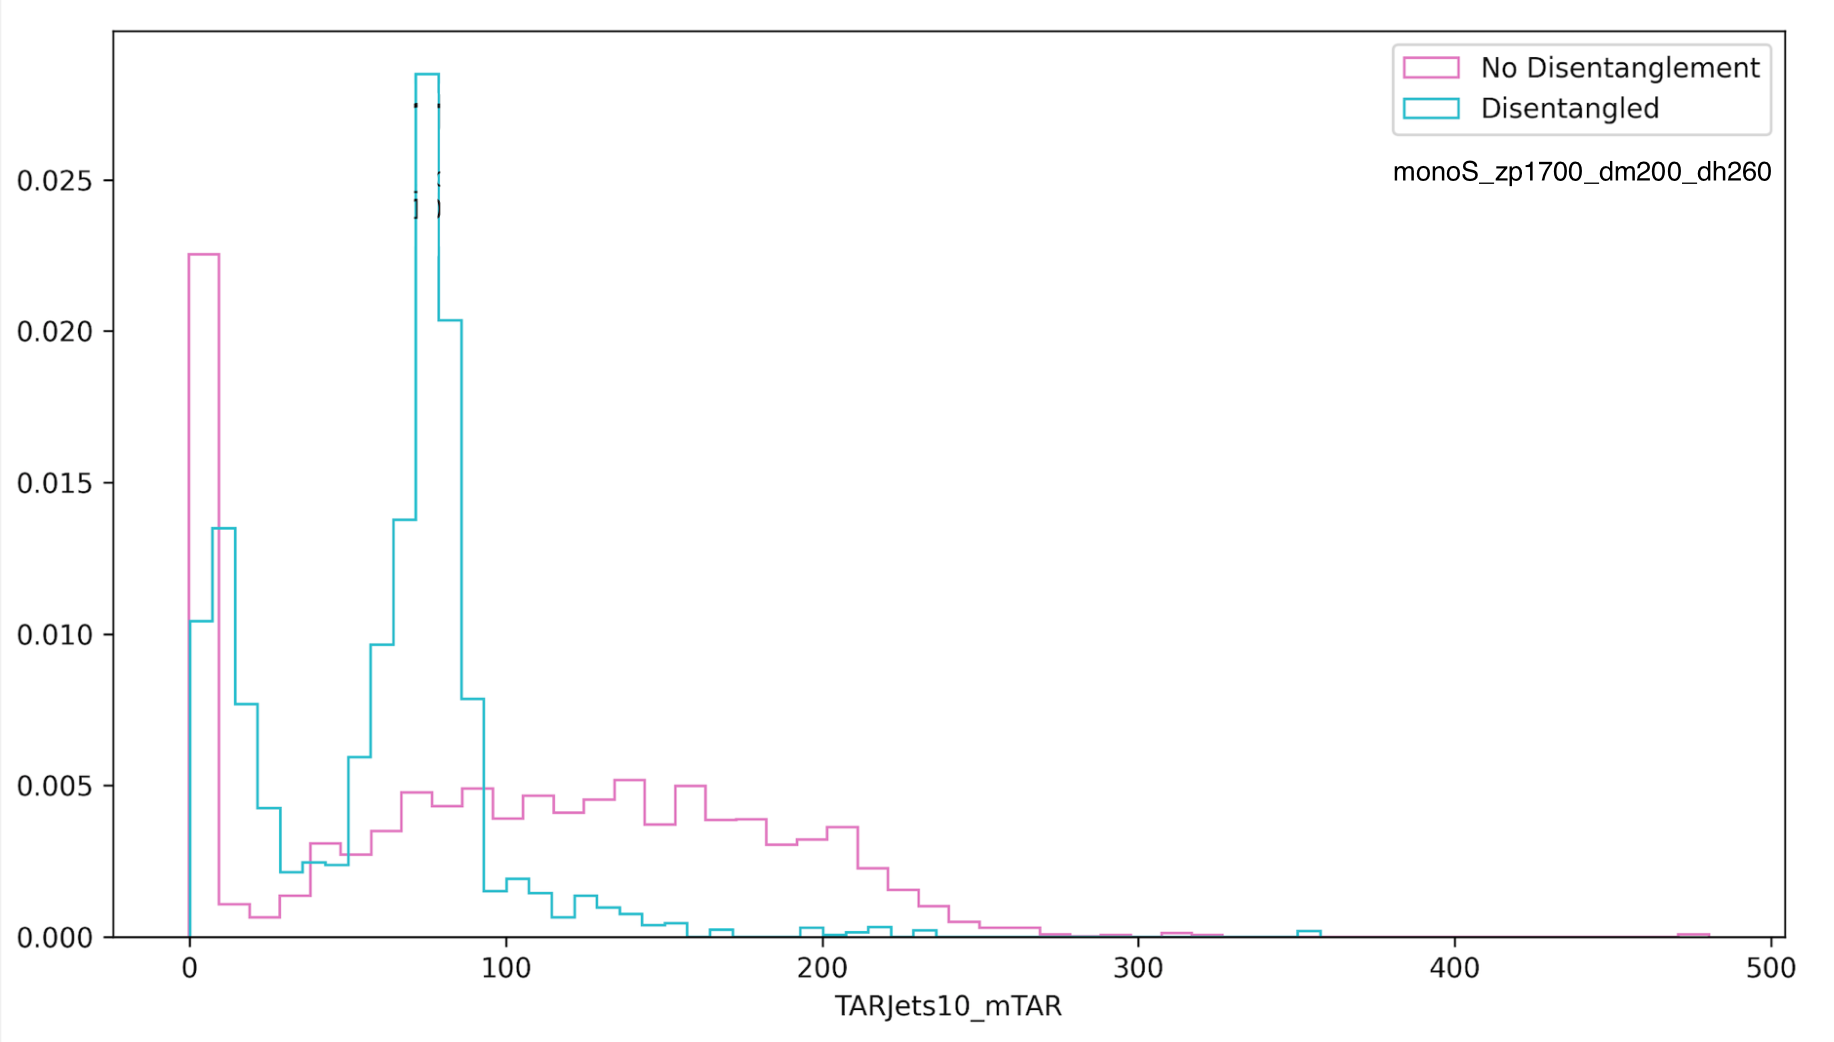
\includegraphics[width = 0.49\textwidth]{Figures/4/TAR/monoSww_semilep_zp1700_dm200_dh260.png}
   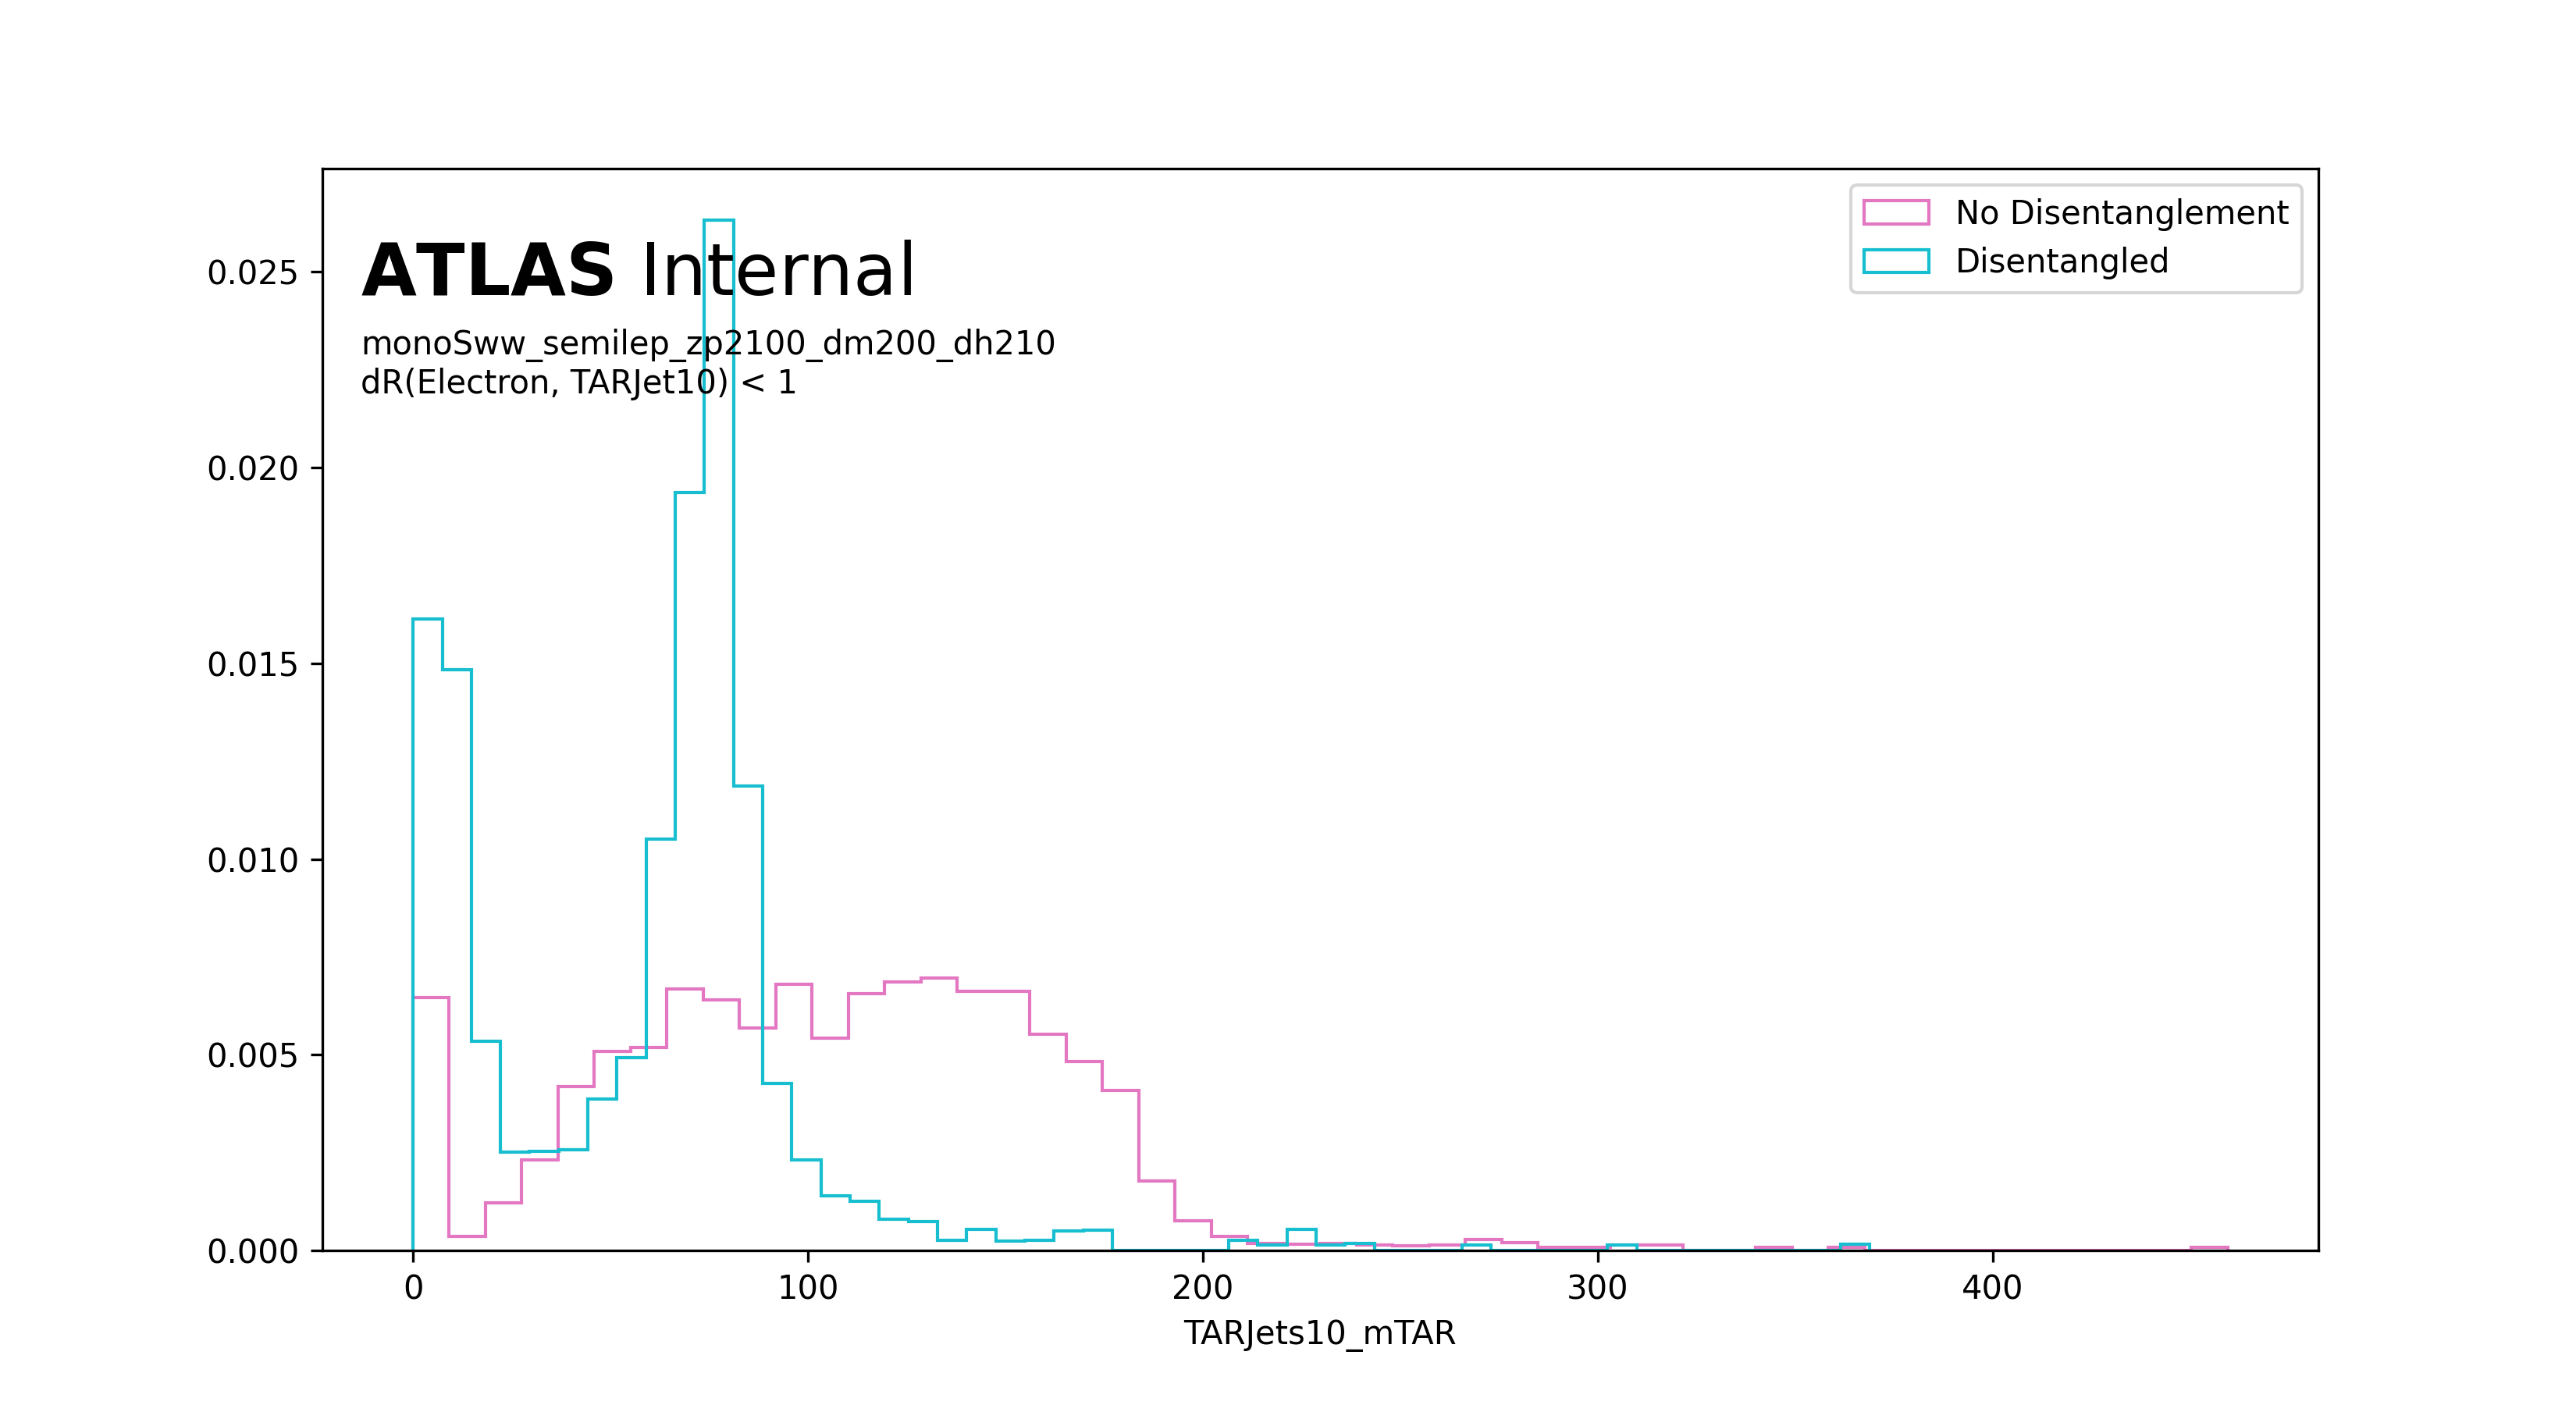
\includegraphics[width = 0.49\textwidth]{Figures/4/TAR/monoSww_semilep_zp2100_dm200_dh210.png}

   \caption{Normalized $R=1.0$ TAR jet mass distributions with and without lepton disentanglement applied for several representative signal points}
   \label{fig:TARdisentaglementplots}
\end{figure}


An additional study was undertaken to compare the performance of building the TAR jets from constituent \akt $R=0.4$ jets rather than \akt $R=0.2$ jets.
In the electron region it was found that for high $s$ mass, $W$ mass resolution performance was similar between the two methods, but for low $s$ mass, using \akt $R=0.4$ jets significantly resolution around the $W$ mass.
In the muon region few significant differences were observed.
Figure \ref{fig:R04_TAR_plots} shows a comparison of the TAR jet mass distribution built from \akt $R=0.4$ and \akt $R=0.2$ for select signal points in a signal enriched region with 1 electron and \Delta R(e, $R=1.0$ TAR)$< 1$ and $\mtlepmet > 150$ \GeV.

\begin{figure}[htpb]
  \centering
     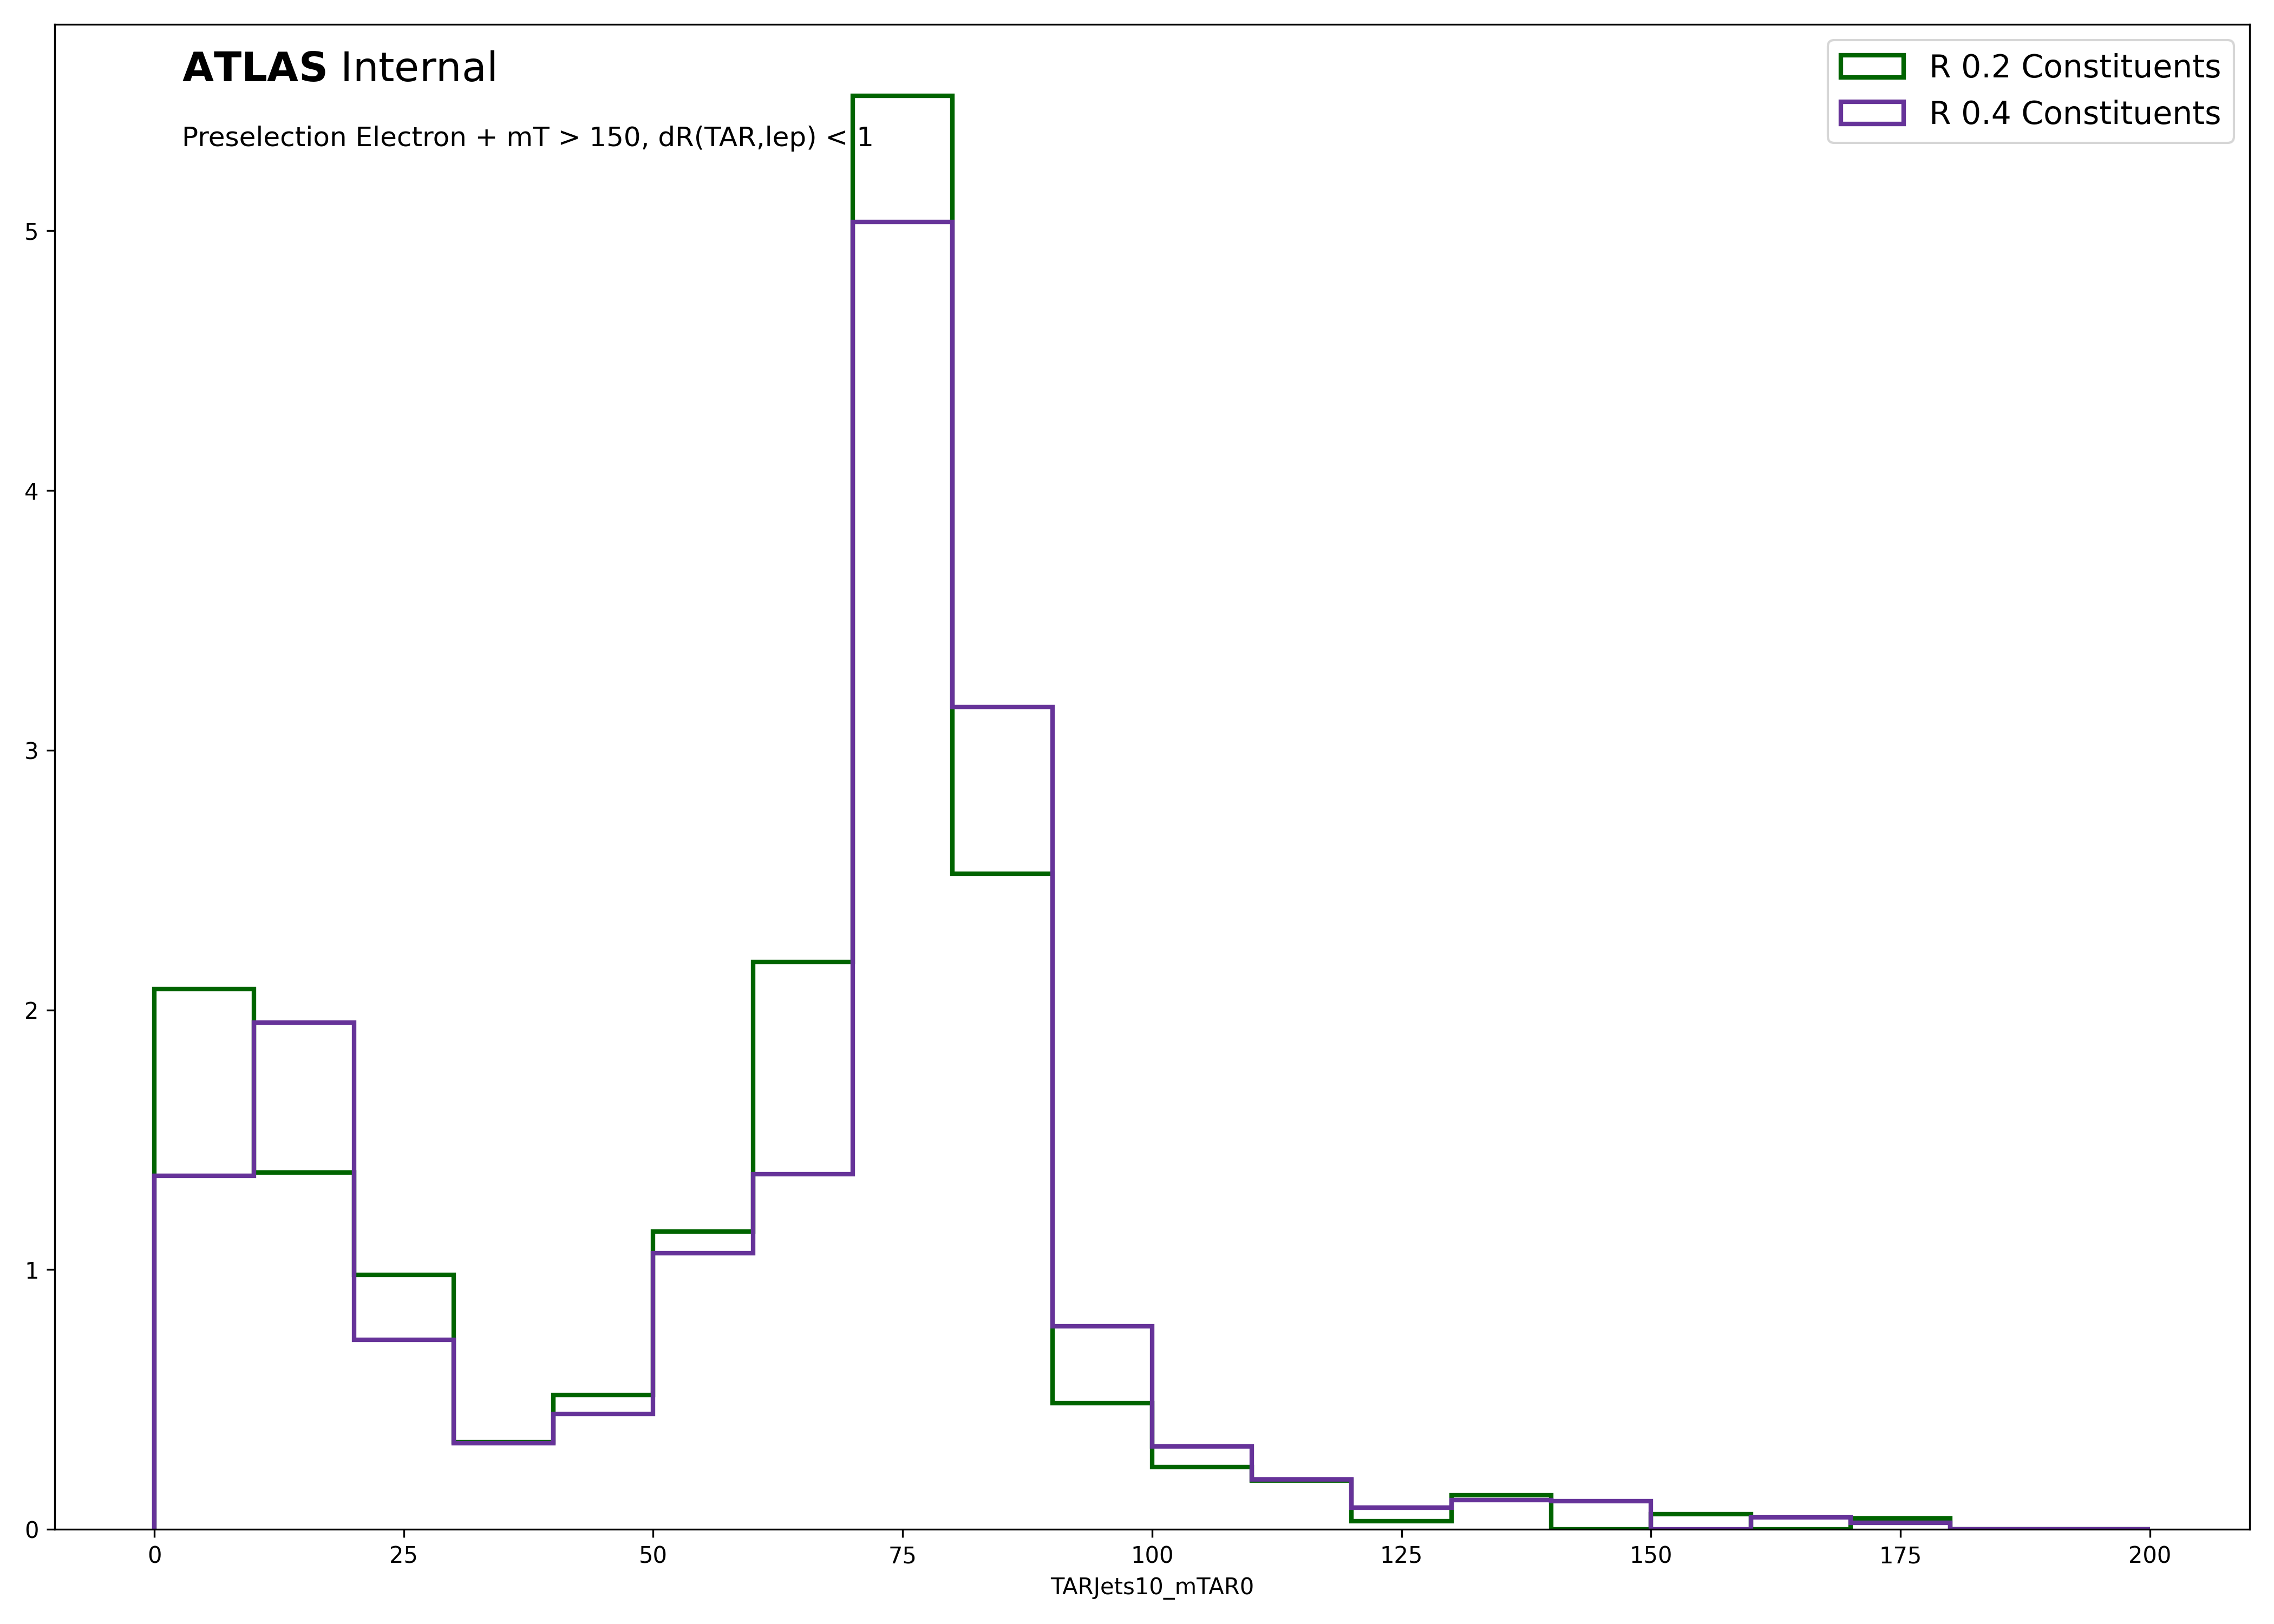
\includegraphics[width = 0.49\textwidth]{Figures/4/TAR/04_monoSww_semilep_zp500_dm200_dh310.png}
     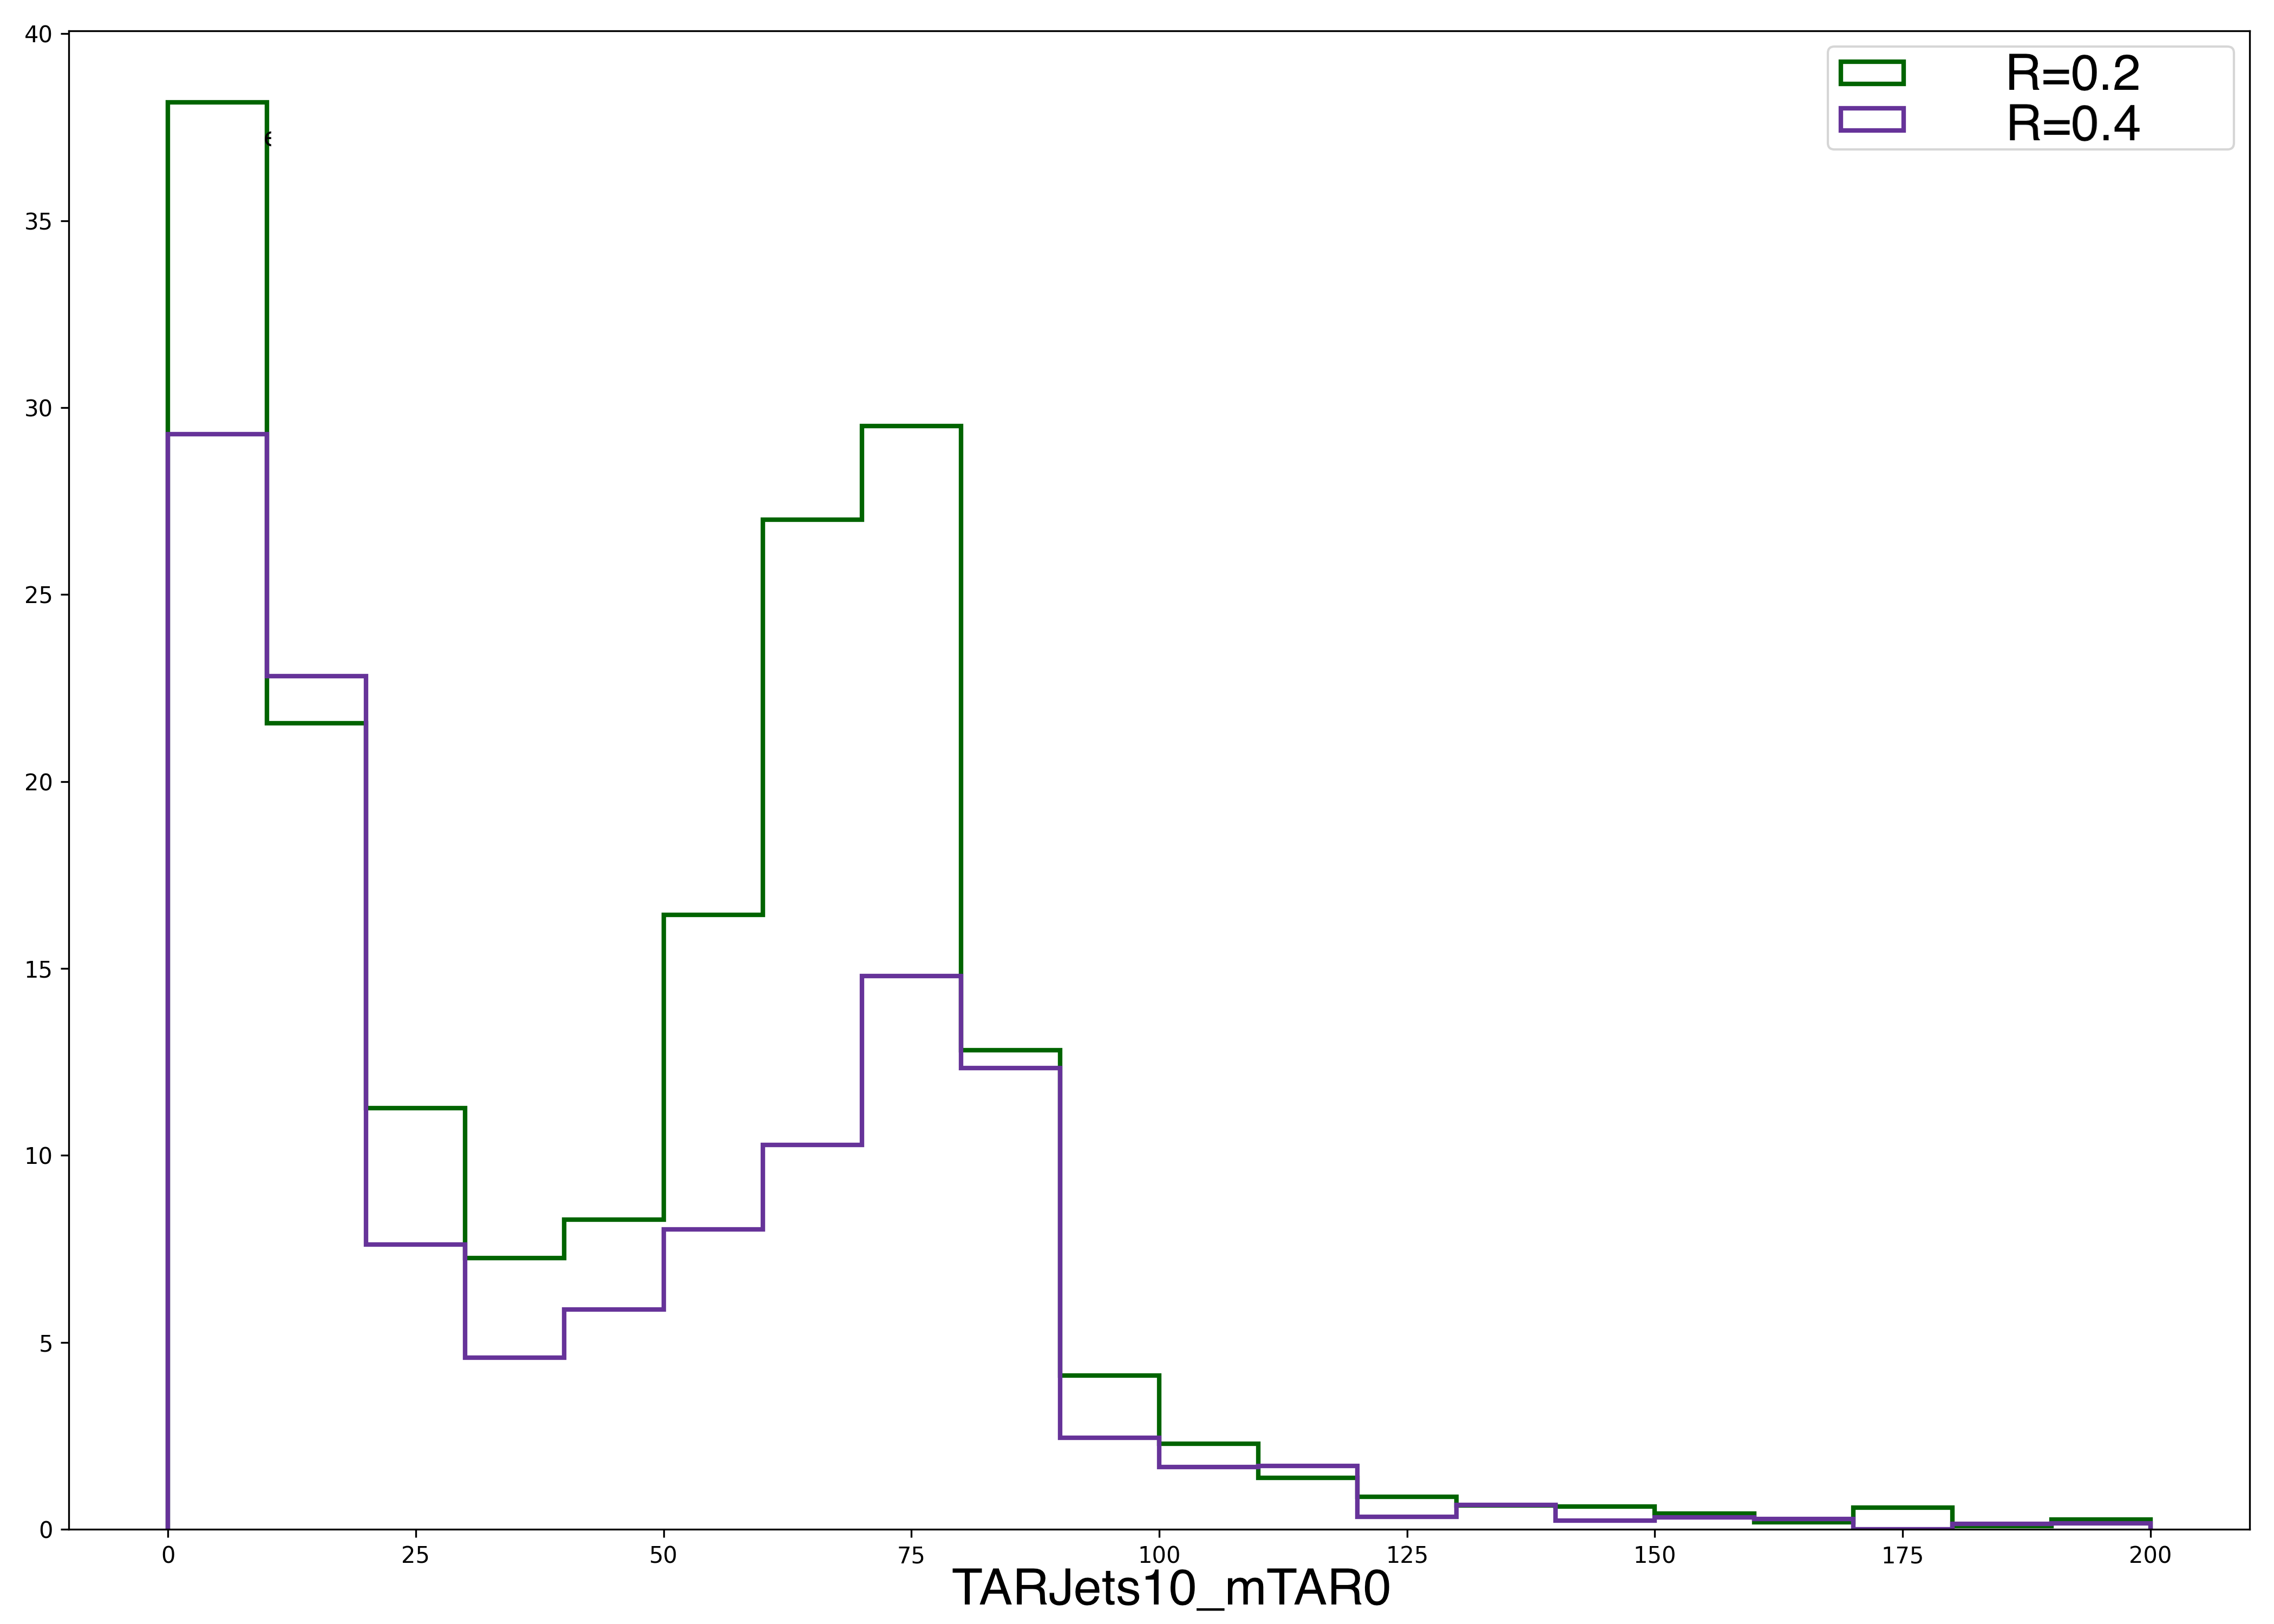
\includegraphics[width = 0.49\textwidth]{Figures/4/TAR/04_monoSww_semilep_zp1700_dm200_dh160.png}

     \caption{TAR jet mass distributions for two representative signal points compared with constituent \akt $R=0.4$ vs. \akt $R=0.2$ jets. Left: sample signal point at $(\ms, m_{Z^\prime})=(310, 500)~\GeV$. Right: sample signal point at $(\ms, m_{Z^\prime})=(160, 1700)~\GeV$}
     \label{fig:R04_TAR_plots}
\end{figure}


\subsection{Merged Signal Region Optimization}
\subsubsection{Asimov Significance}
The \merged signal is optimized in order to mazimize the expected Asimov discovery significance $Z$ given by:

\begin{equation}
  Z = \left[ 2(s+b)\left(
    \ln\left[ \frac{(s+b)(b+\sigma_b^2)}{b^2 + (s+b)\sigma_b^2} \right]
    - \frac{b^2}{\sigma_b^2}\ln\left[ 1 + \frac{\sigma_b^2 s}{b(b+\sigma_b^2)} \right]
  \right) \right]^\frac{1}{2}
  \label{eq:asimov}
\end{equation}

where $b$ is the expected total number of background events, $s$ is the expected total number of signal events, and $\sigma_b$ is the uncertainty on the expected total number of background events \cite{Asimov}. For a given set of selection criteria and signal mass point, this metric can be calculated from the MC simulated data by applying the criteria and counting the signal and background events and computing their uncertainties. It provides a metric to assess the expected sensitivity of the signal region to signal events.

\subsubsection{Optimization Approach}
In order to optimize the signal region selection a combination of an iterative visual approach and a computational approach were used. Visually, the distributions of analysis variables were studied to find areas of good discrimination, where a cut placement might improve sensitivity. A list of possible cuts in these areas of discrimination was then compiled to form a basis for the computational approach. In order to determine the oprimal combination of these possible cuts, a script was written to test all possible combinations (order of $10^6$) while computing the expected asimov significance of each. When calculating significance during optimization in addition to statistical uncertainty, a flat 20\% systematic uncertainty on the number of background events was applied to more realistically reflect the expected situation. Different signal points in the \ms-\mZp plane have different kinematic properties and therefore have different optimal selection. As a result, four signal points at the edge of the search sensitivity were selected for optimization:

\begin{itemize}
  \item (\ms, \mZp) = (310 GeV, 500 GeV),
  \item (\ms, \mZp) = (335 GeV, 1000 GeV),
  \item (\ms, \mZp) = (285 GeV, 1700 GeV),
  \item and (\ms, \mZp) = (210 GeV, 2100 GeV).
\end{itemize}

The cut combination with the higest mean expected Asimov significance over these four points was considered optimal. In early iterations of optimization, the number of signal events selected using the optimal selection criteria was undersireably low. As a result an additional requirement was implemented forcing the chosen criteria to maintain an expected yield of 15 expected signal events in the \merged signal region.

In order to minimize over-tuning the optimization on single events or statistical fluctuations the lattice of possible cuts were spaced widely enough to allow several MC events to fall between each placement. This does not, however, alleviate all concerns of a biased model. Some statistical fluctuation is still captured by optimization and un-checked this would lead to an under-prediction the standard model background because the selection is biased toward a low background content. To remove this bias, independent training and fitting data sets are used. All optimization was performed using the set of MC samples produced using Sherpa 2.2.1. The samples produced with Sherpa 2.2.10 provide a statistically independent and more statistically rich data set which is used for validation and fitting. This means that the MC data used for fitting is isolated from the optimization of selection criteria.

Large negative weight removal.

\subsubsection{Optimization Variables}
Many analysis variables were explored for potential sensitivity, and those selected as having the best discrimination potential were tested in the final optimization. Presented below is a list of variables tested and their meaning.

\begin{itemize}
  \item \textbf{\met} and \metsig: Missing transverse momentum and its significance.
  \item \textbf{$p_T(\ell)$}: Transverse momentum of signal lepton.
  \item \textbf{\mtlepmet}: Transverse mass of lepton and \met system, given by
  \begin{equation}
  \mtlepmet = \sqrt{2 p_{\text{T},\ell} \met \left( 1 - \cos(\phi_\ell - \phi_{\met}) \right) }
  \end{equation}
  \item \textbf{\mTAR}: Mass of the \pT-leading TAR jet calculated from the rescaled matched tracks.
  \item \textbf{\ptTAR}: Trasverse momentum of the leading TAR jet.
  \item \textbf{\DtwoTAR}: Energy correlation function of the TAR jet, which helps to identify two-pronged jet substructure \cite{DTwo}.
  \item \textbf{TAR Jet $\tau_{42}^{WTA}$ and $\tau_{21}^{WTA}$}: N-Subjettiness ratios of the leading TAR jet, to identify two-pronged substructure \cite{Tau42}.
\end{itemize}

In addition, a two-dimensional cut in the \met-$p_T(\ell)$ plane was considered during optimization.

\subsubsection{Optimized Selection}


The maximum mean expected significance across the four selected signal points was found to be achieved using the selection shown in Table \ref{tab:mergedselection_reopt}.

\begin{table}[htbp]
  \centering
  \begin{tabular}{c|c|c}
    \toprule
    \textbf{variable}  &  \textbf{requirement} &  \textbf{reason}  \\
    \midrule
    \NTAR  &  $>0$ & \Wcand reconstruction \\
    \mtlepmet  &  $>220\,\GeV$ & W+Jets Background Reduction\\
    \mTAR &  $[68,89]\,\GeV$ & \Wcand reconstruction \\
    \metsig  &  $>16$ & Select for high \met \\
    \dRTARl &  $<1.2$ & Select for boosted \Wcand+$\ell\nu$ system \\
    \DtwoTAR  &  $<1.1$ & 2 Pronged W->qq Reco \\
    \bottomrule
  \end{tabular}
  \caption{Optimized selection criteria for the \merged category signal region.}
  \label{tab:mergedselection_reopt}
\end{table}

In order to validate the choice of selection criteria ``N-1" plots were produced which show the distribution of a variable with all but the cut on that variable applied. The expected asimov significance of placing a cut at each bin edge is then also calculated. These plots were produced using the W+Jets and Z+Jets samples produced in Sherpa 2.2.10 and are shown in Figure ~. They therefore demonstrates whether cuts are still placed at optimal or near-optimal locations using the final samples.

The plots validate the choice of cut placements, which are still at or near maximal significance.

\begin{figure}[htbp]
  \centering

     \begin{subfigure}{0.49\textwidth}
     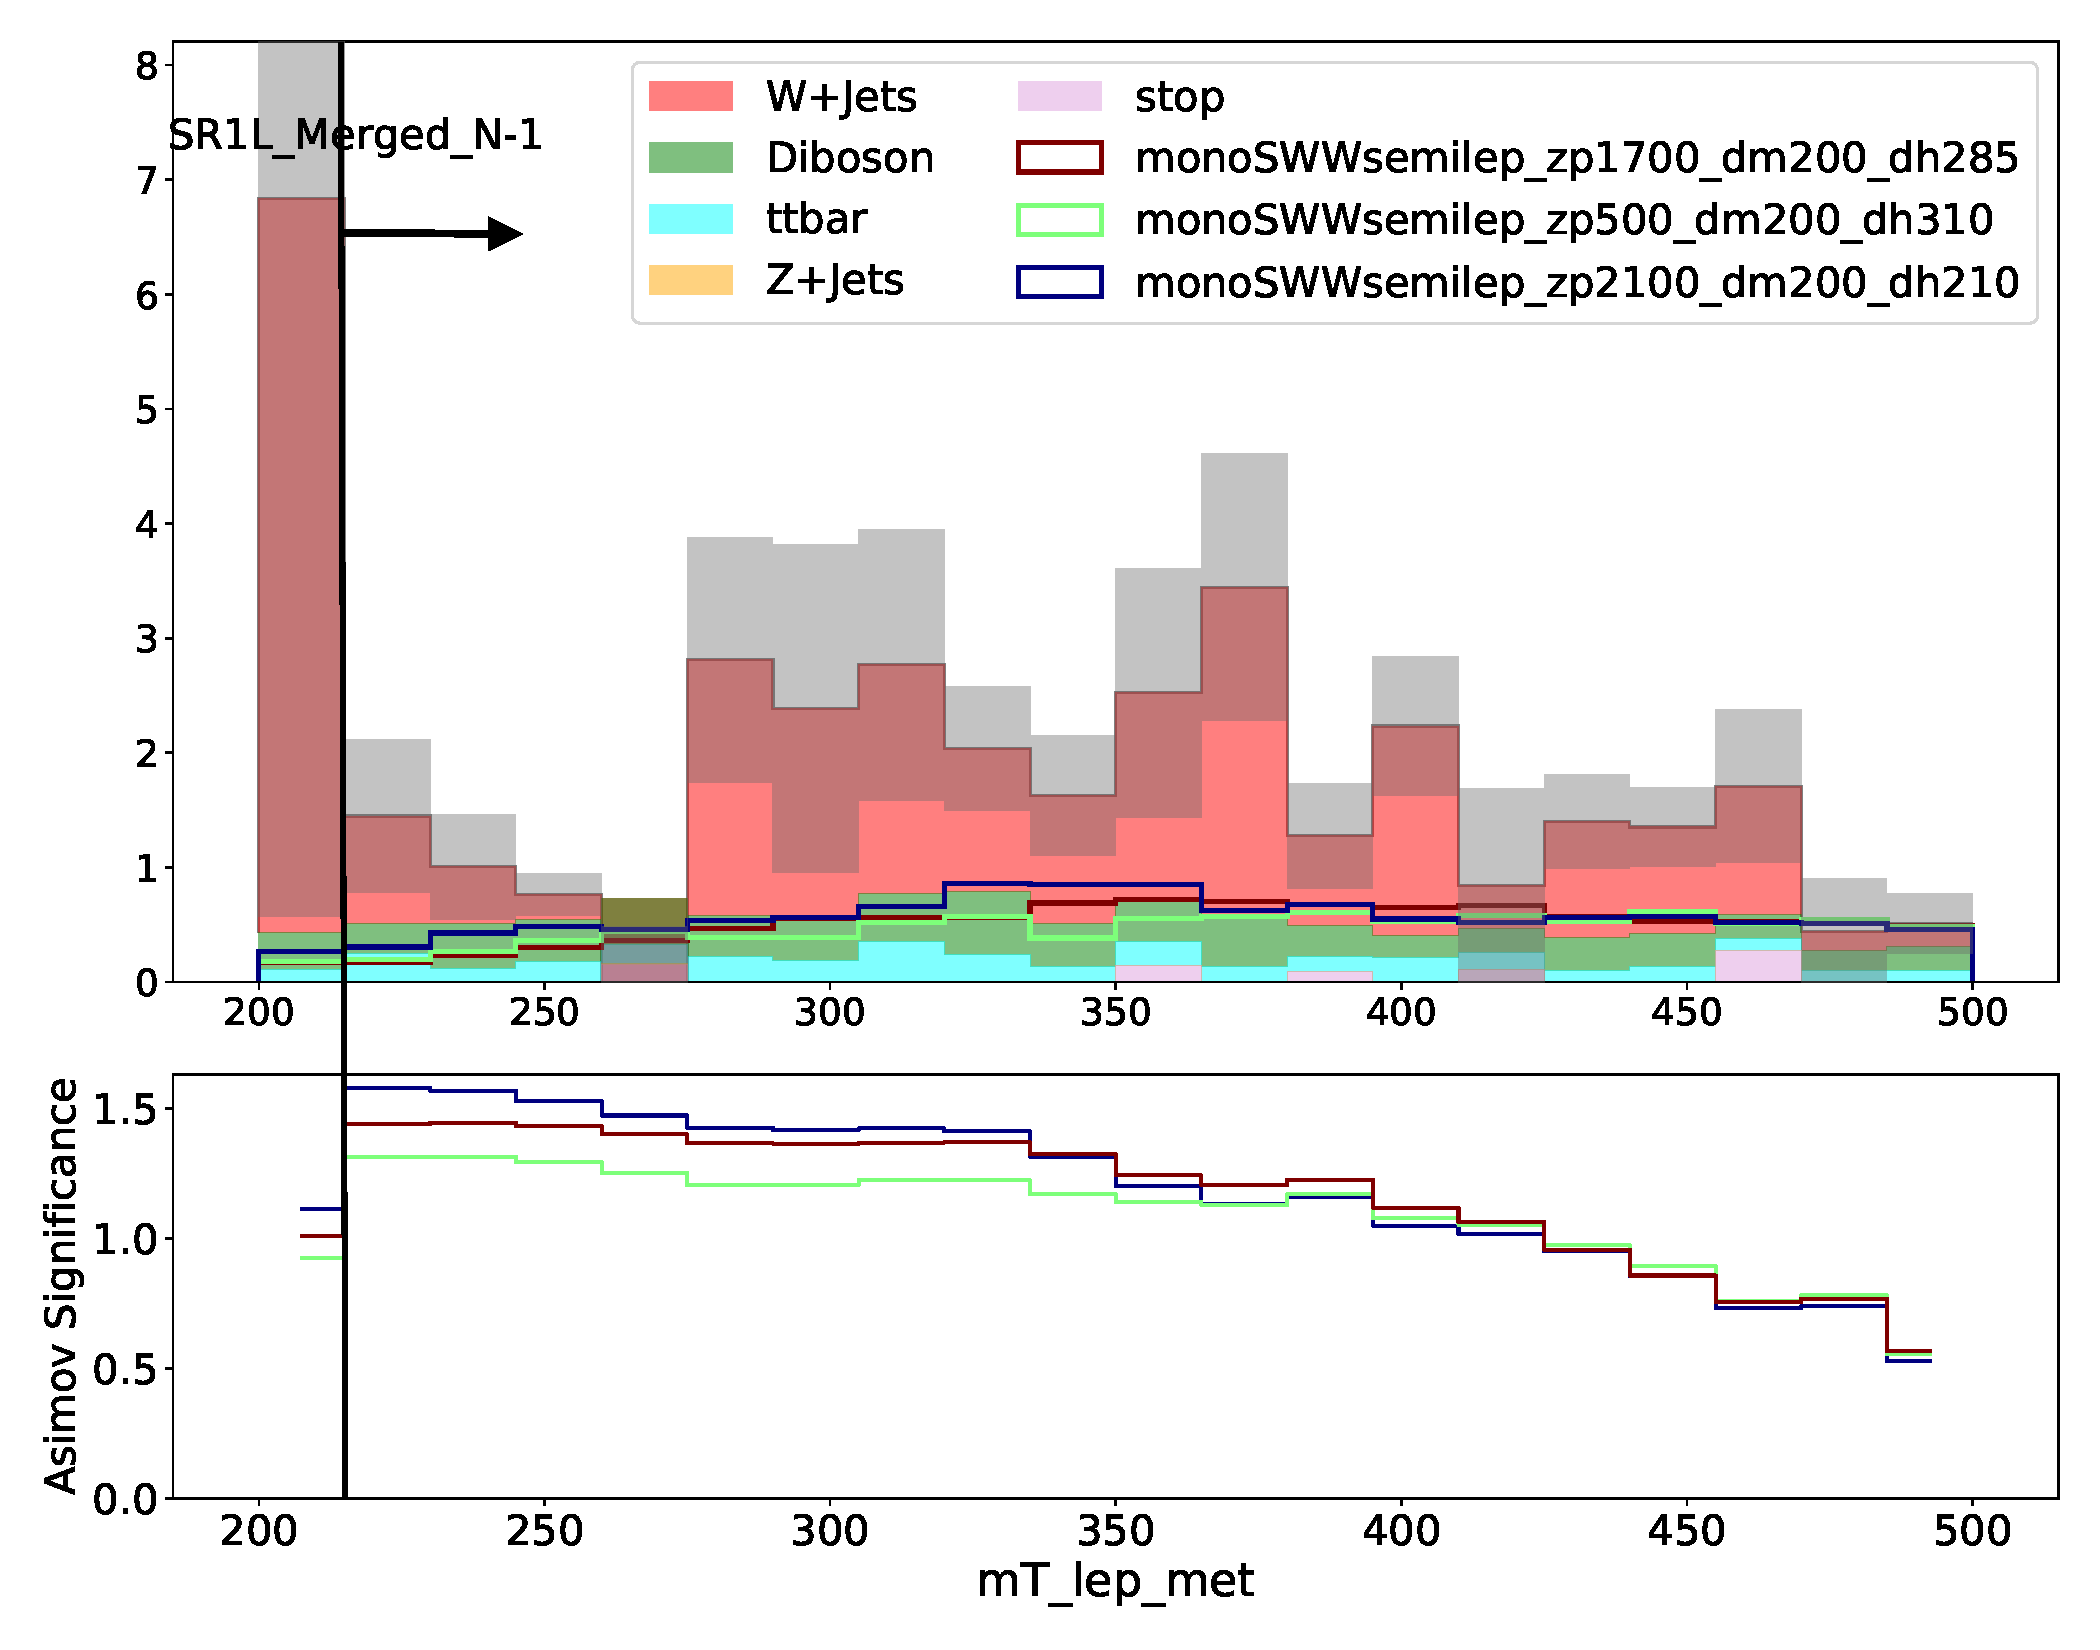
\includegraphics[width = 0.98\textwidth]{Figures/4/N1m/mT_lep_met.pdf}
     \caption{\mtlepmet}
     \end{subfigure}
     \begin{subfigure}{0.49\textwidth}
     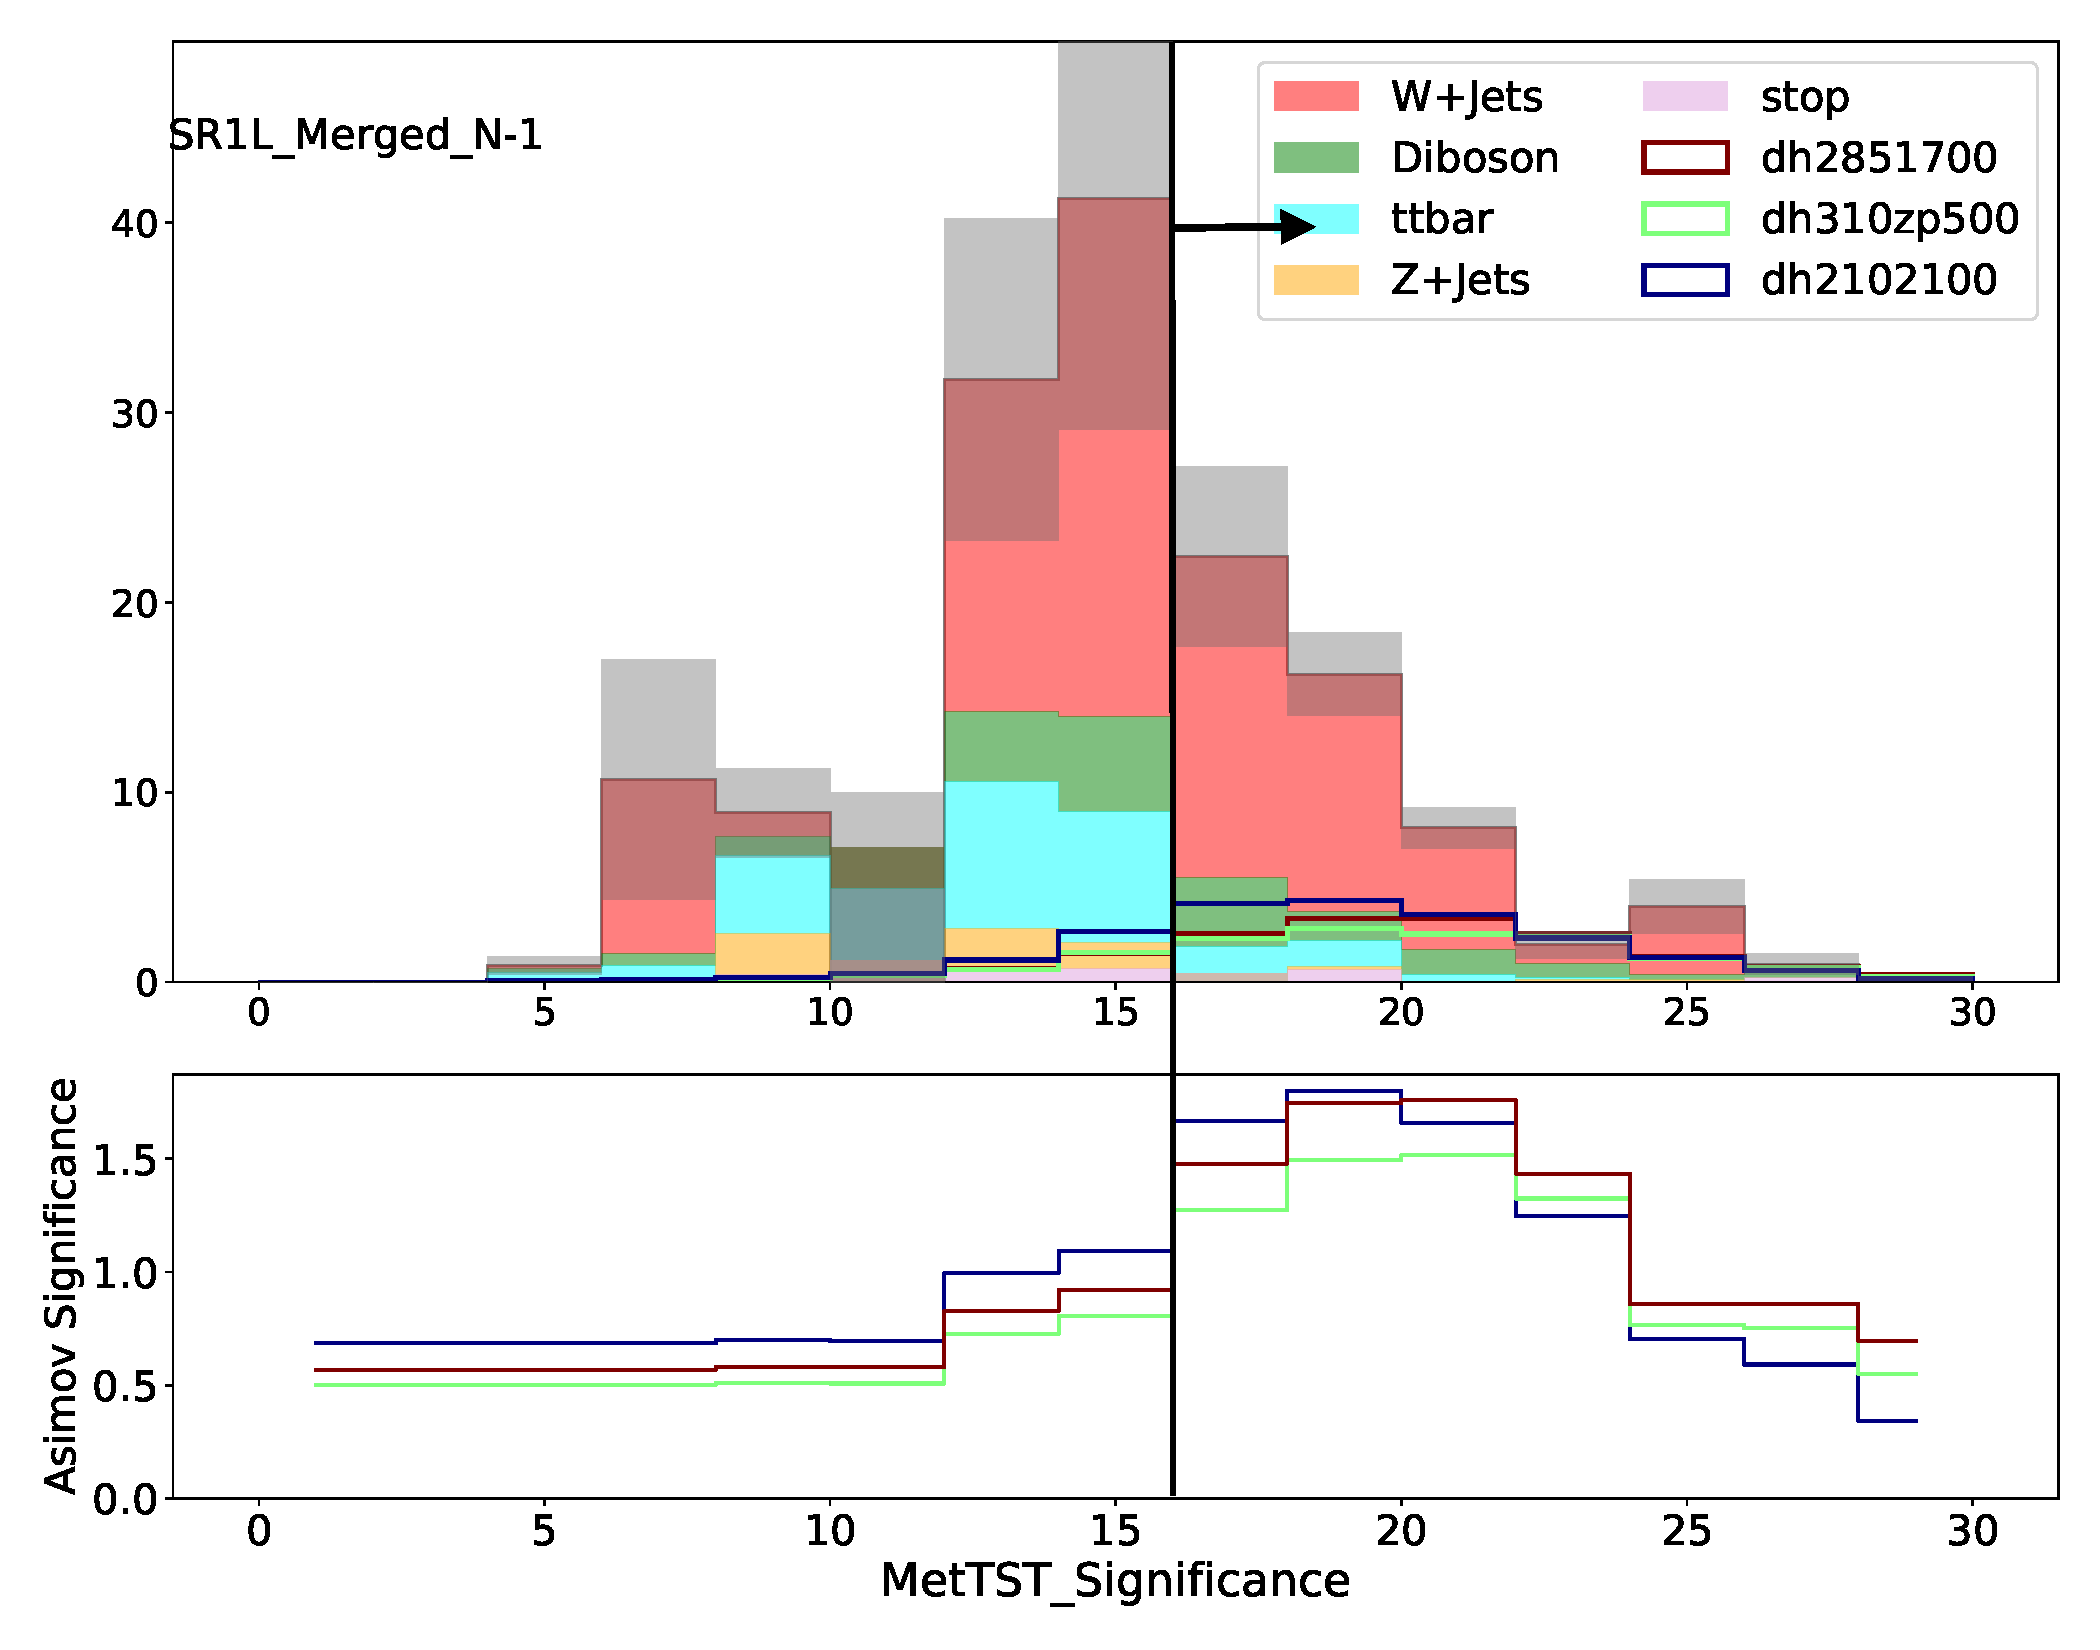
\includegraphics[width = 0.98\textwidth]{Figures/4/N1m/MetTST_Significance.pdf}
     \caption{\metsig}
     \end{subfigure}
     \begin{subfigure}{0.49\textwidth}
     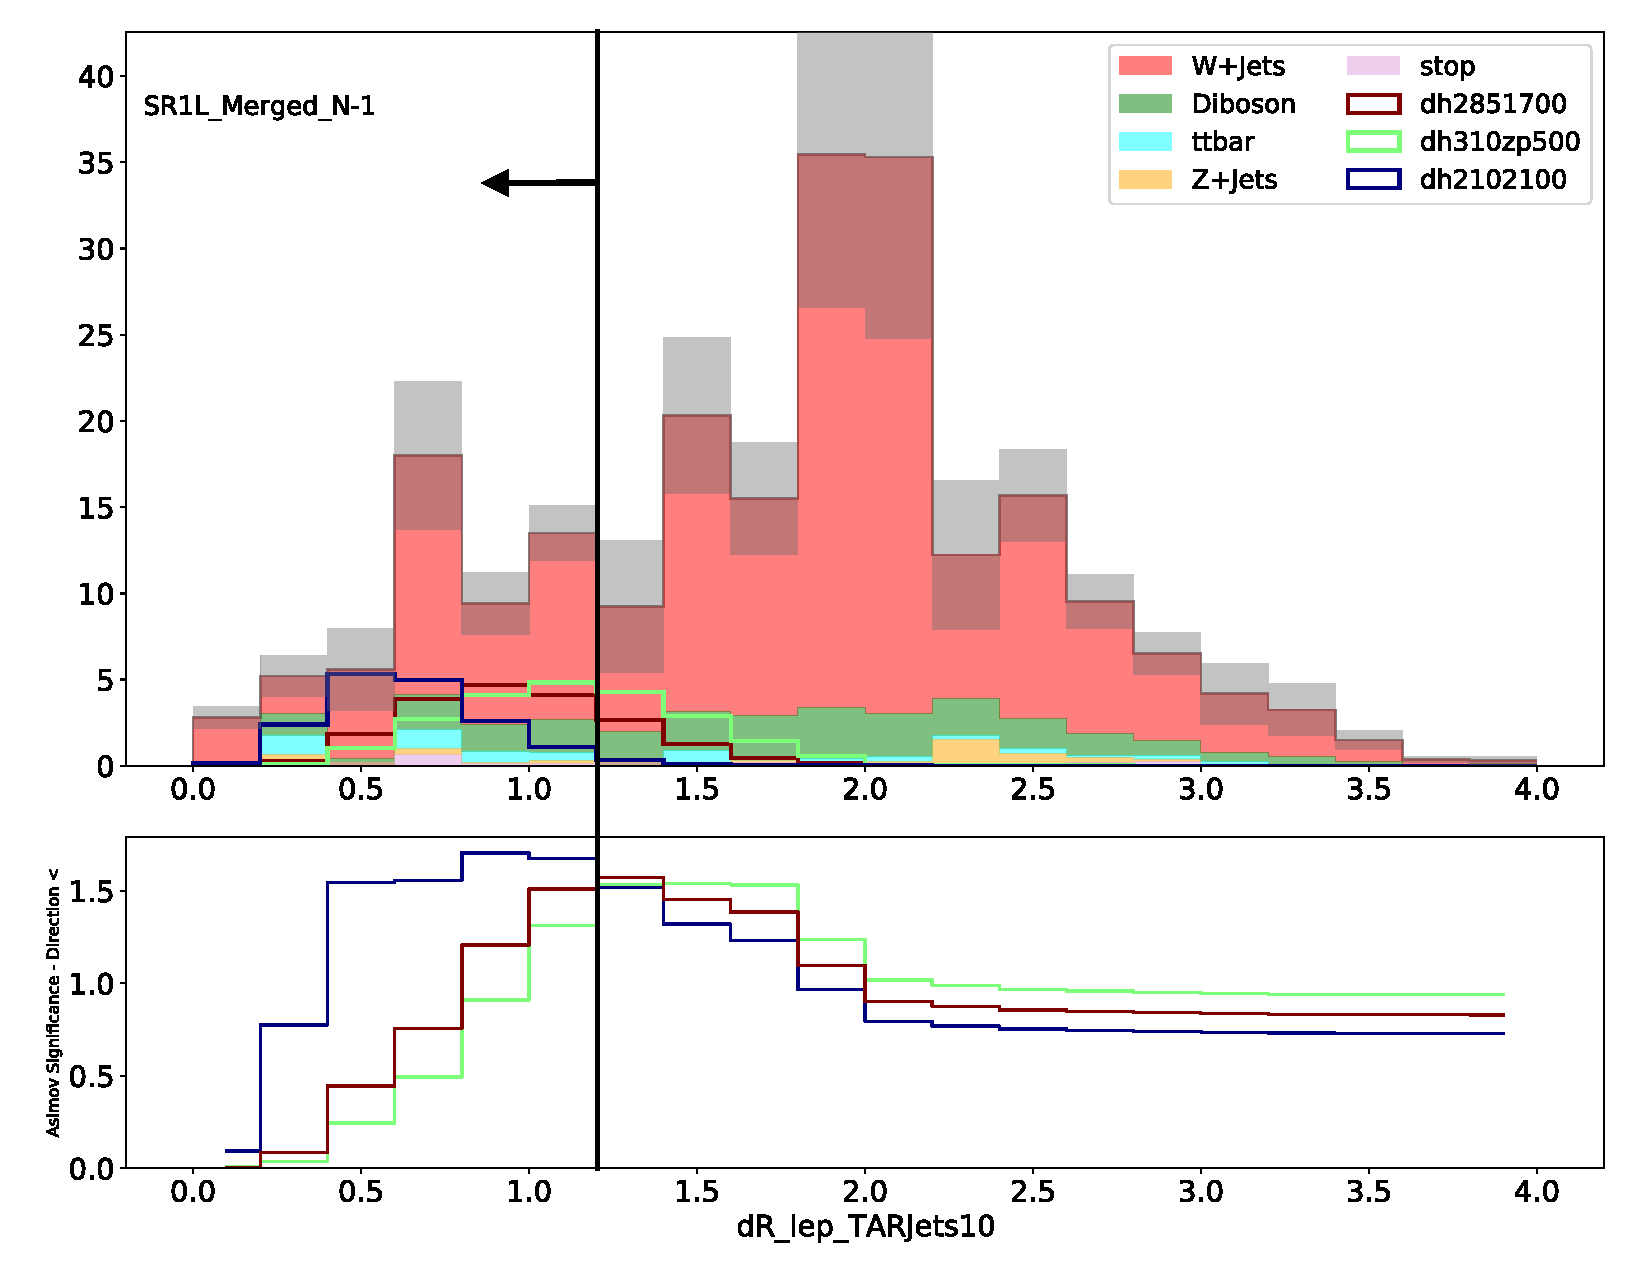
\includegraphics[width = 0.98\textwidth]{Figures/4/N1m/dR_lep_TARJets10.pdf}
     \caption{\drTARl}
     \end{subfigure}
     \begin{subfigure}{0.49\textwidth}
     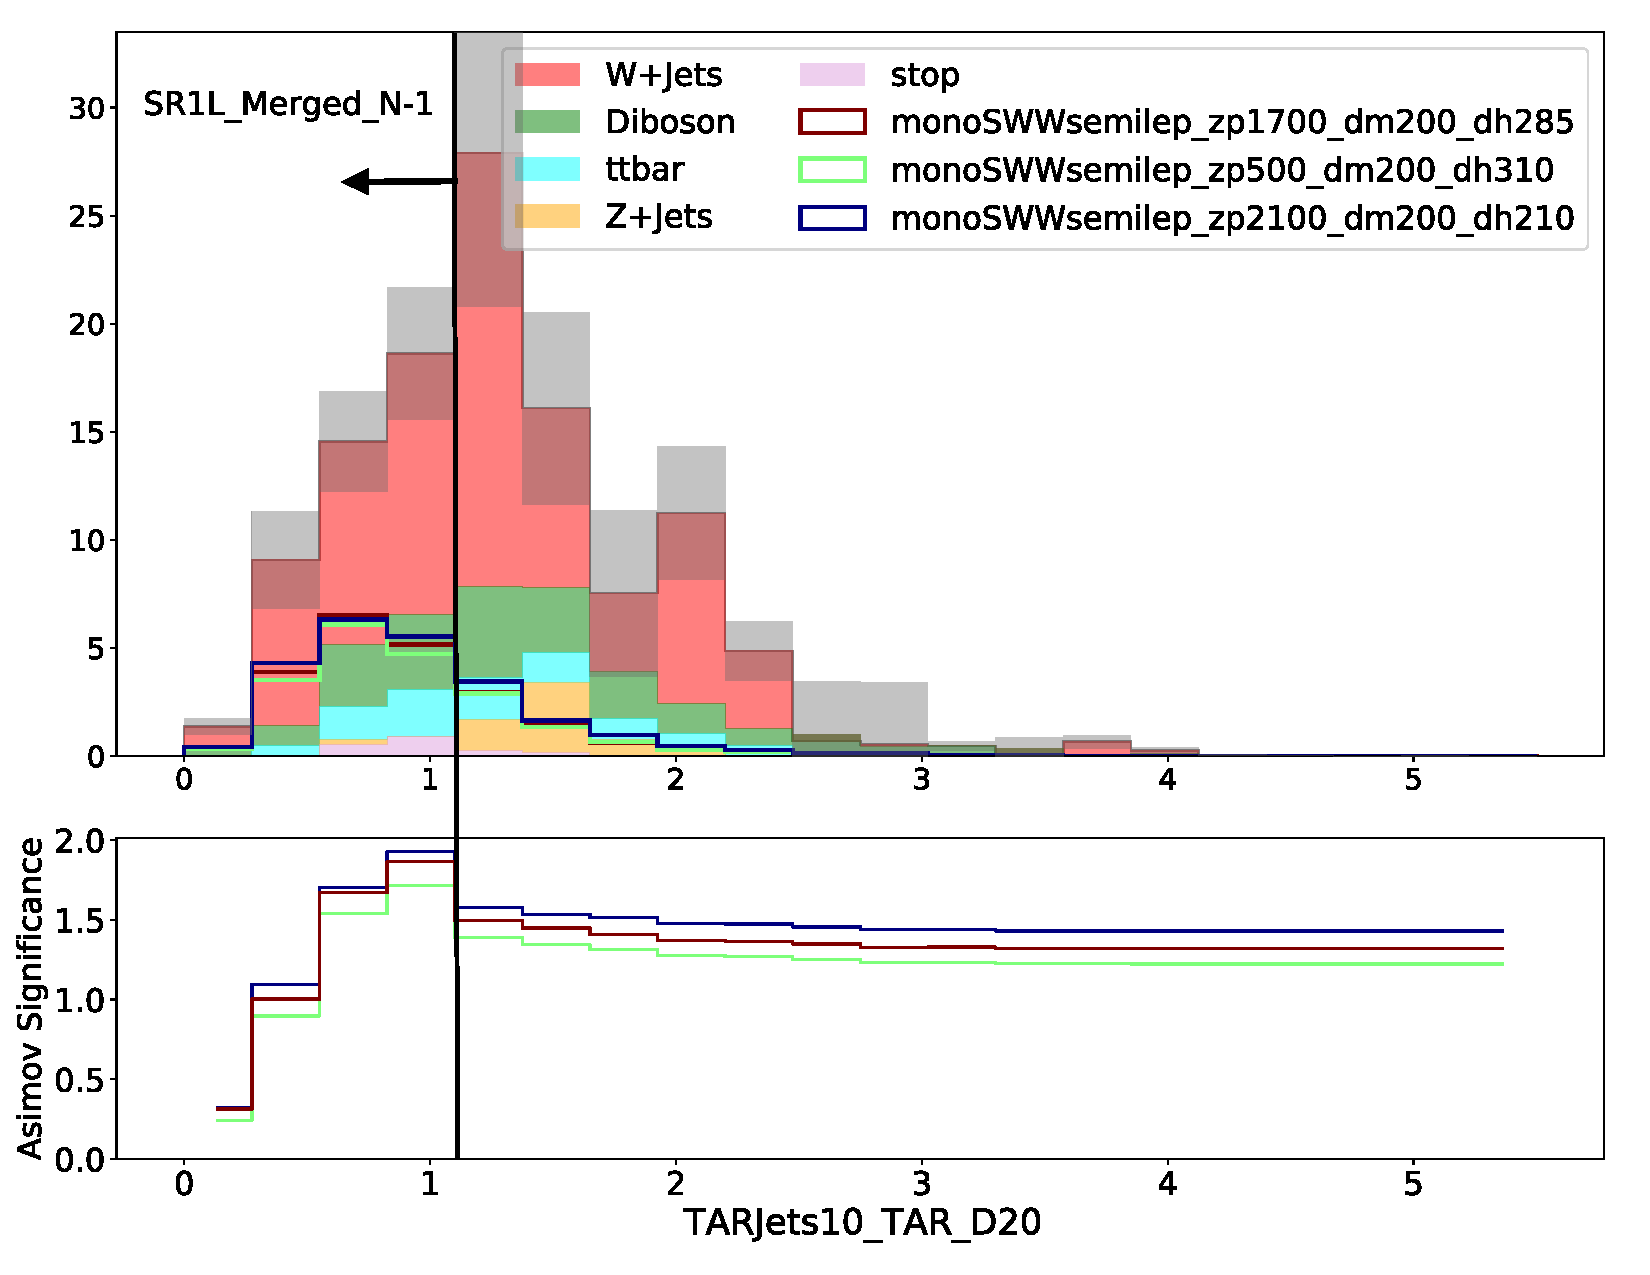
\includegraphics[width = 0.98\textwidth]{Figures/4/N1m/TARJets10_TAR_D20.pdf}
     \caption{\DtwoTAR}
     \end{subfigure}
     \begin{subfigure}{0.49\textwidth}
     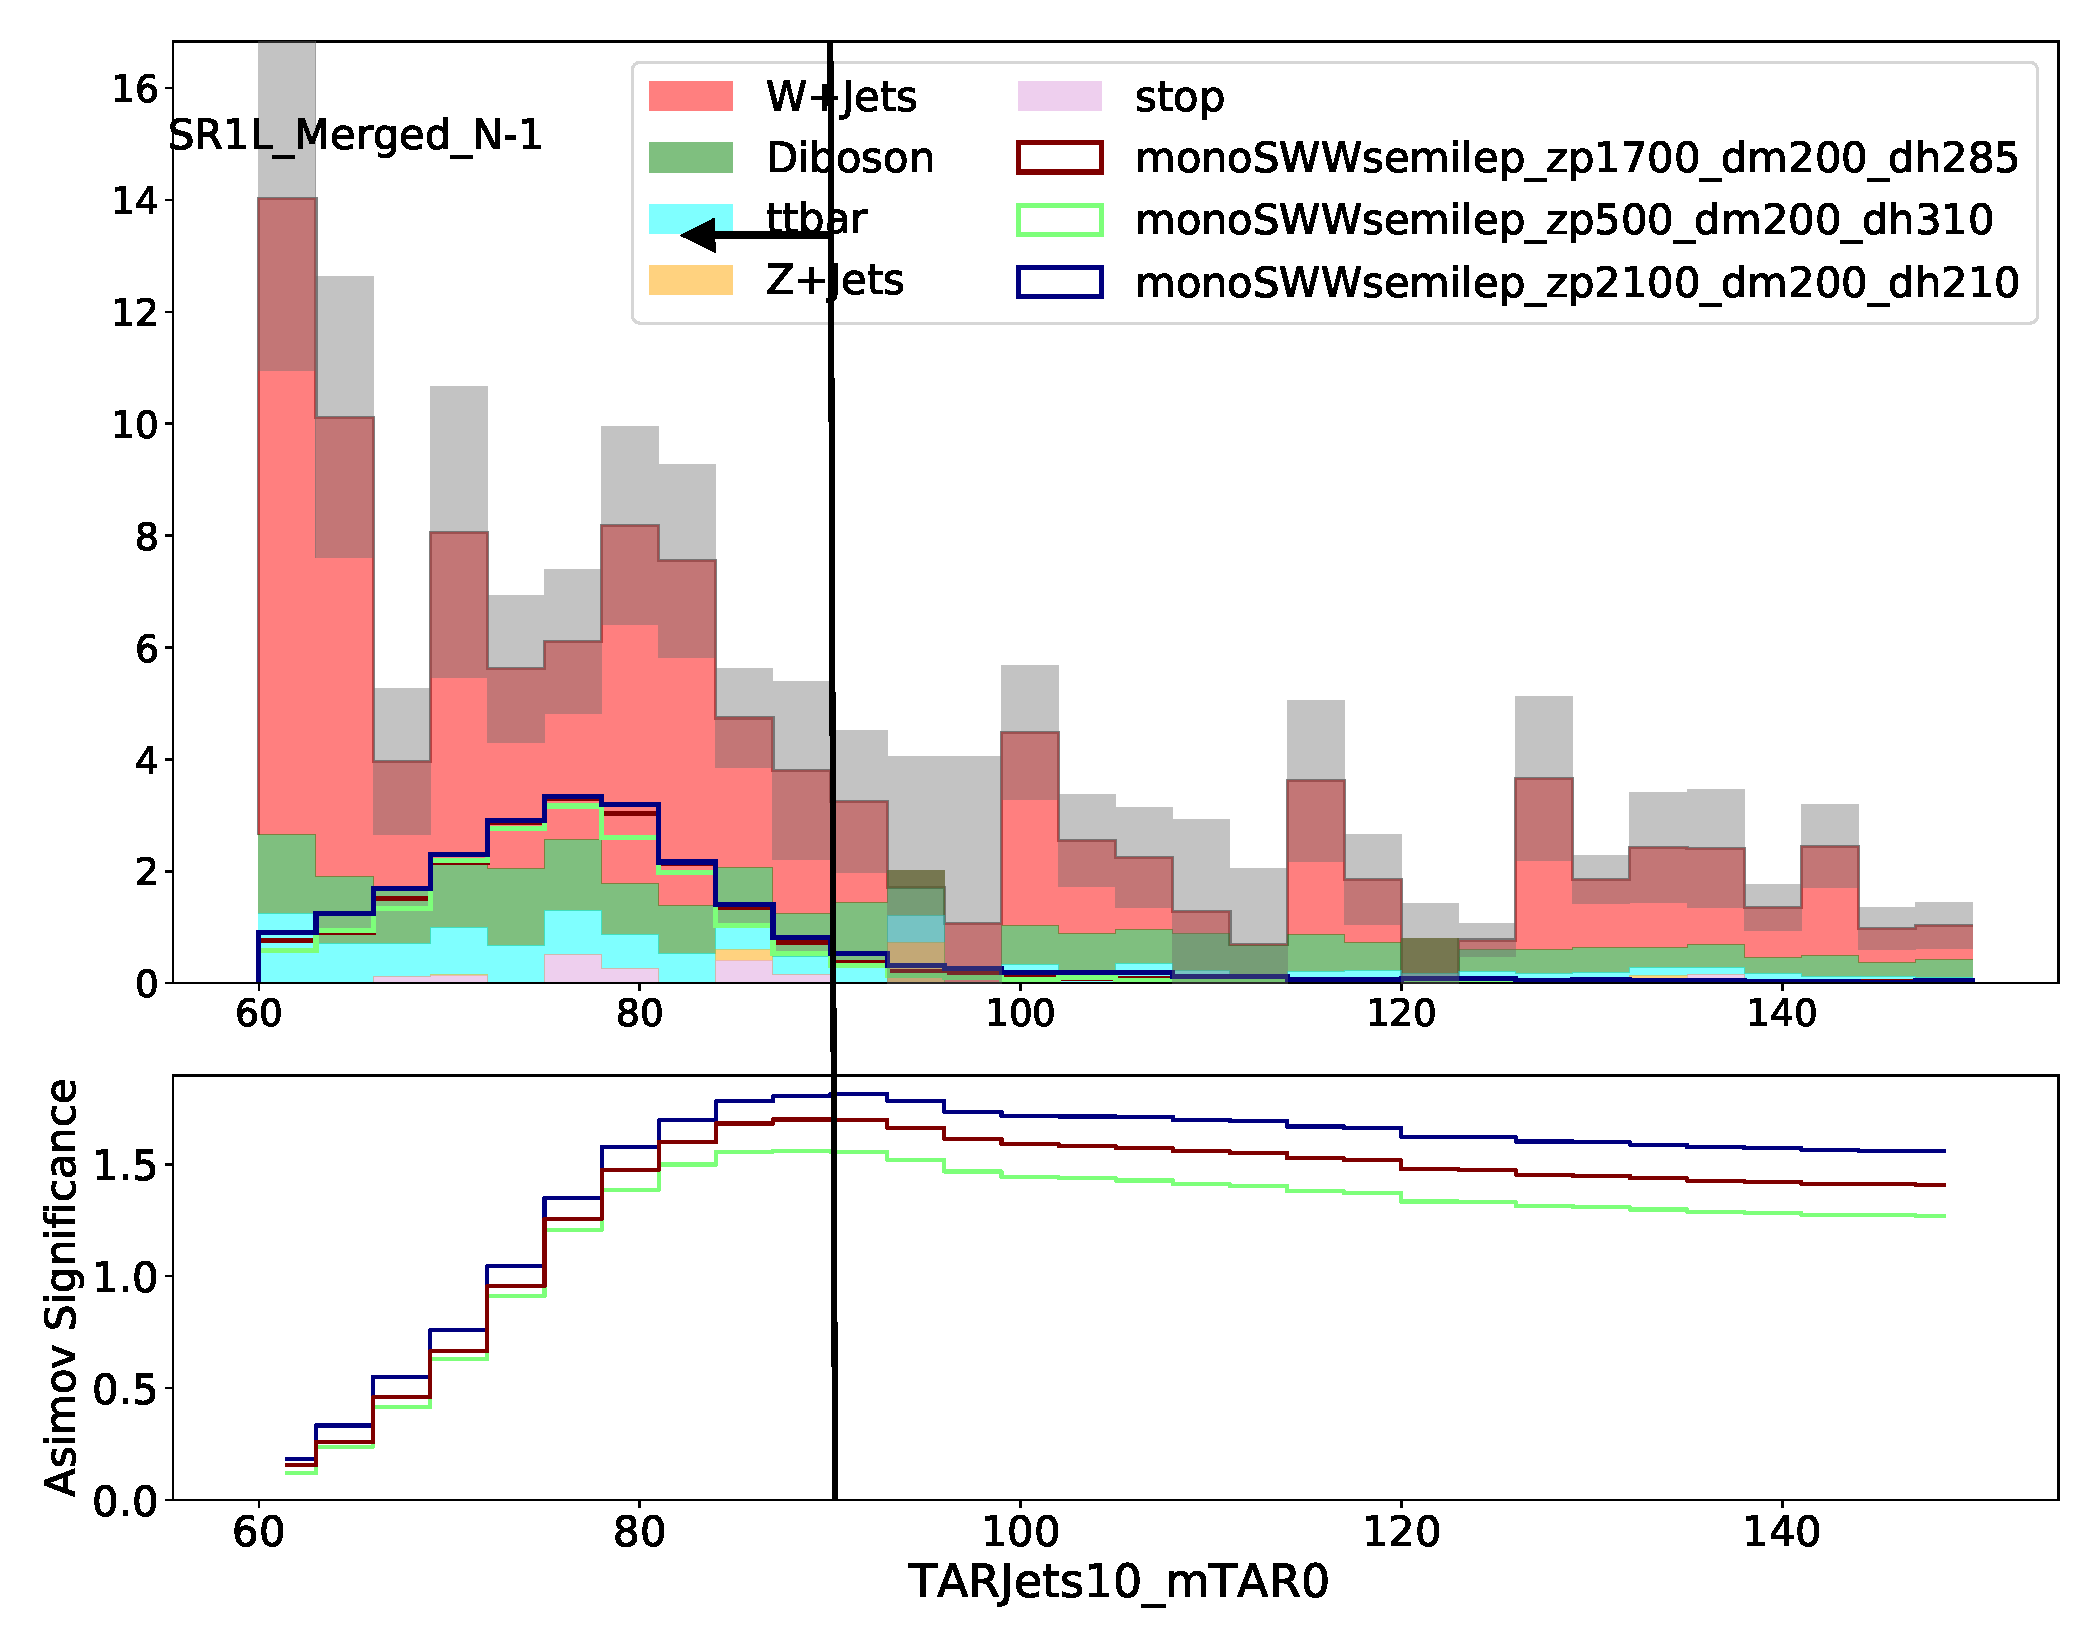
\includegraphics[width = 0.98\textwidth]{Figures/4/N1m/TARJets10_mTAR0.pdf}
     \caption{\mTAR}
     \end{subfigure}
     \begin{subfigure}{0.49\textwidth}
     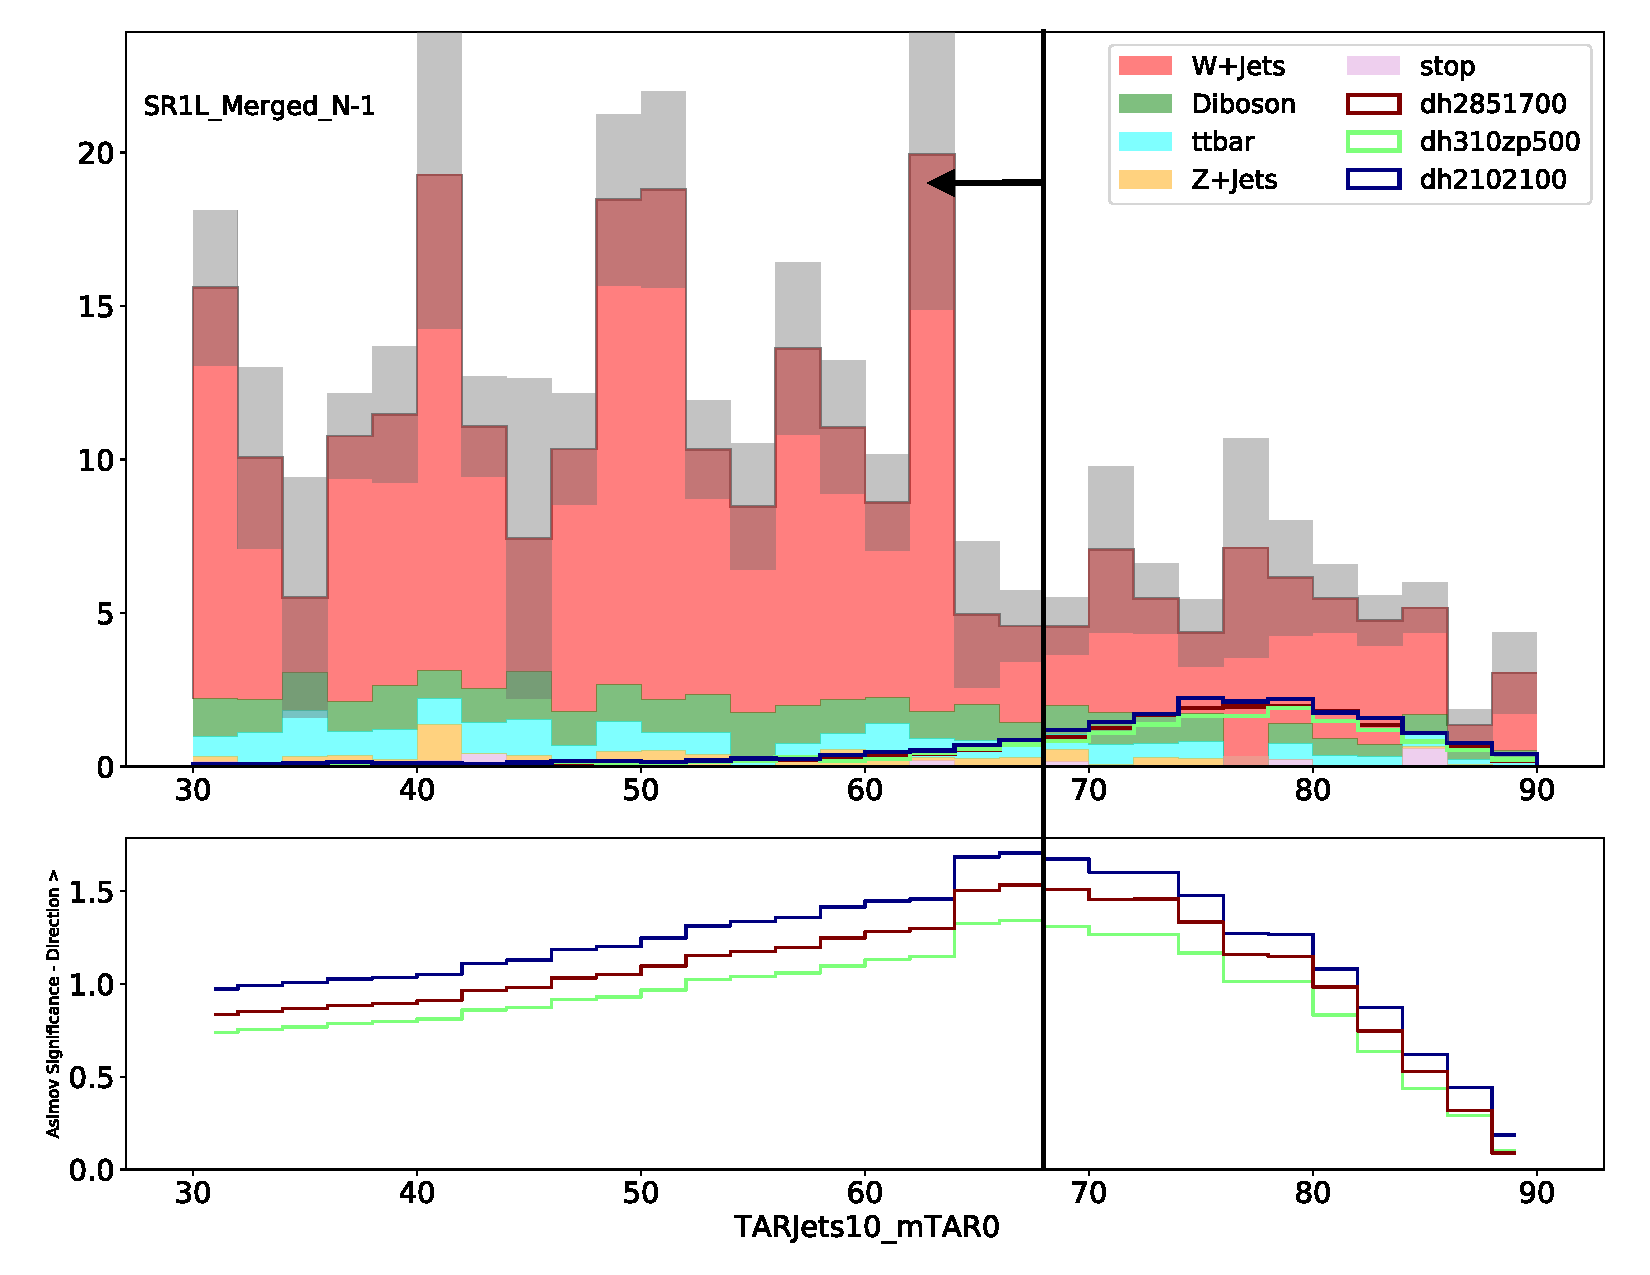
\includegraphics[width = 0.98\textwidth]{Figures/4/N1m/TARJets10_mTAR02.pdf}
     \caption{\mTAR}
     \end{subfigure}

     \caption{N-1 plots in the \merged signal region.}
     \label{fig:SRN1}
  \end{figure}

\section{Resolved Signal Region}
Due to the highly boosted nature of most signal events, the hadronic W-decay products are most often able to be resconstructed as a TAR jet. As a result, the \resolved signal region is considerably less sensitive than the \merged signal region, but does provide an important enhancement especially at low $s$ mass where the least boost is experienced. The \resolved signal region selection criteria are listed in Table ~.

\section{\ttbar Control Regions}
A control region is used to help constrain one or more sources of background in an analysis. It is designed as a region that covers a similar but orthogonal area of phasse space to the signal region and is expected to contain many fewer signal events. As a result, the number of ATLAS data and MC simulated SM data events should in theory match very closely. Thus, a comparison ATLAS and MC data can be used in this region to help constrain the SM background predictions of MC in the signal region, ideally increasing accuracy and reducing uncertainty. \ttbar is one of the three leading backgrounds in the both signal regions and this, along with a relatively simple path to a control region definition motivates creating one for each signal region.

Due to the fact that top quarks decay primarily to an W boson and $b$-quark, the principal cut excluding \ttbar events from the signal regions is the veto of any events containing a b-tagged \akt $R=0.4$ jet. A natural path to defining a similar but orthogonal region rich in \ttbar events would therefore be to simply reverse this cut and require at least 1 b-tagged jet. This scenario was found to be too signal rich, however, with only a reduction by factor of 10 and 4 in mean MC $\frac{signal}{background}$ from the \merged and \resolved signal regions.

To ameliorate this, the b-jet requirement was further pushed to 2 or more b-jets in the control region. This change sufficiently reduced signal contamination, but in the \merged control region it had the additional consequence of substantially reducing the number of events in the region, thereby reducing its statistical power.  In response the \metsig cut was also loosened in the \merged \ttbar control region to \metsig > 12. Figure \ref{fig:ttbar_metsig_placement}, which shows the number of weighted \ttbar events expected in the \merged control region for a given \metsig cut was used to motivate this choice.

\begin{figure}[htbp]
    \centering
       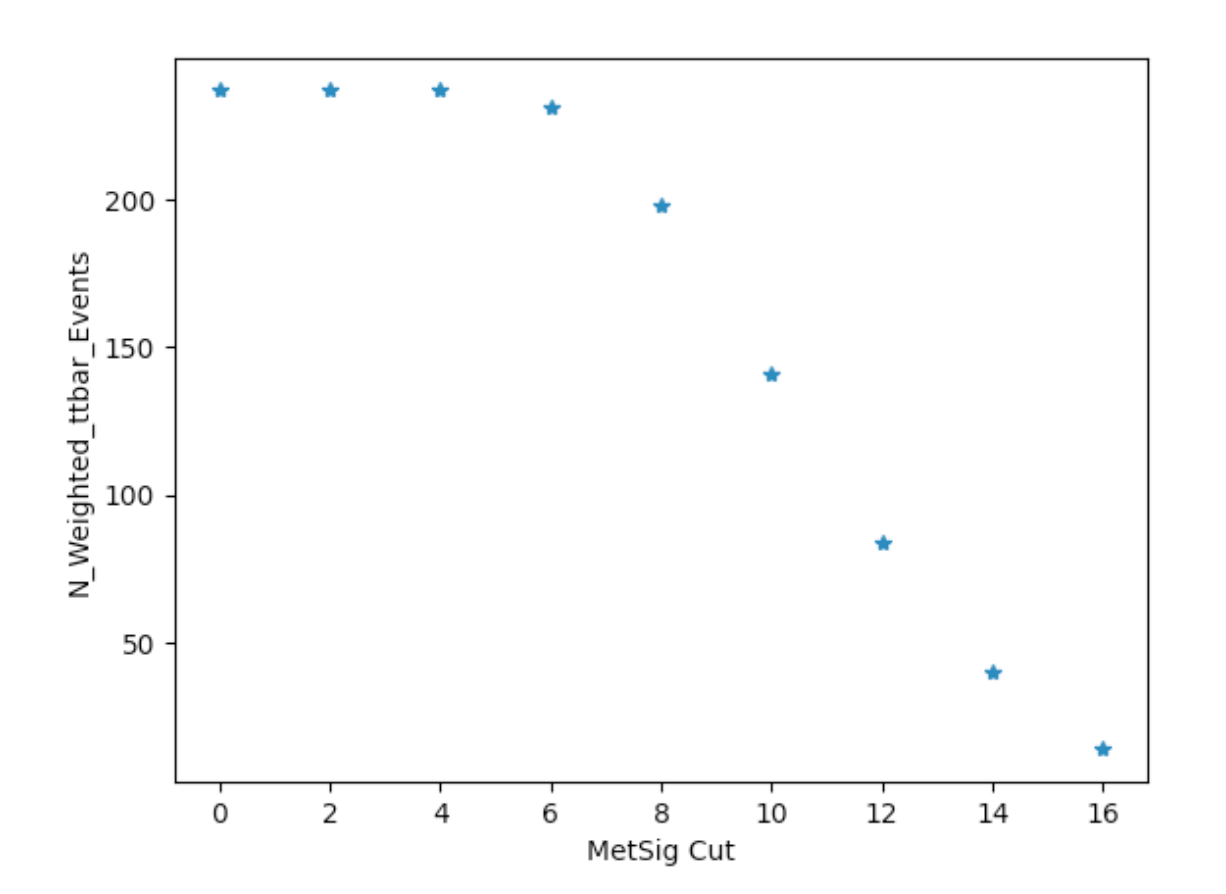
\includegraphics[width = 0.80\textwidth]{Figures/4/ttbarCR/ttbar_metsig_placement.png}
       \caption{\ttbar yield in the \merged \ttbar control region for various \met significance cut placements}
       \label{fig:ttbar_metsig_placement}
\end{figure}

Table ~ summarizes the differences in selection criteria between the \merged and \resolved signal and \ttbar control regions.

Figures ~ and ~ show comparisons of the distributions of MC and ATLAS data in the \ttbar control regions. These demonstrate a slight over-prediction of yield from MC in the \merged region, which will be used to constrain the \ttbar background in the signal region. The difference between data and MC distributions does not show a strong correlation with any of the analysis variables.

\begin{figure}[htbp]
  \centering

     \begin{subfigure}{0.49\textwidth}
     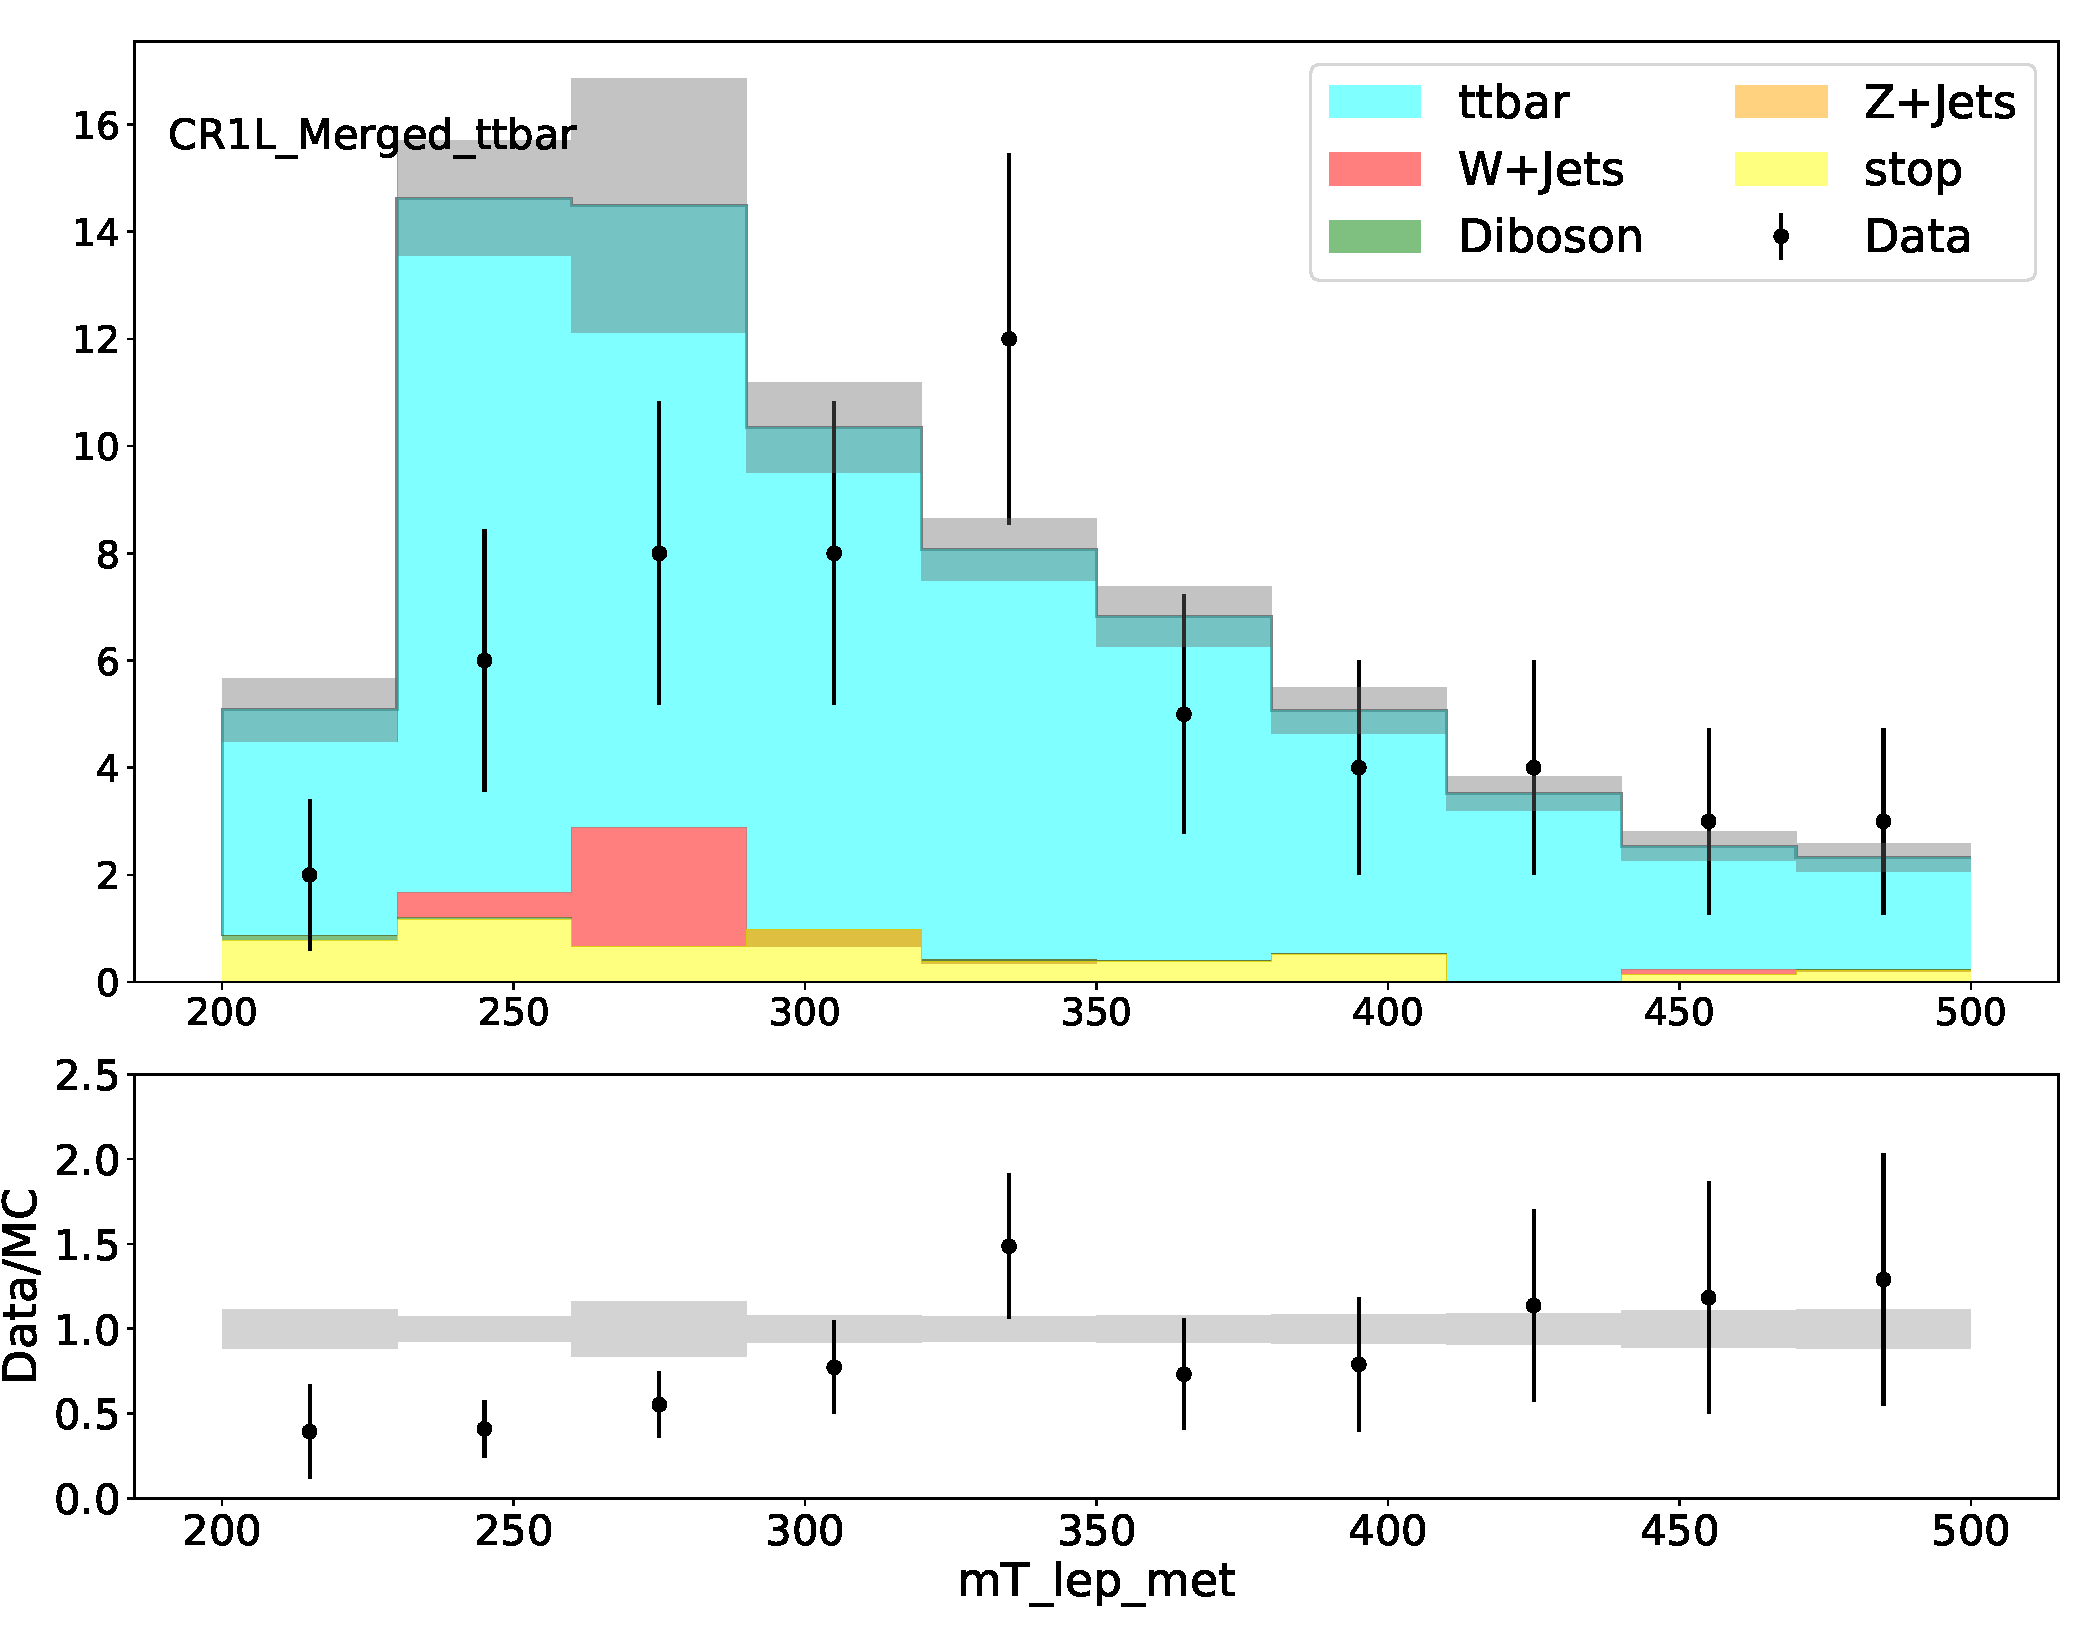
\includegraphics[width = 0.98\textwidth]{Figures/4/datamc/CR1L_Merged_ttbar/mT_lep_met.pdf}
     \caption{\mtlepmet}
     \end{subfigure}
     \begin{subfigure}{0.49\textwidth}
     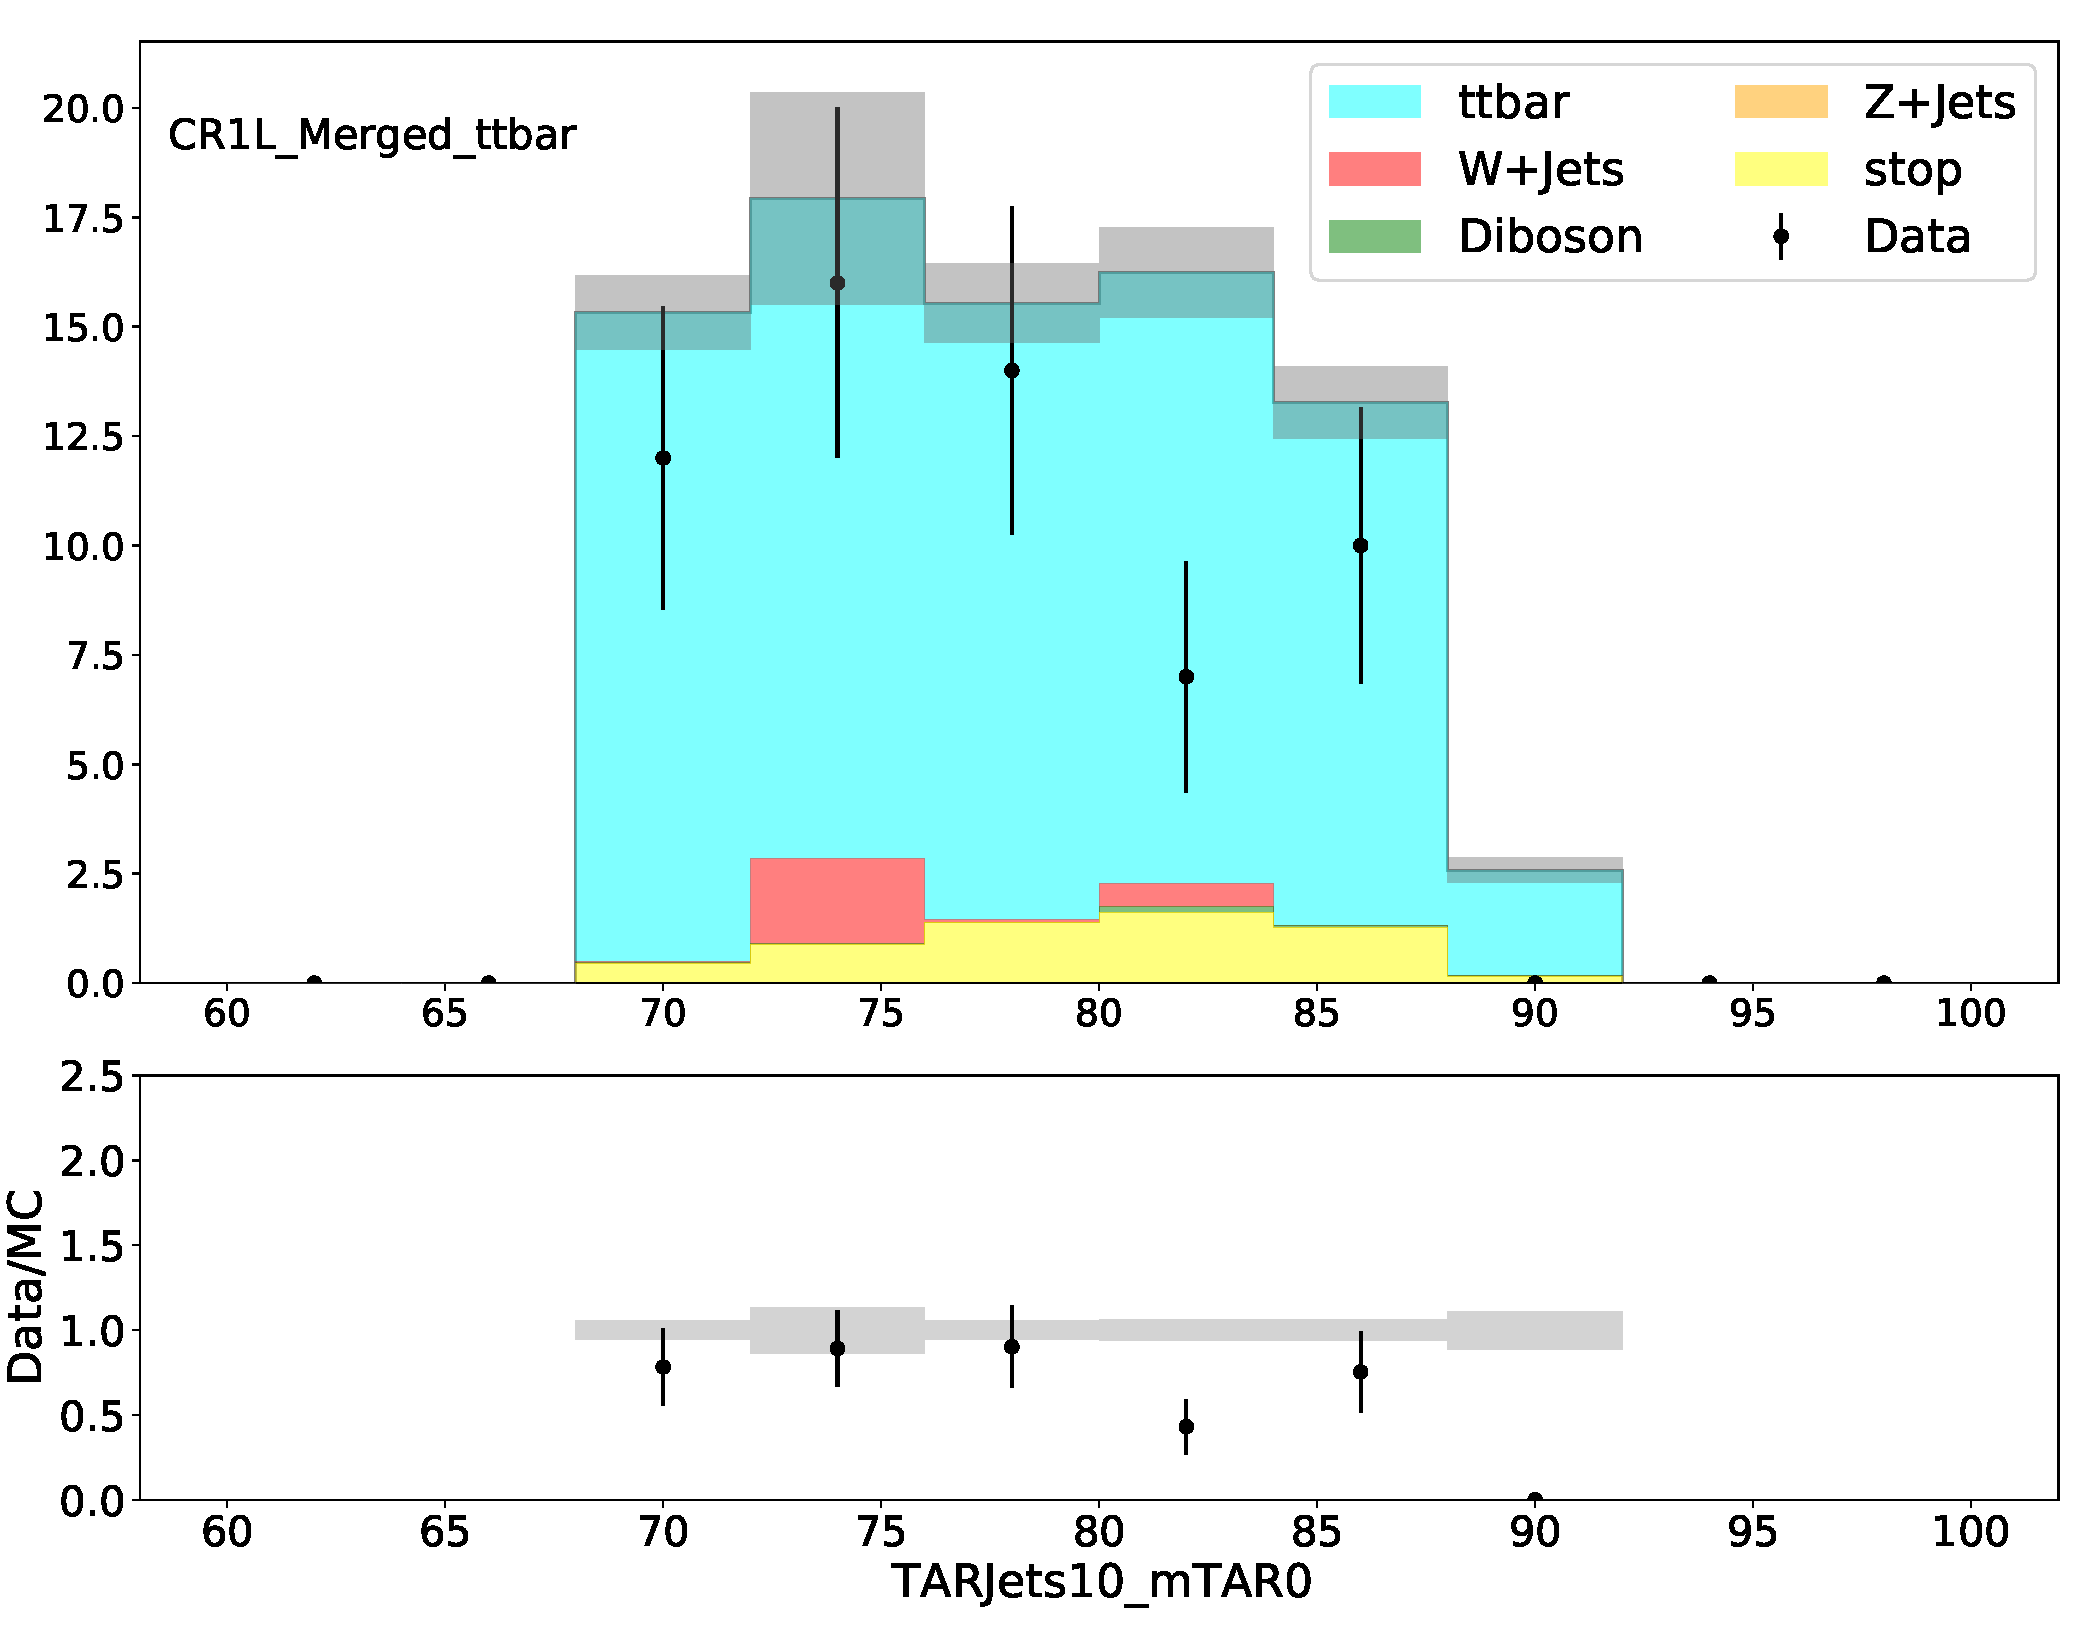
\includegraphics[width = 0.98\textwidth]{Figures/4/datamc/CR1L_Merged_ttbar/TARJets10_mTAR0.pdf}
     \caption{\mTAR}
     \end{subfigure}
     \begin{subfigure}{0.49\textwidth}
     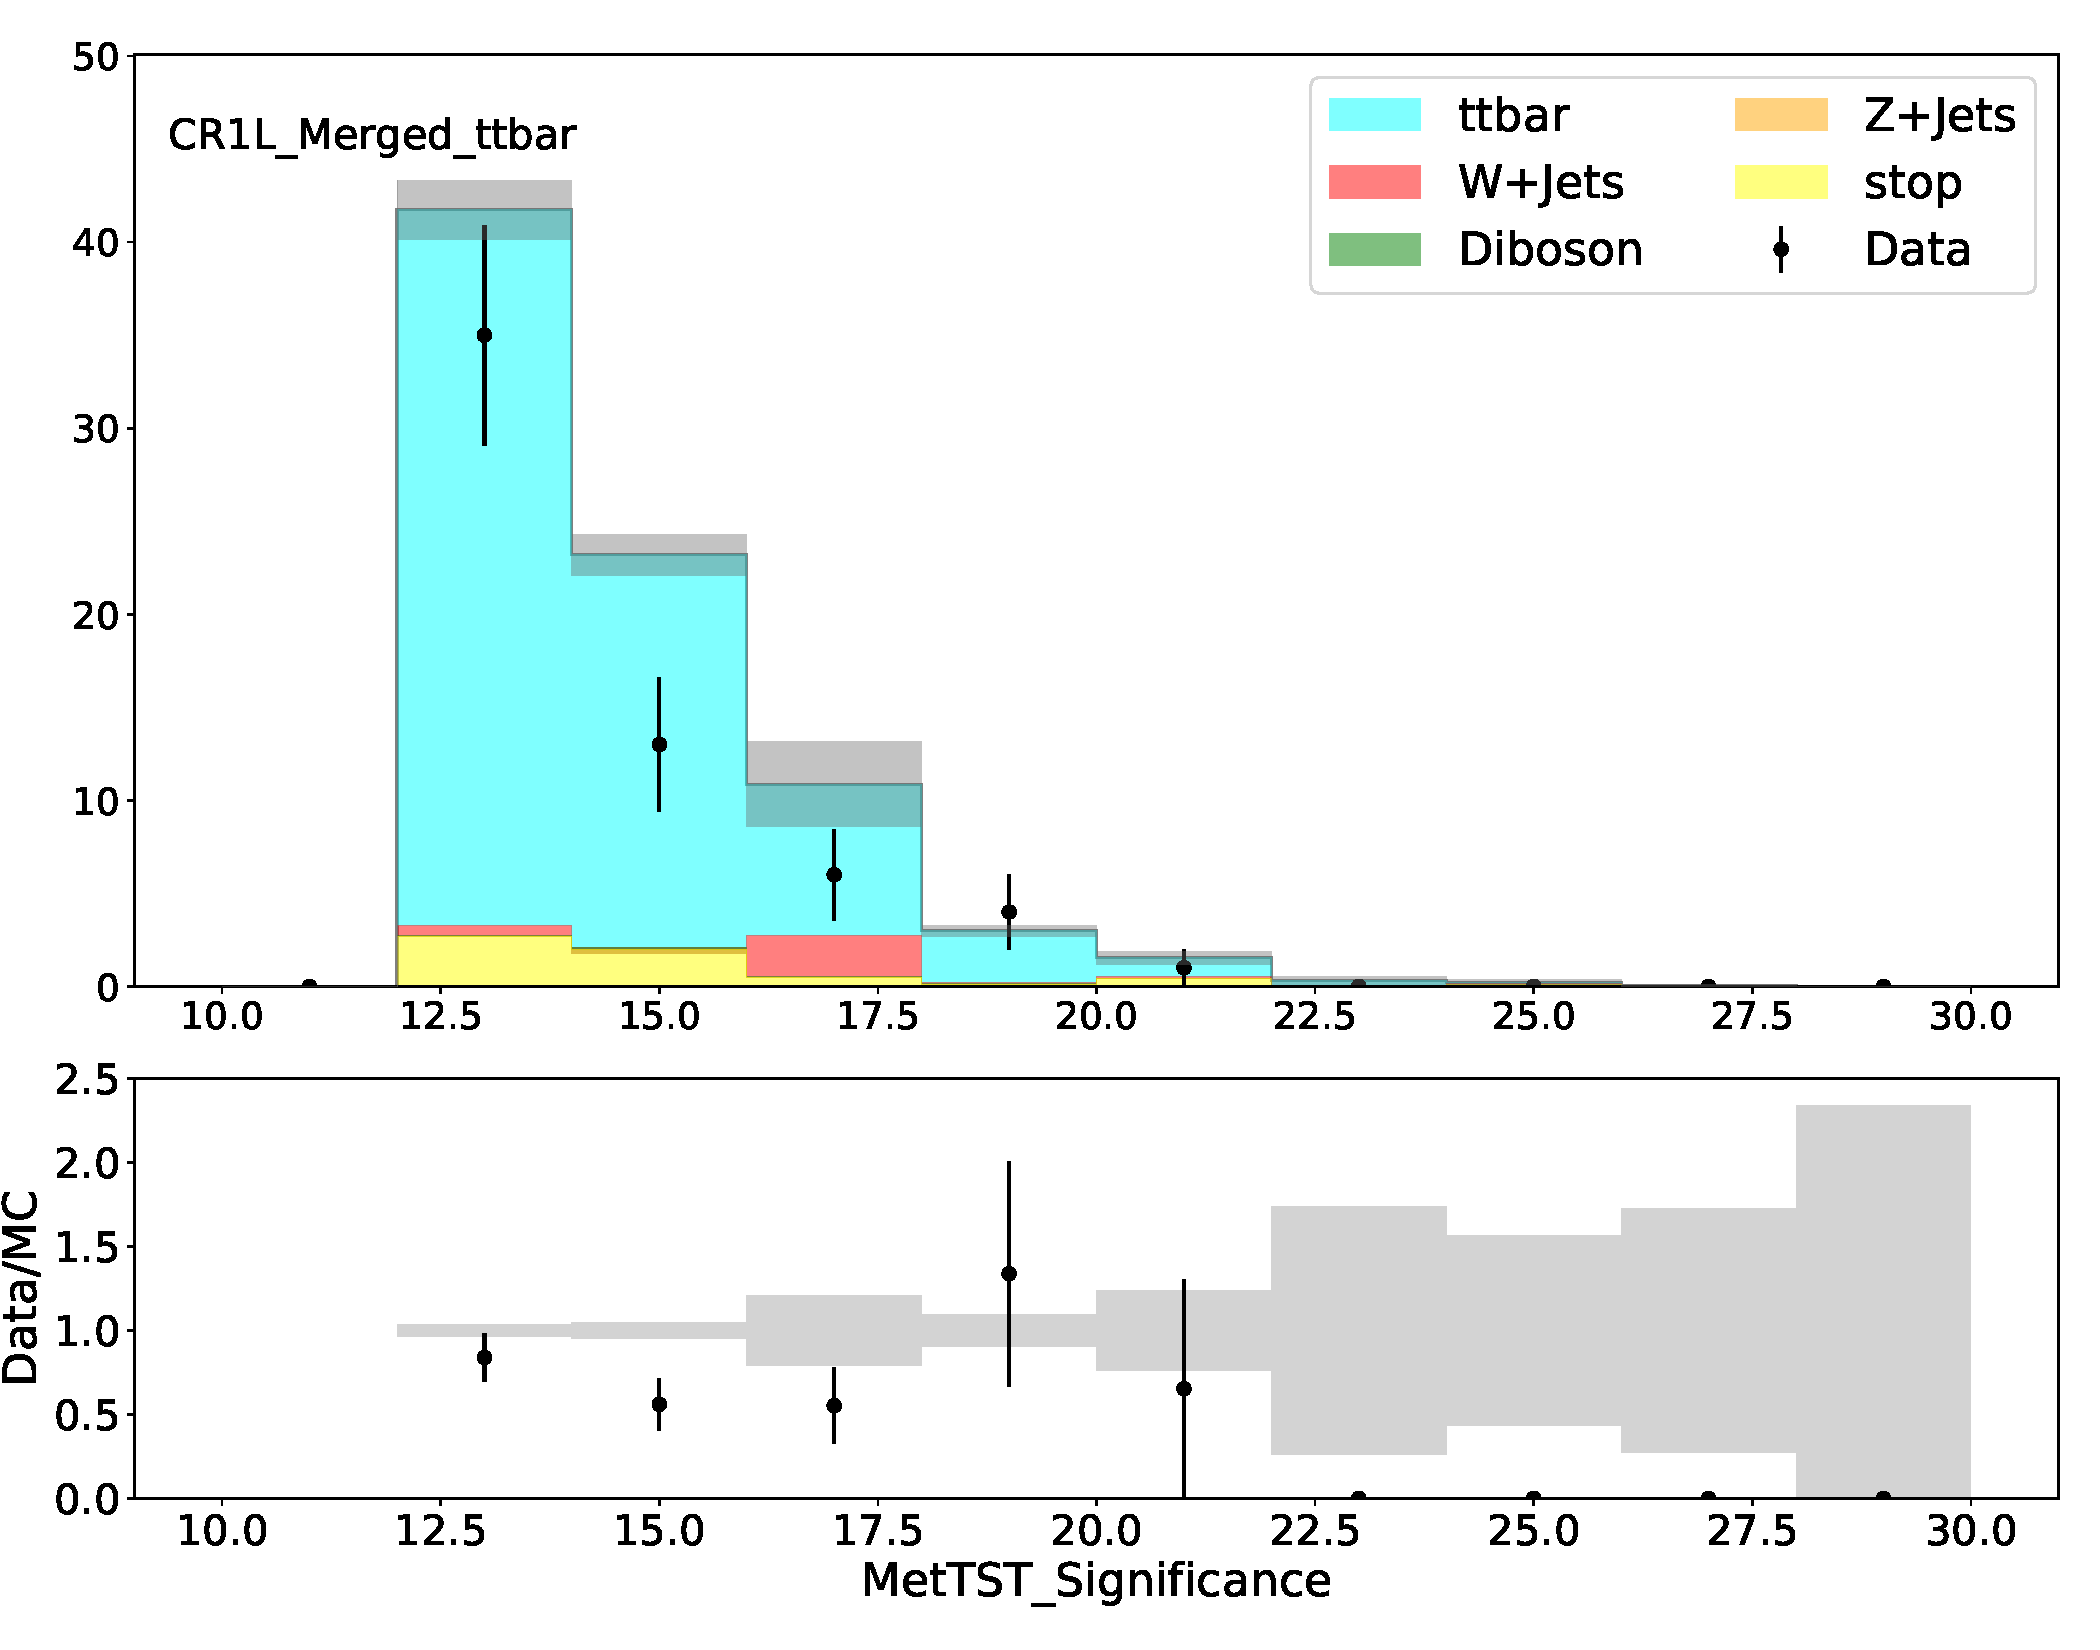
\includegraphics[width = 0.98\textwidth]{Figures/4/datamc/CR1L_Merged_ttbar/MetTST_Significance.pdf}
     \caption{\metsig}
     \end{subfigure}
     \begin{subfigure}{0.49\textwidth}
     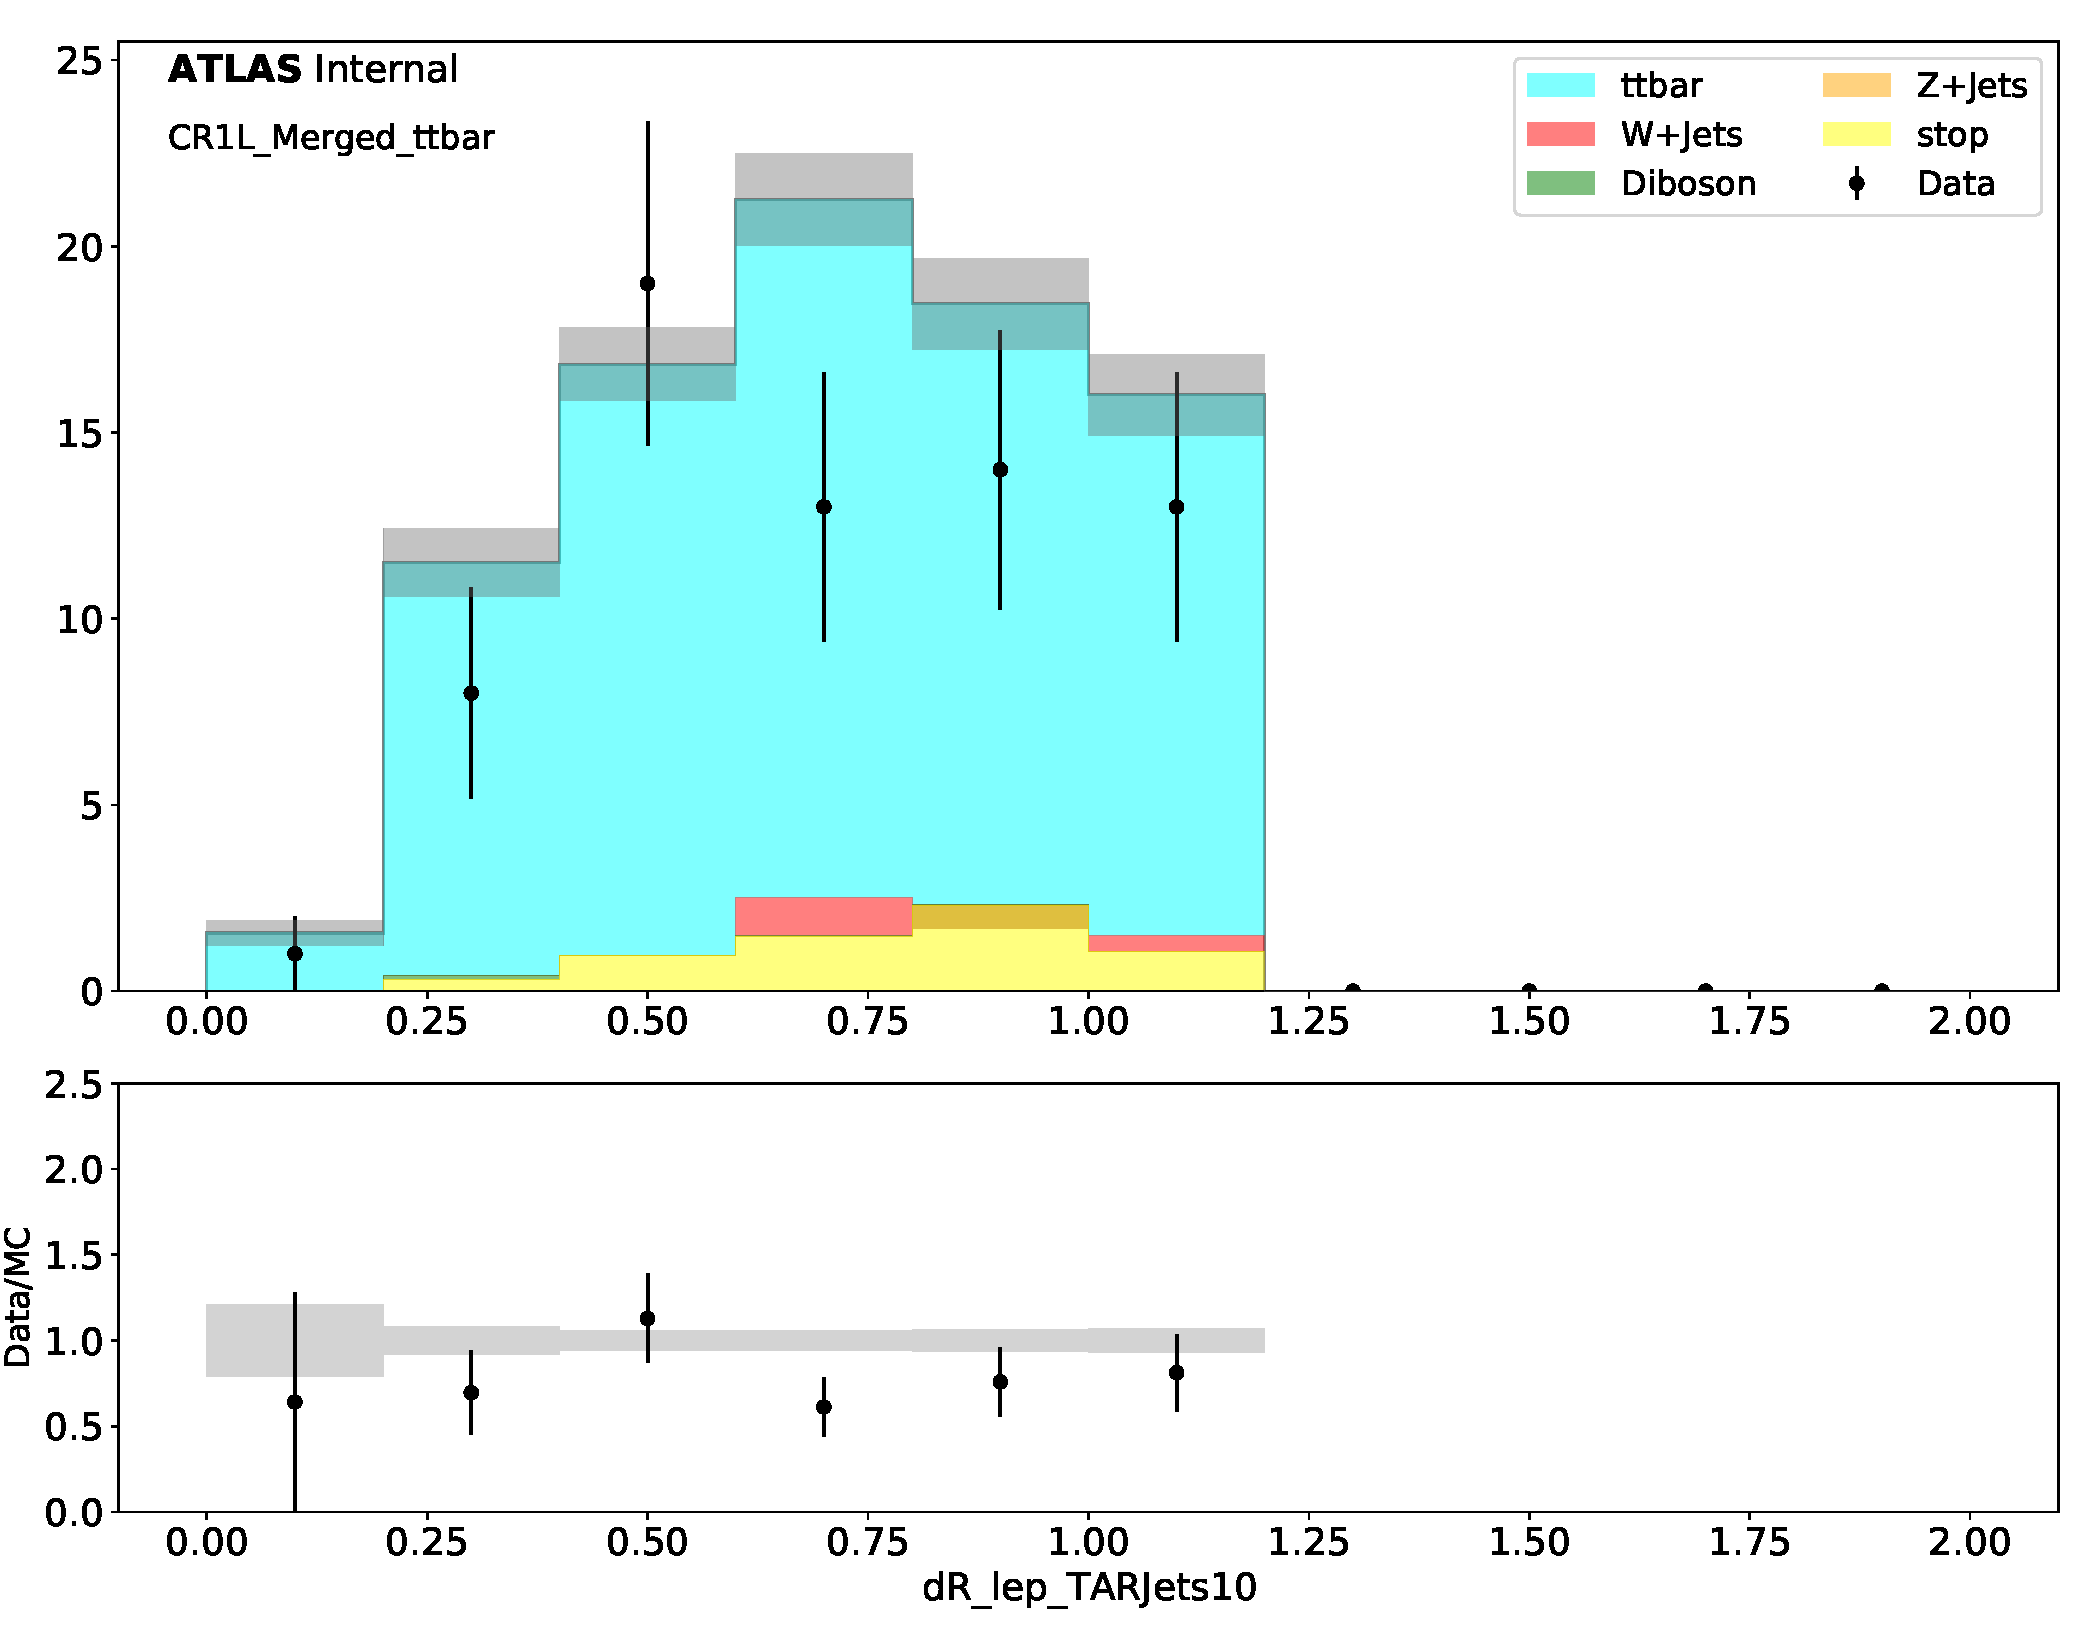
\includegraphics[width = 0.98\textwidth]{Figures/4/datamc/CR1L_Merged_ttbar/dR_lep_TARJets10.pdf}
     \caption{\drTARl}
     \end{subfigure}
     \begin{subfigure}{0.49\textwidth}
     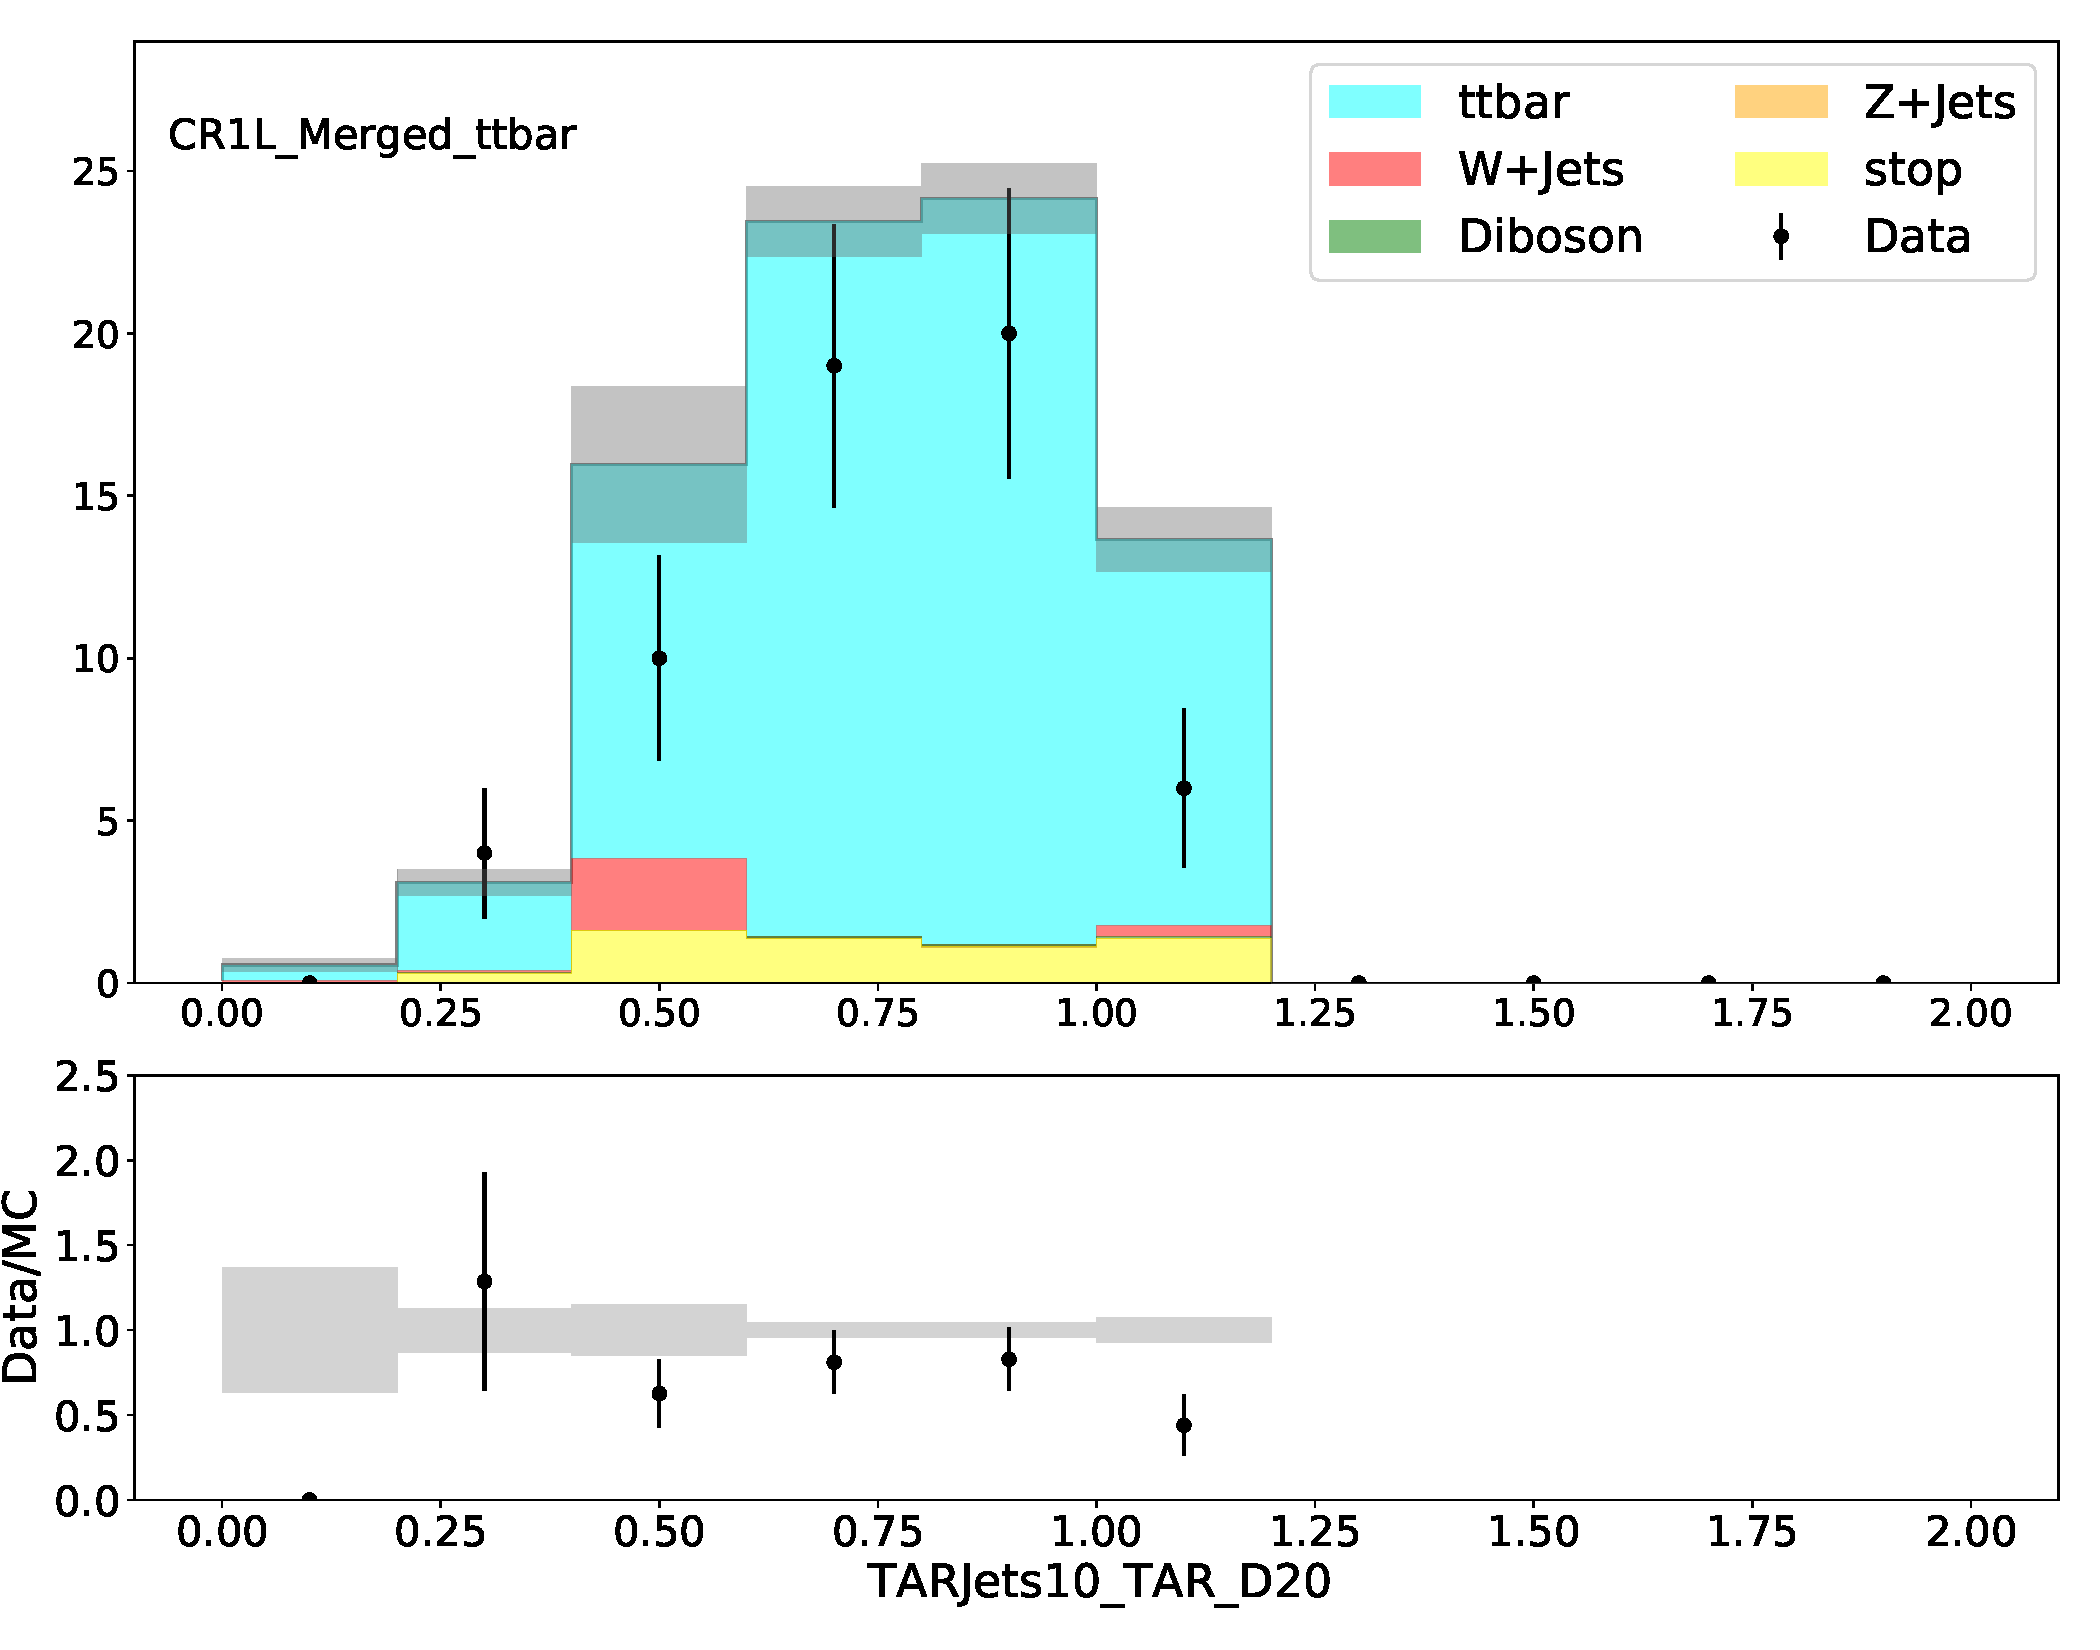
\includegraphics[width = 0.98\textwidth]{Figures/4/datamc/CR1L_Merged_ttbar/TARJets10_TAR_D20.pdf}
     \caption{\DtwoTAR}
     \end{subfigure}
     \begin{subfigure}{0.49\textwidth}
     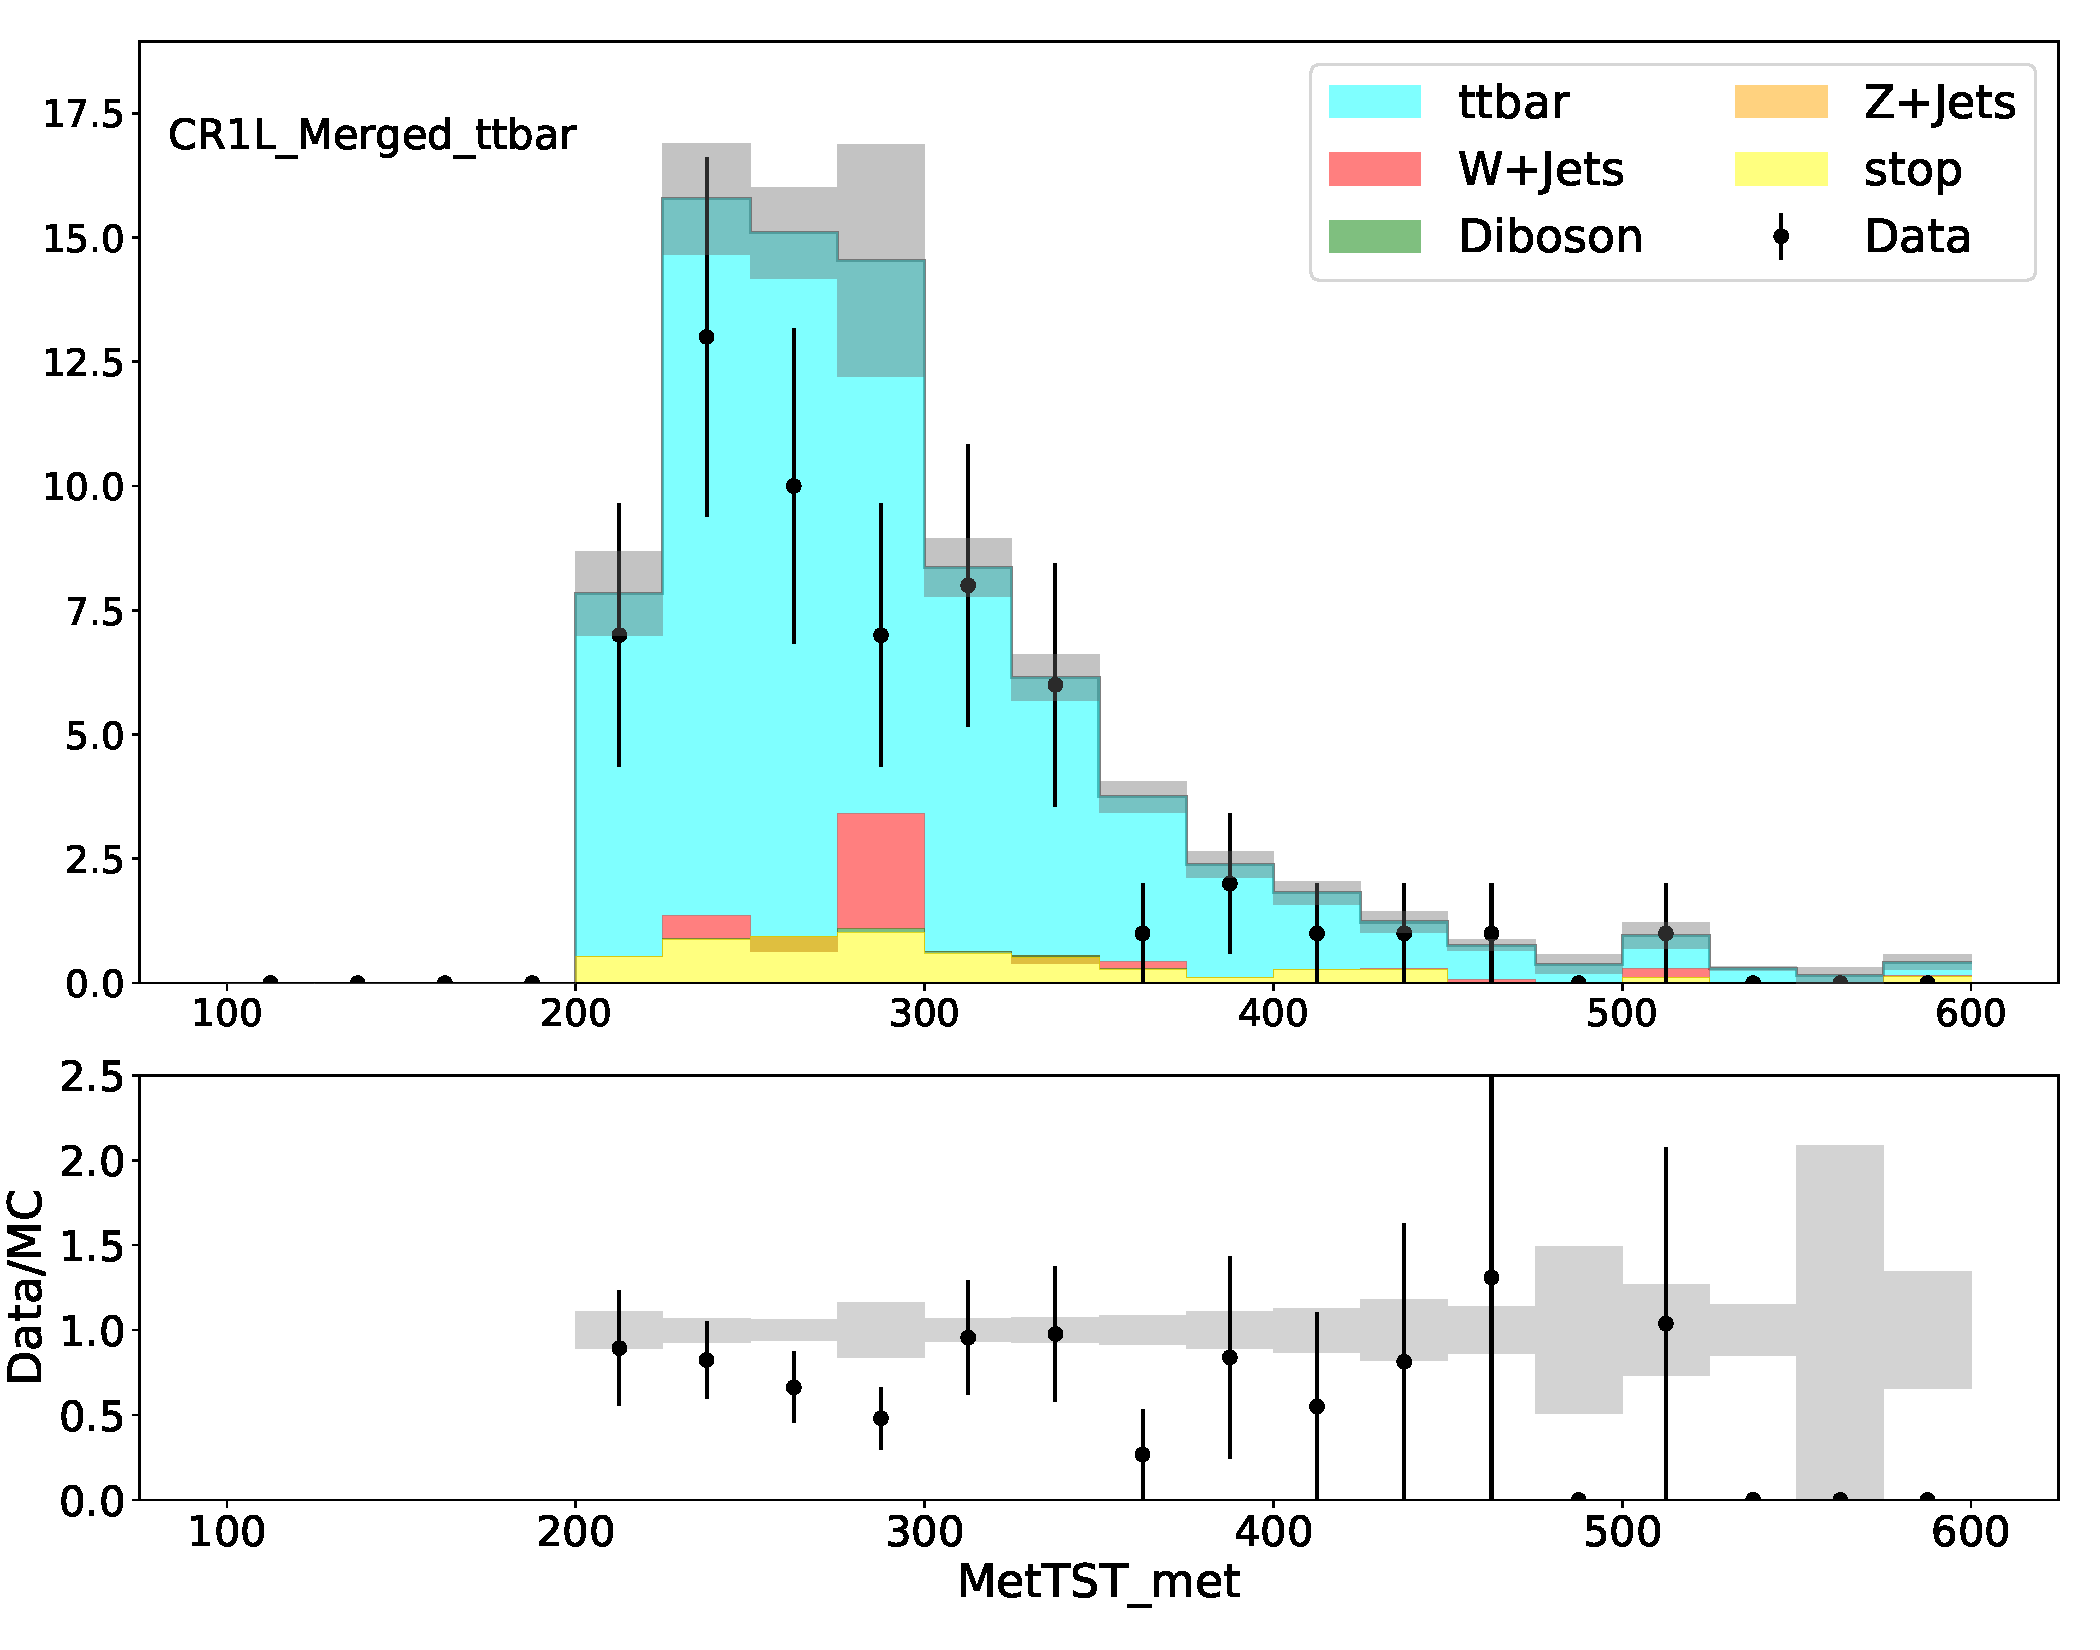
\includegraphics[width = 0.98\textwidth]{Figures/4/datamc/CR1L_Merged_ttbar/MetTST_met.pdf}
     \caption{\met}
     \end{subfigure}

     \caption{Data-MC Comparisons in the \merged \ttbar control region}
     \label{fig:Data_MC_CRbV_merged}
  \end{figure}

\begin{figure}[htbp]
  \centering
     \begin{subfigure}{0.49\textwidth}
     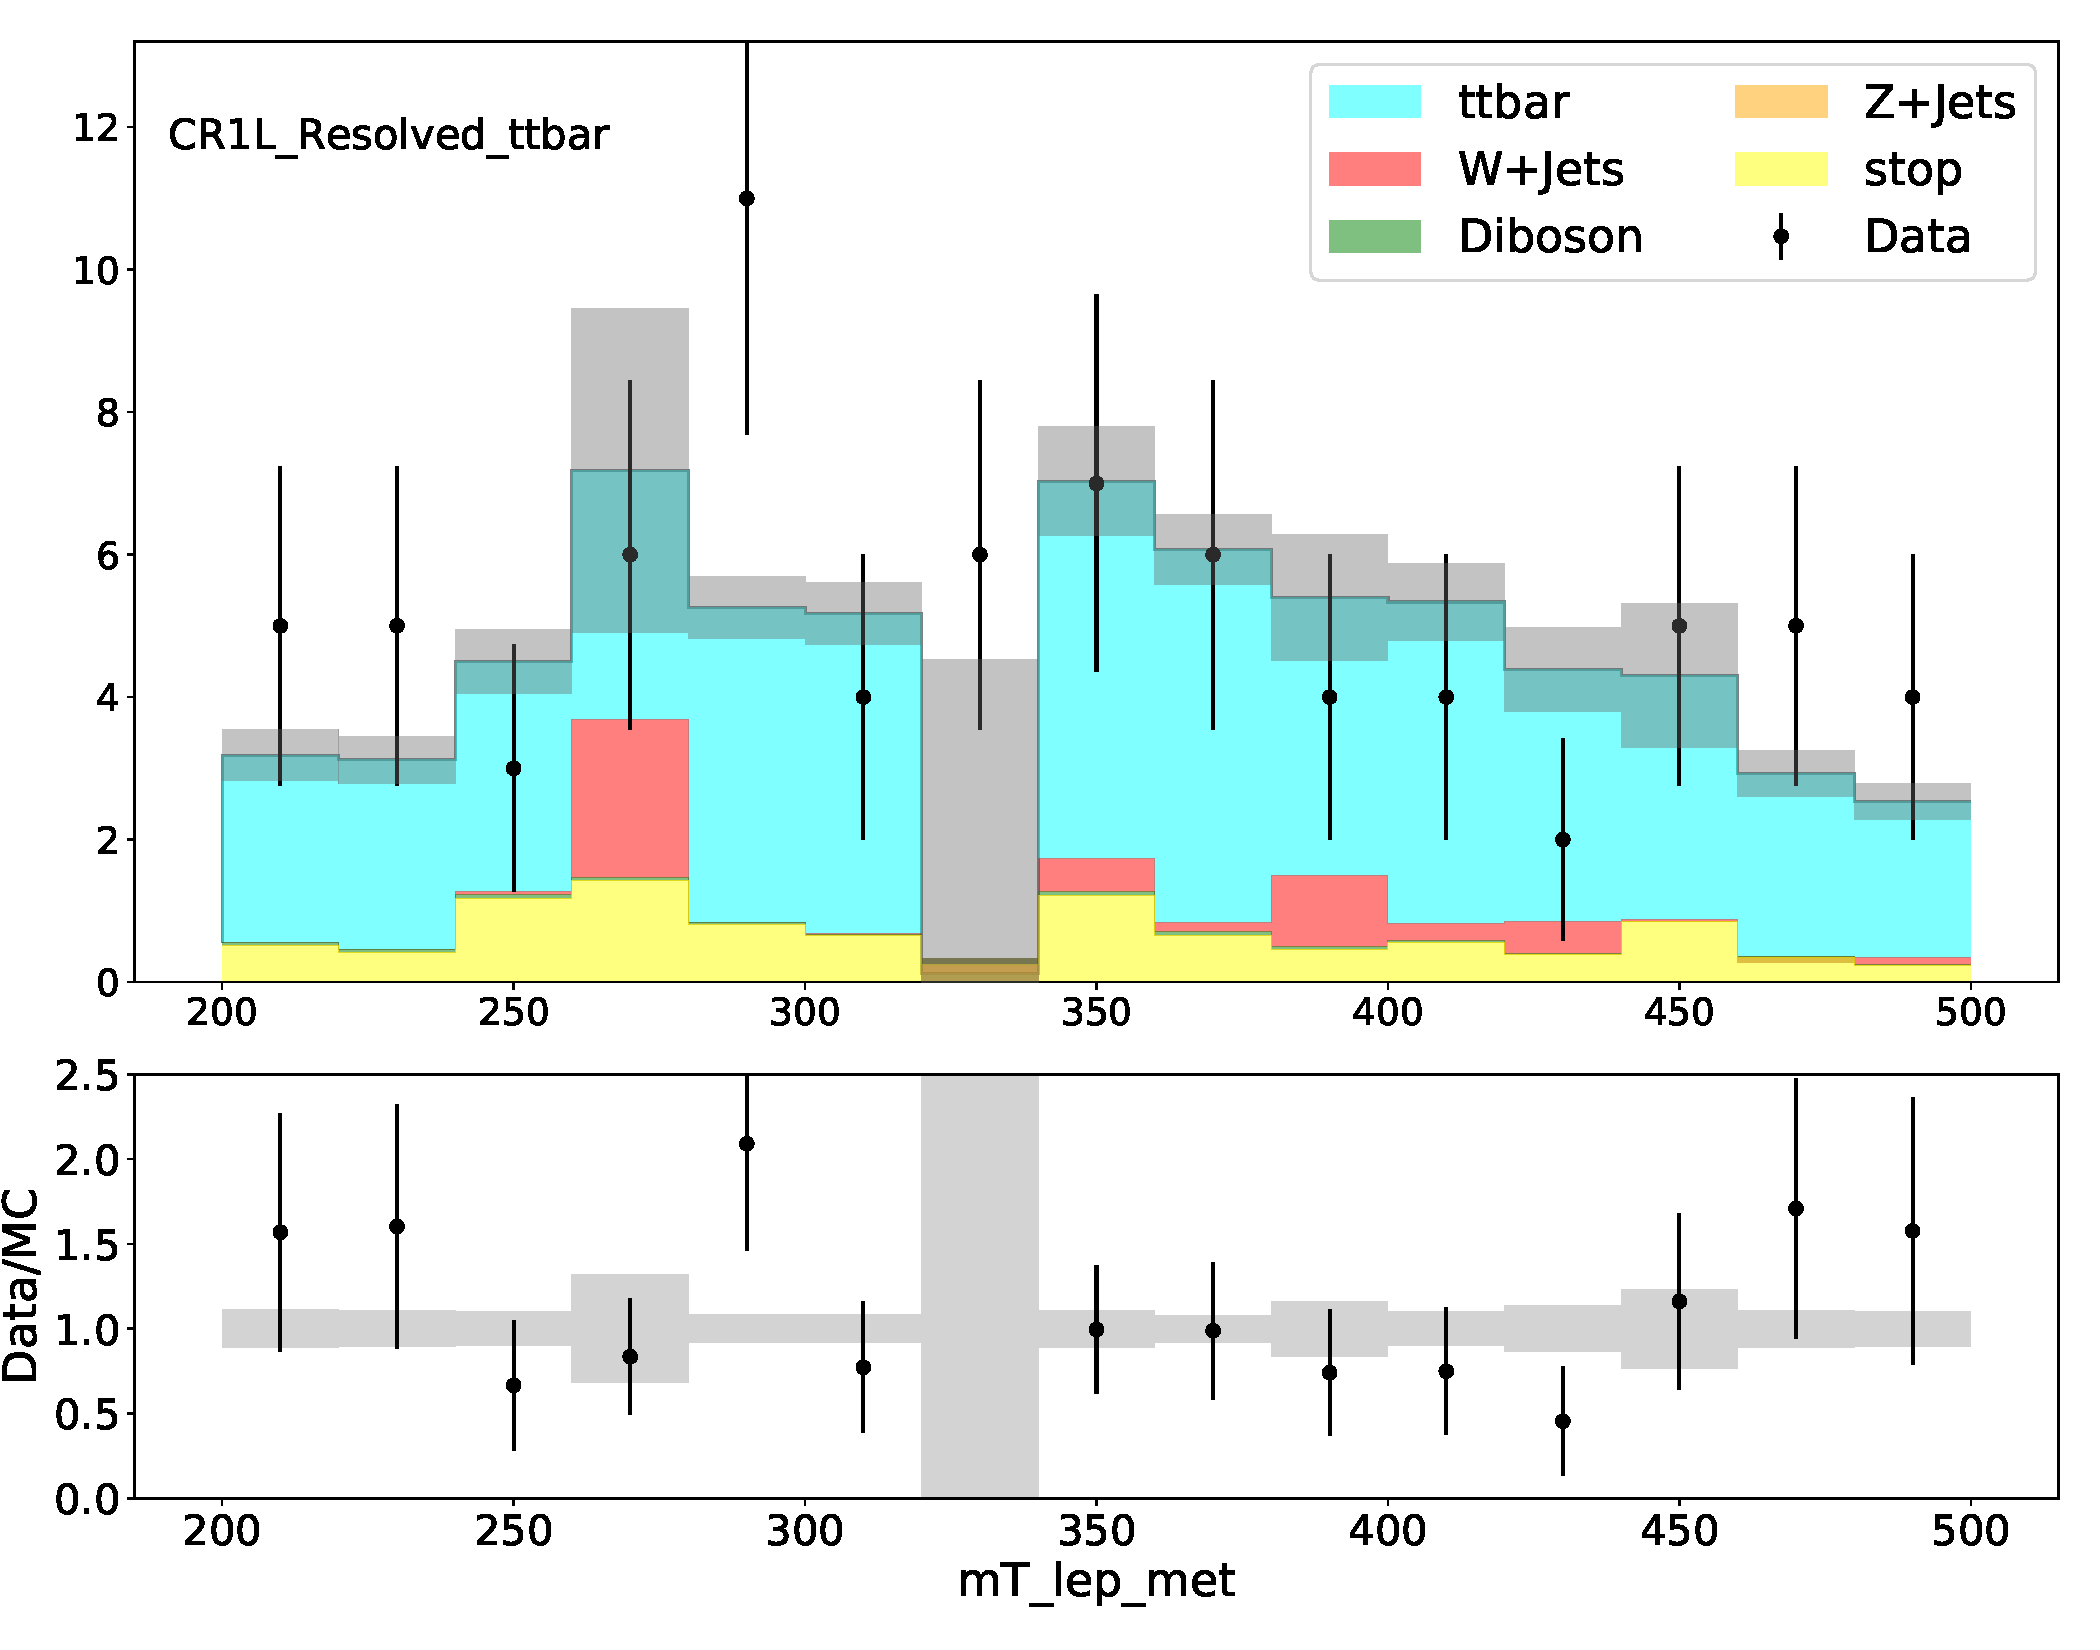
\includegraphics[width = 0.98\textwidth]{Figures/4/datamc/CR1L_Resolved_ttbar/mT_lep_met.pdf}
     \caption{\mtlepmet}
     \end{subfigure}
     \begin{subfigure}{0.49\textwidth}
     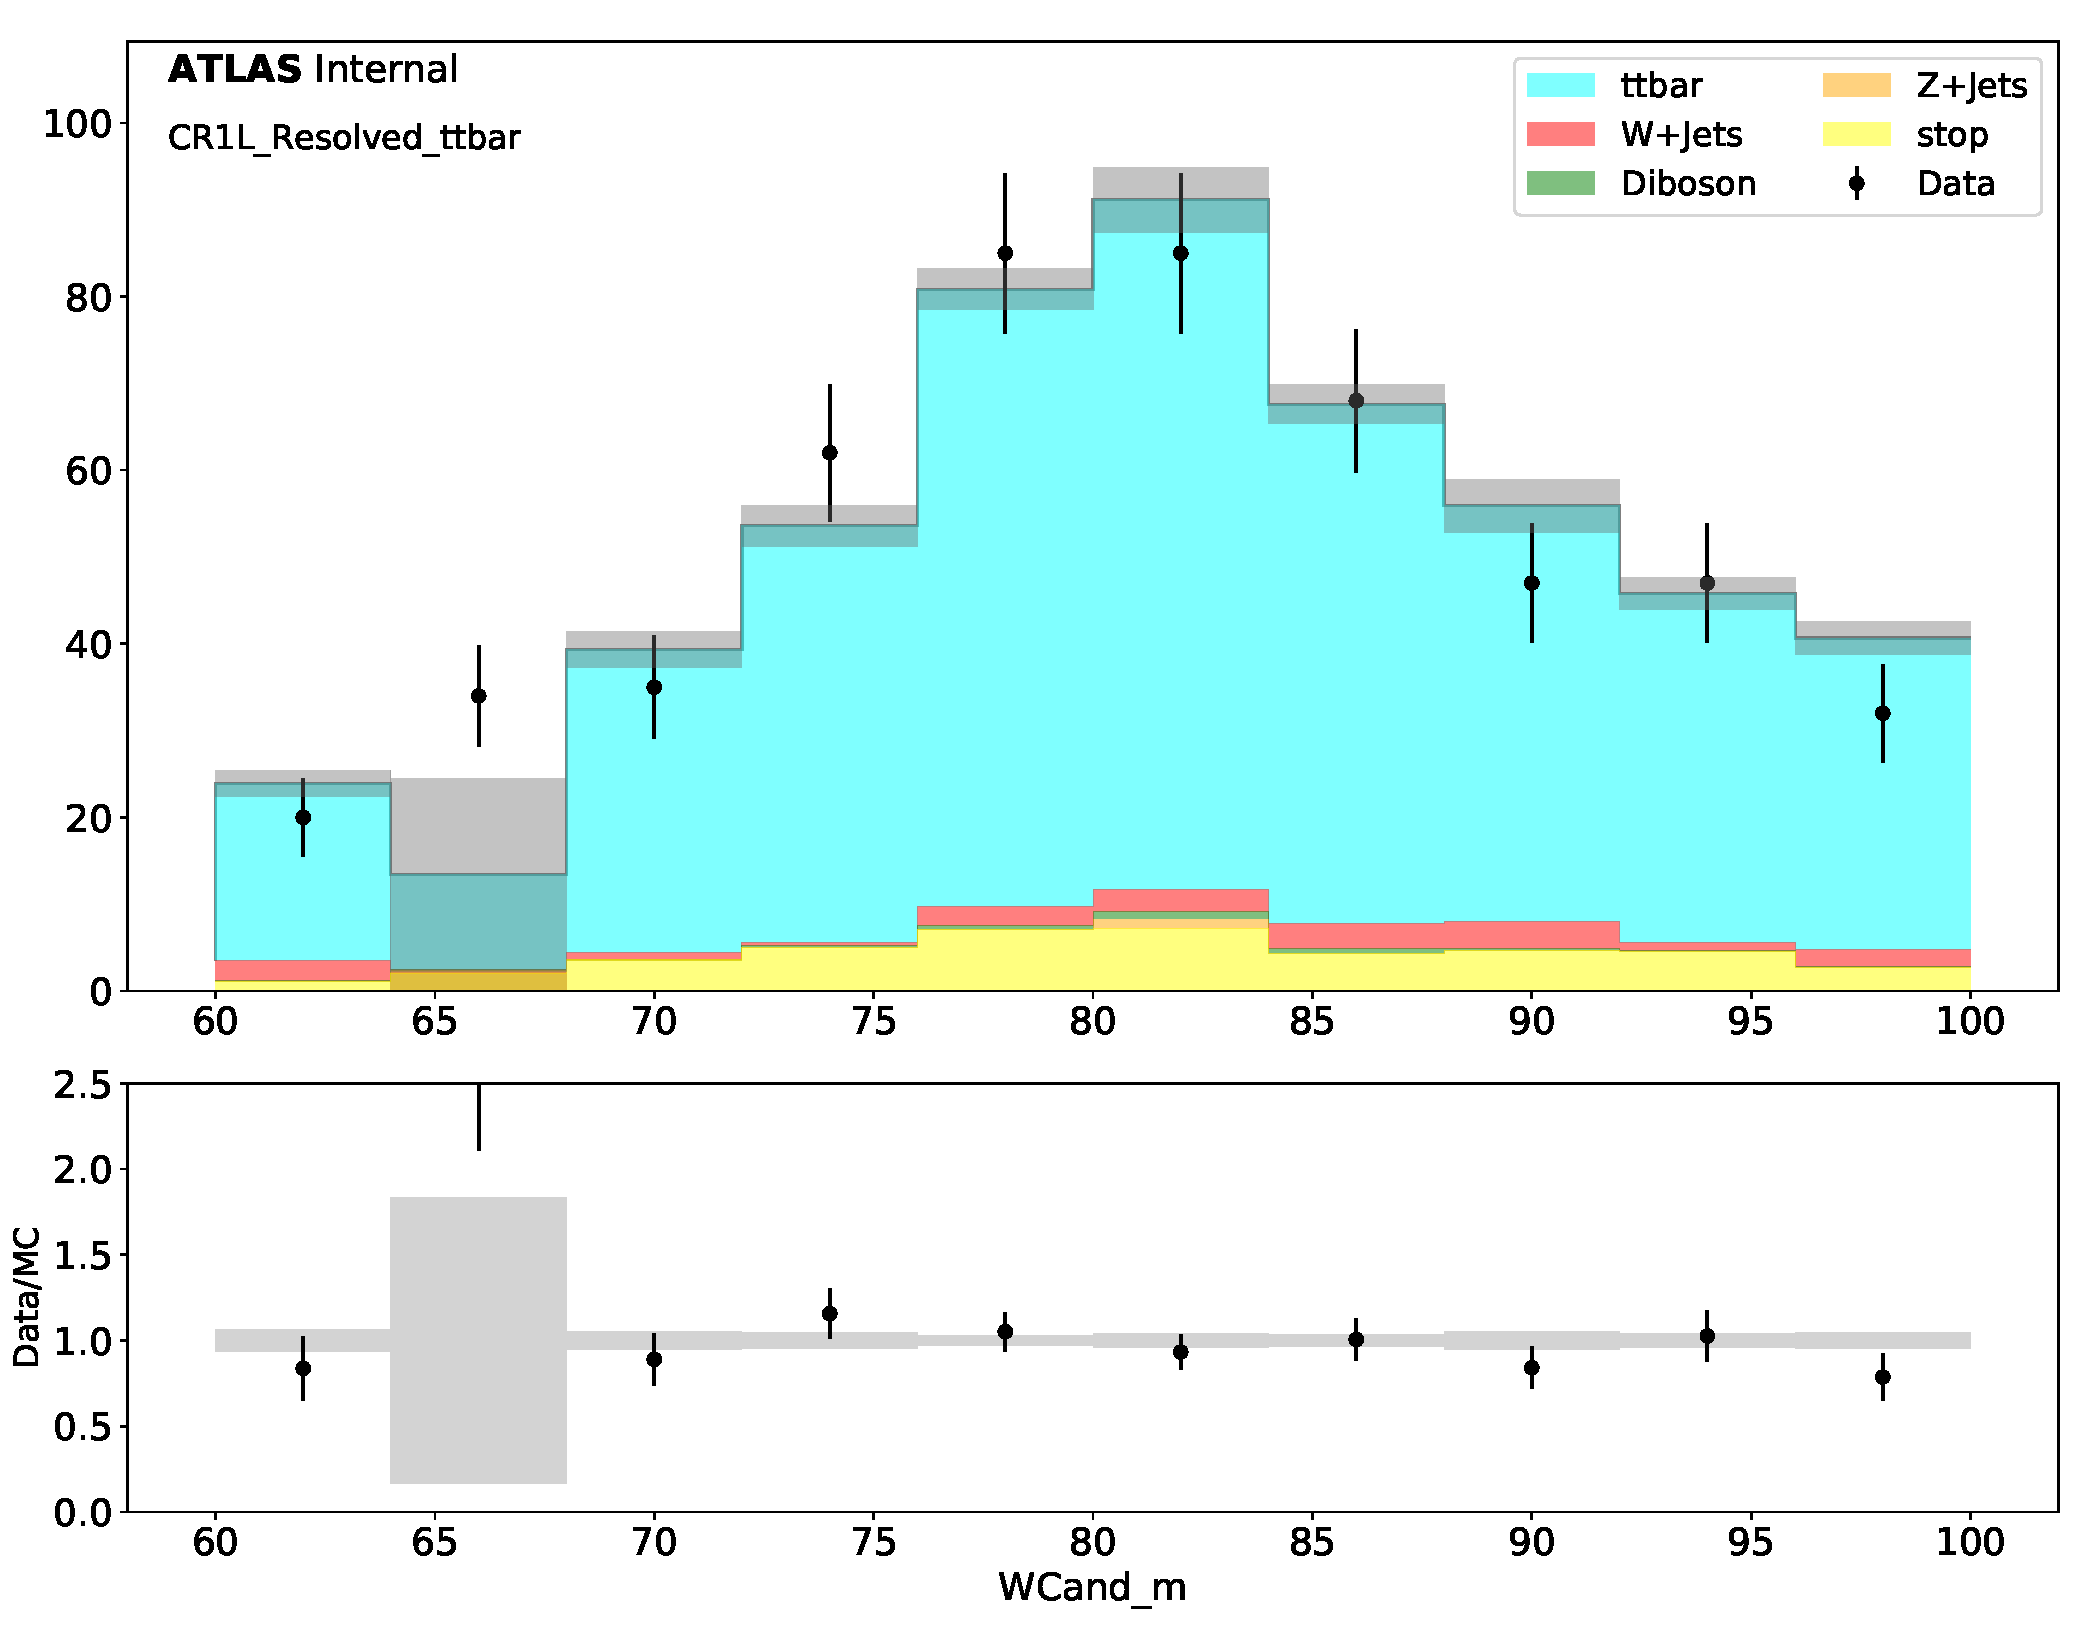
\includegraphics[width = 0.98\textwidth]{Figures/4/datamc/CR1L_Resolved_ttbar/WCand_m.pdf}
     \caption{\Wcandm}
     \end{subfigure}
     \begin{subfigure}{0.49\textwidth}
     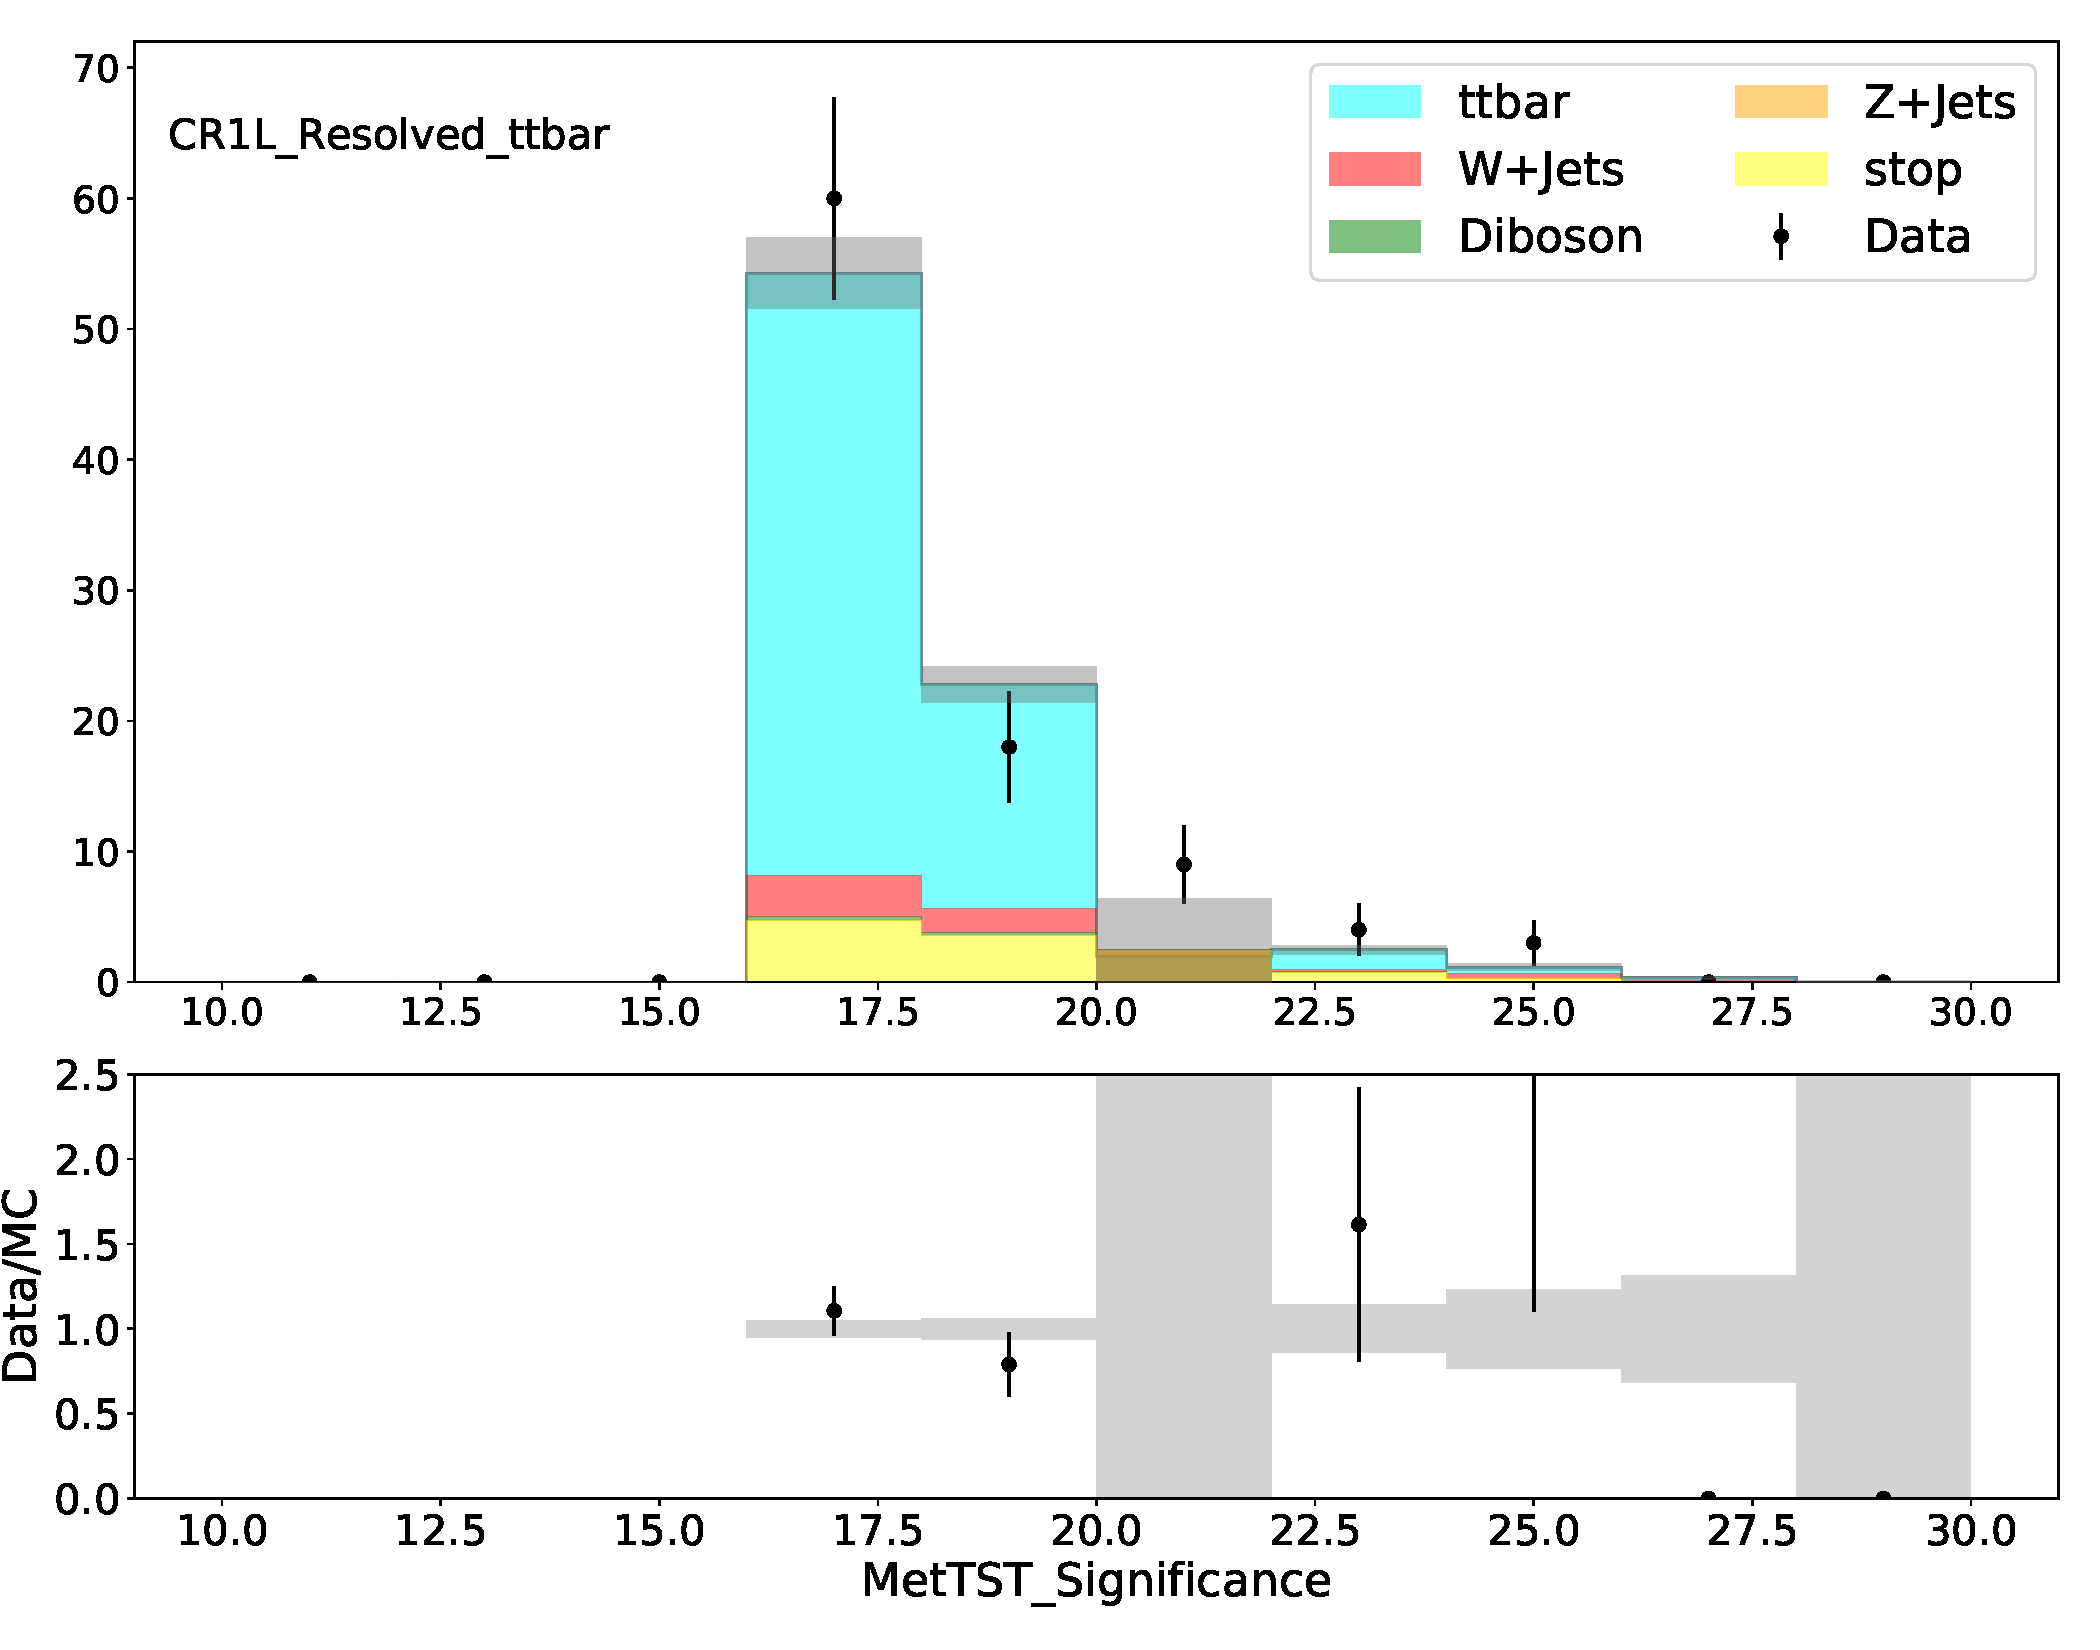
\includegraphics[width = 0.98\textwidth]{Figures/4/datamc/CR1L_Resolved_ttbar/MetTST_Significance.pdf}
     \caption{\metsig}
     \end{subfigure}
     \begin{subfigure}{0.49\textwidth}
     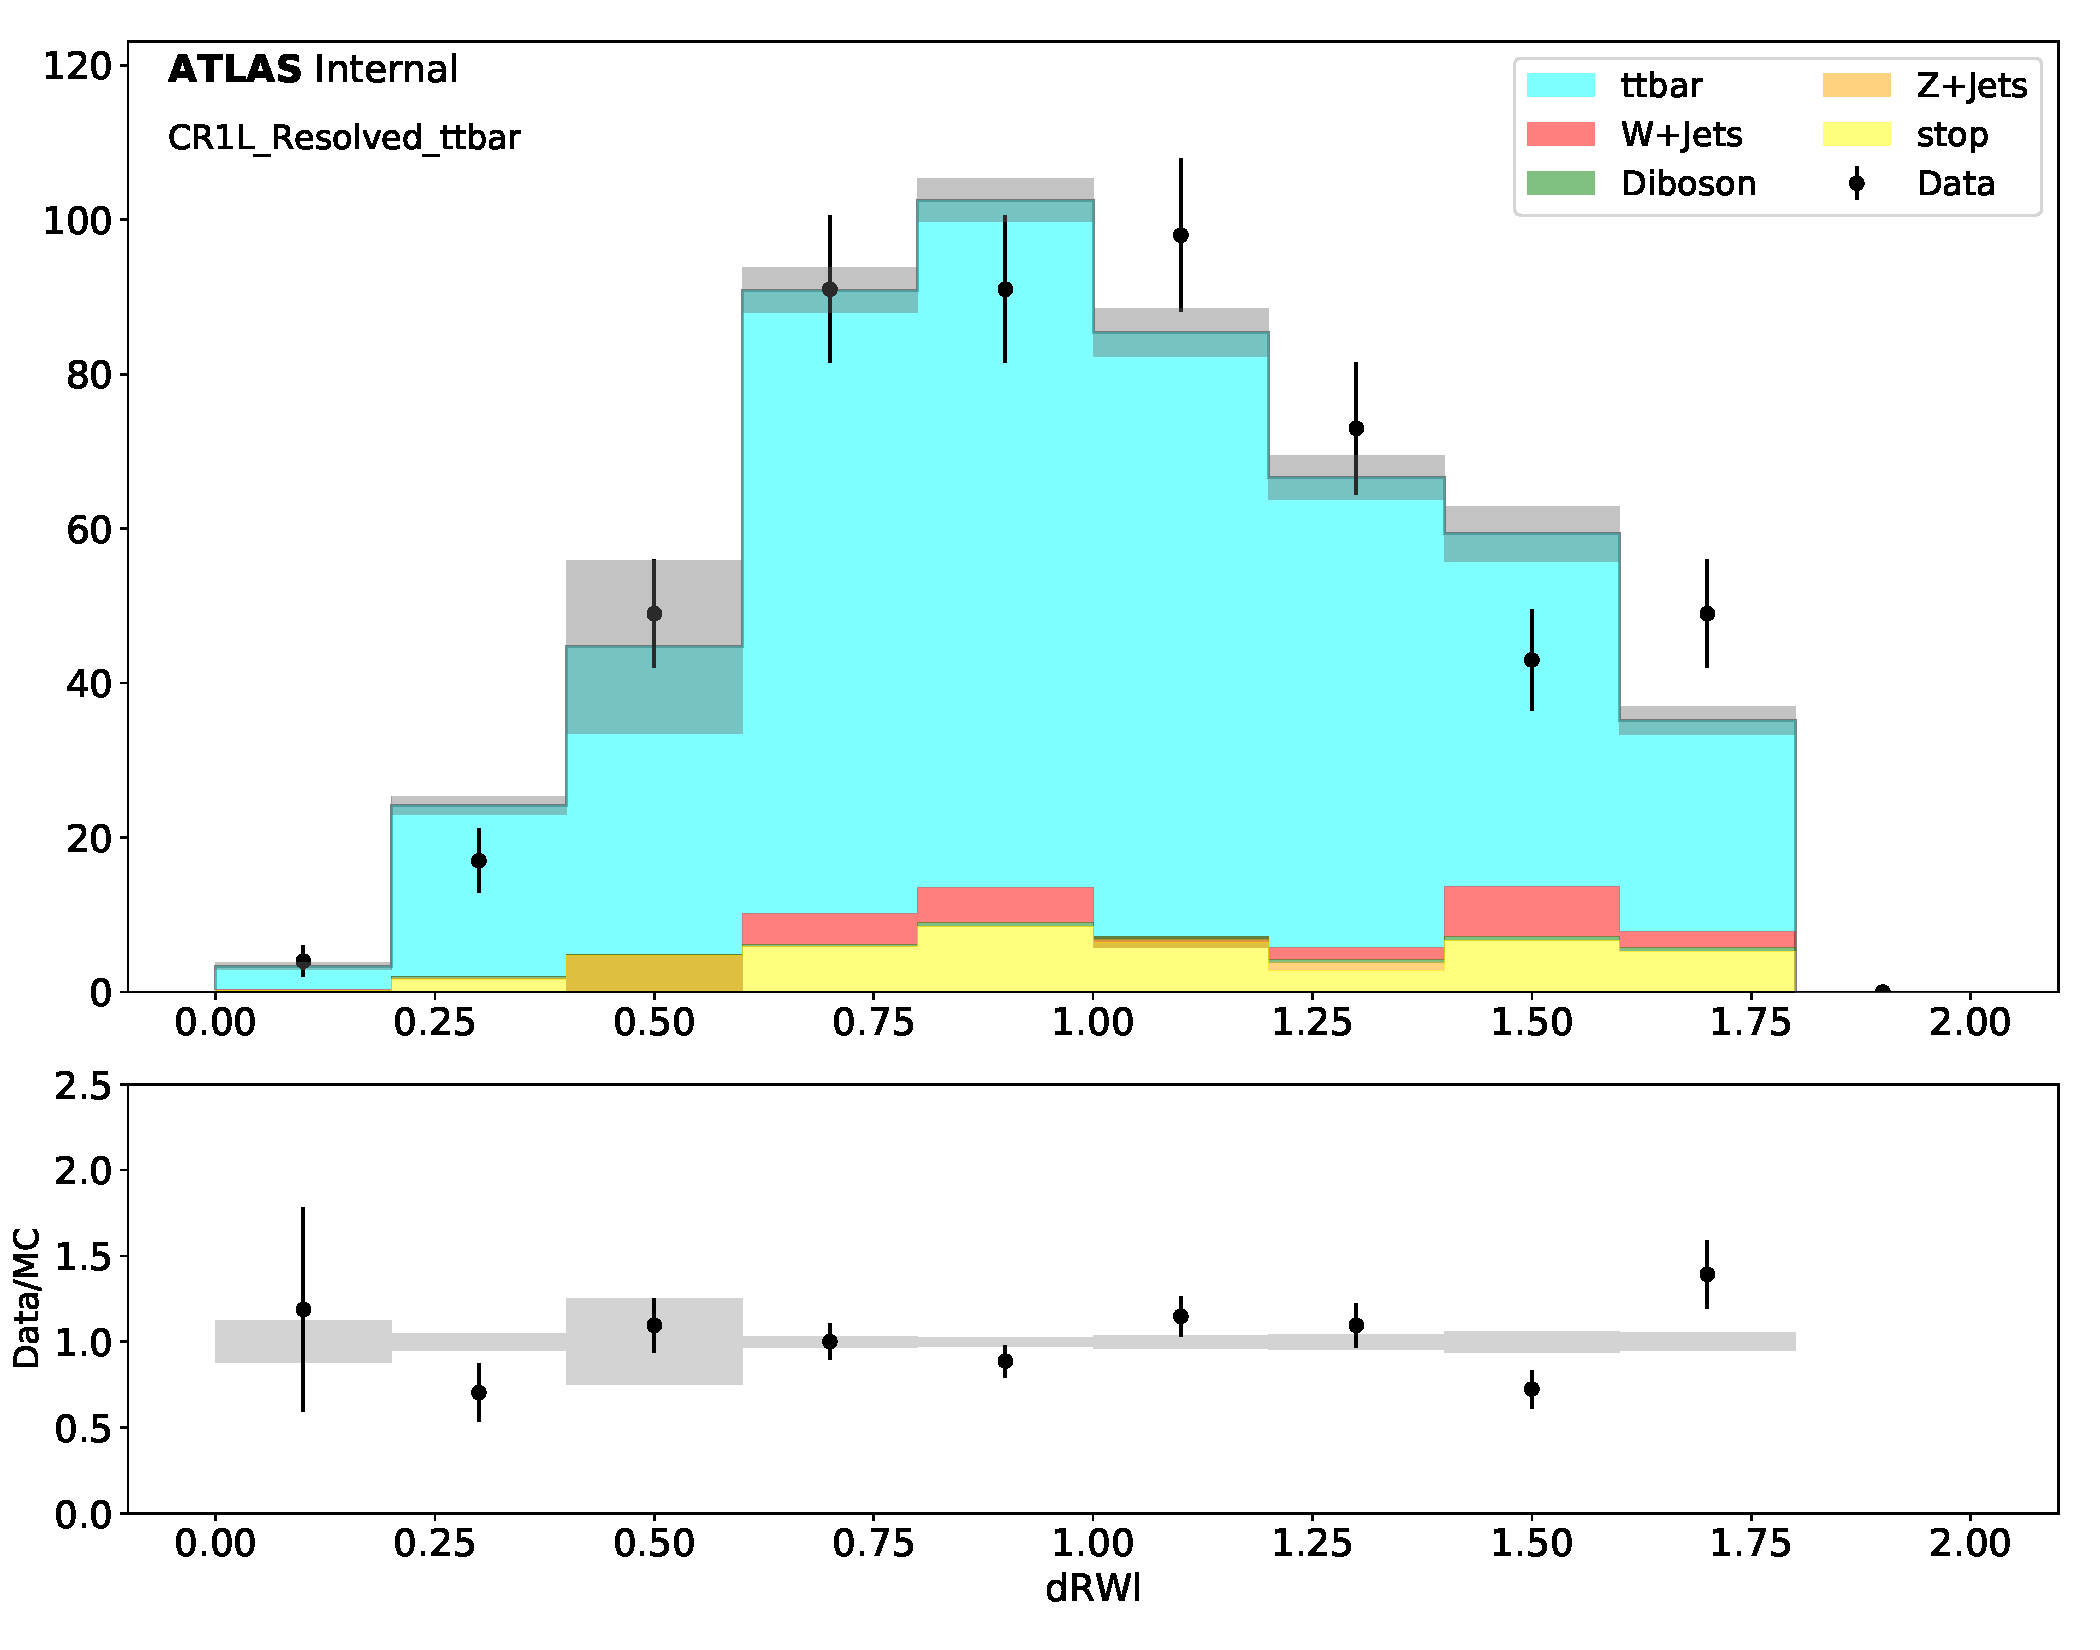
\includegraphics[width = 0.98\textwidth]{Figures/4/datamc/CR1L_Resolved_ttbar/dRWl.pdf}
     \caption{\drWl}
     \end{subfigure}
     \begin{subfigure}{0.49\textwidth}
     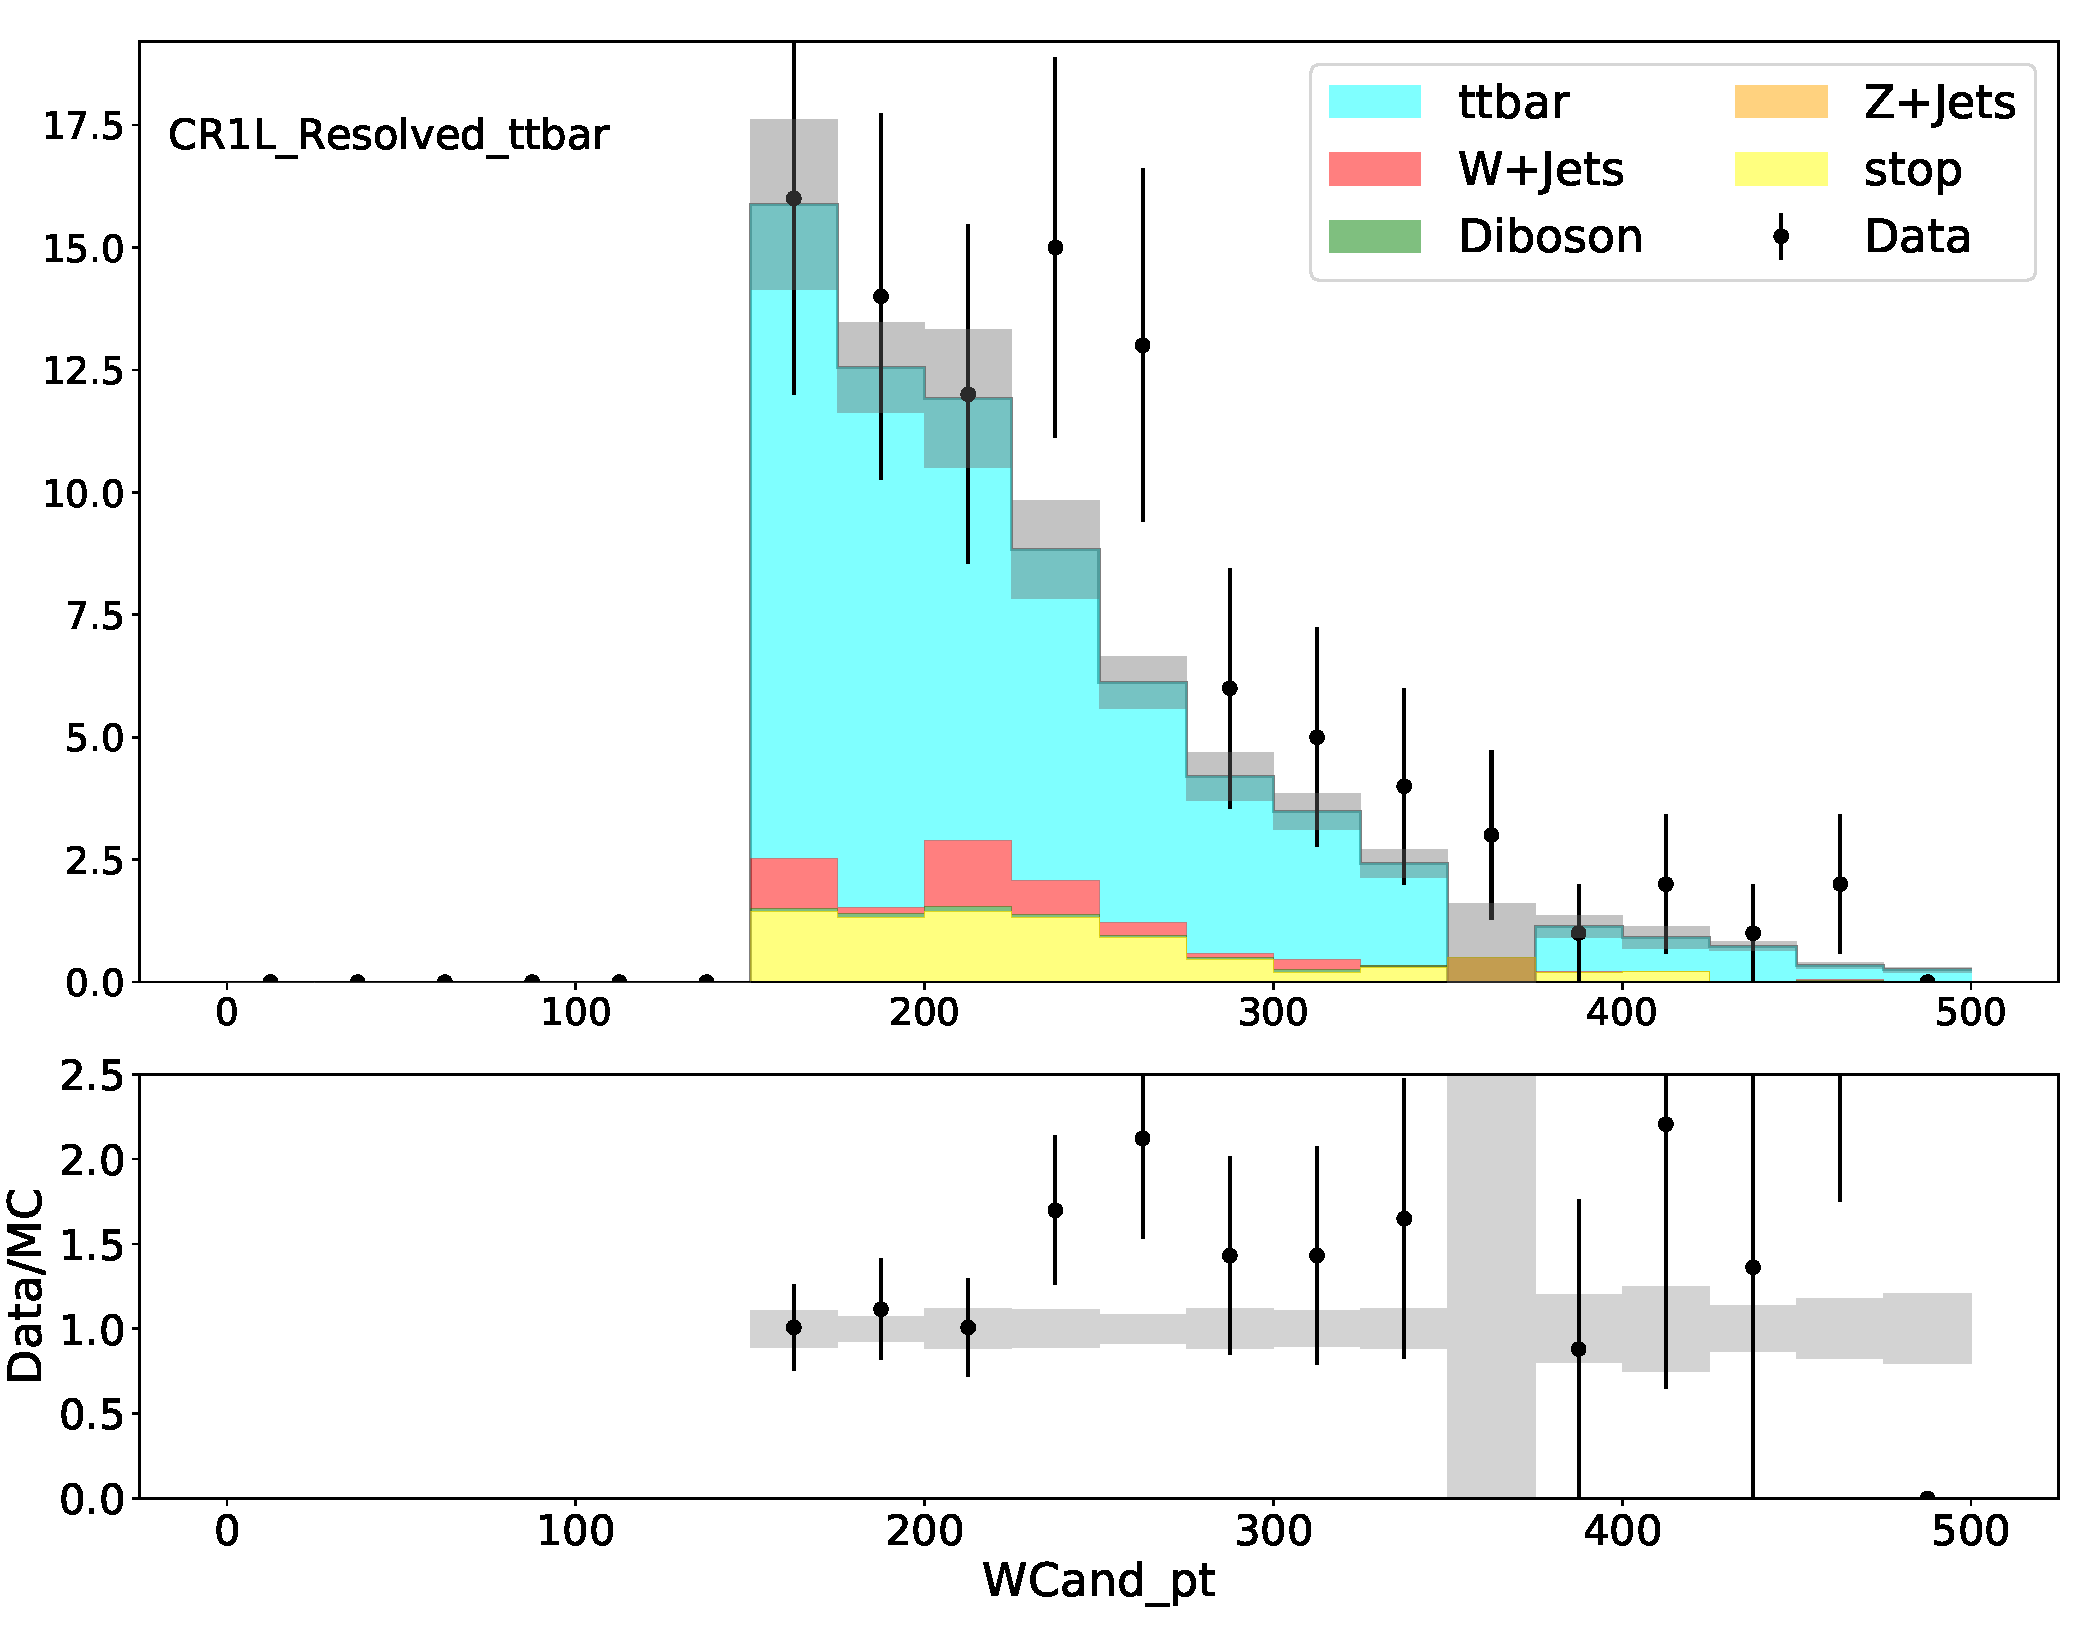
\includegraphics[width = 0.98\textwidth]{Figures/4/datamc/CR1L_Resolved_ttbar/WCand_pt.pdf}
     \caption{\Wcandpt}
     \end{subfigure}
     \begin{subfigure}{0.49\textwidth}
     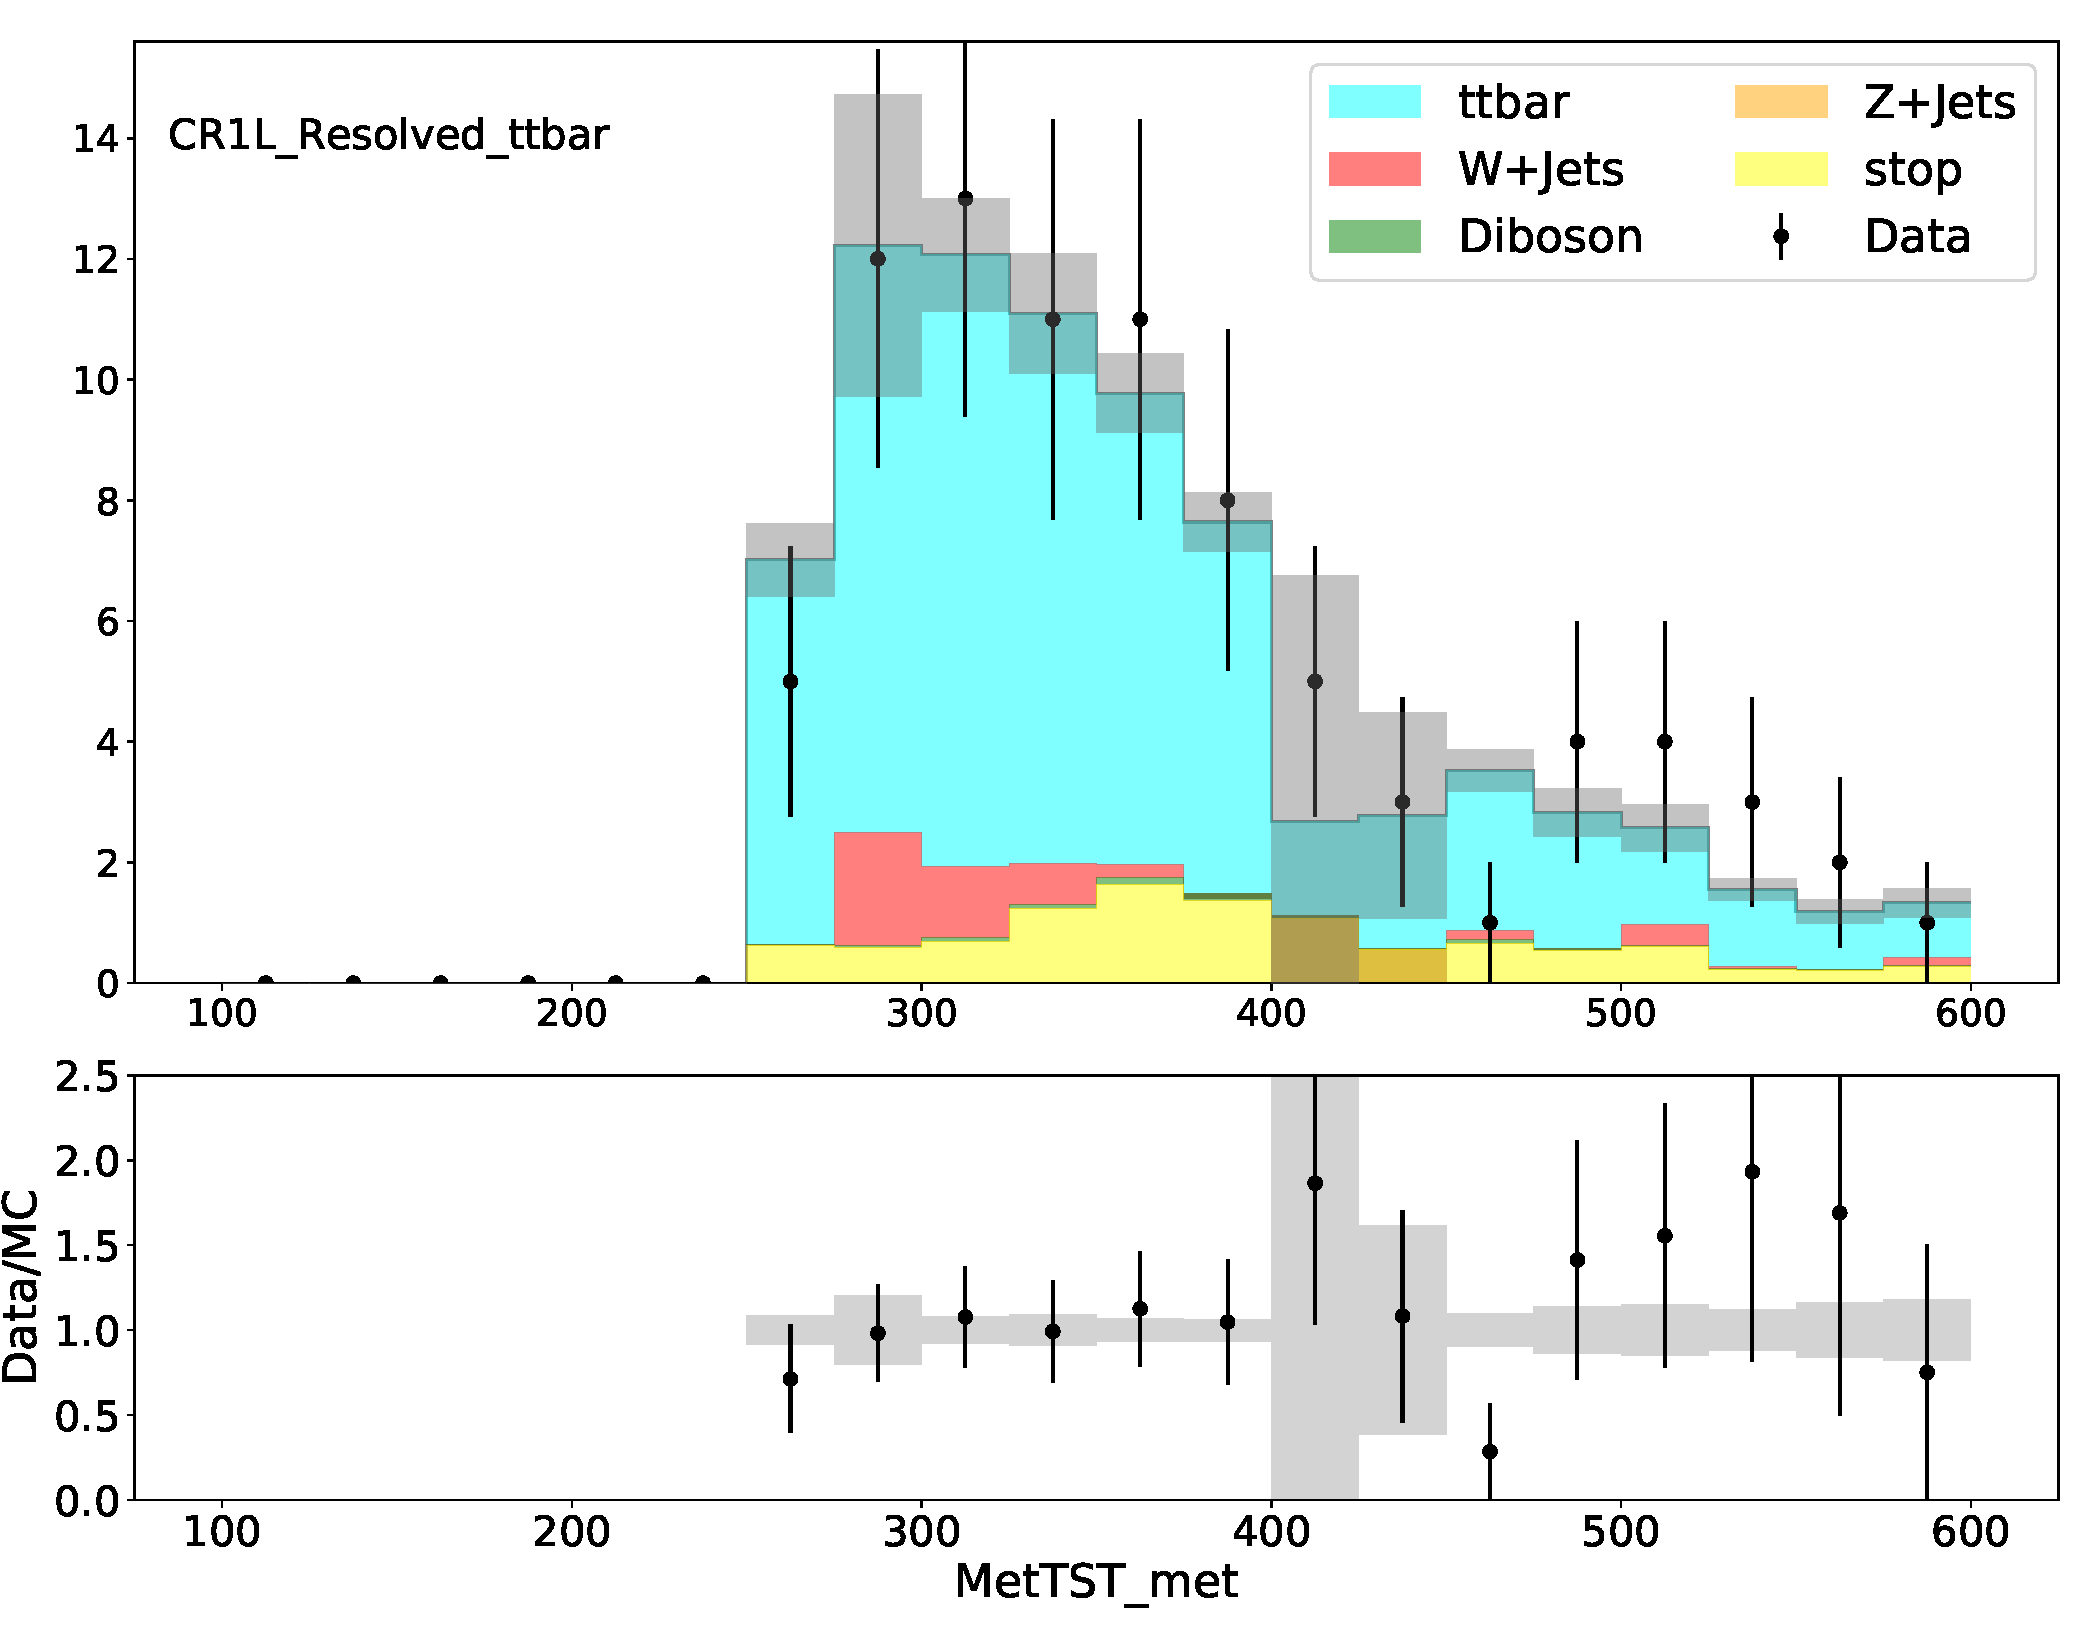
\includegraphics[width = 0.98\textwidth]{Figures/4/datamc/CR1L_Resolved_ttbar/MetTST_met.pdf}
     \caption{\met}
     \end{subfigure}

\caption{Data-MC Comparisons in the \resolved \ttbar control region}
\label{fig:Data_MC_CRbV_resolved}
\end{figure}


\section{\wjets Control Region}
An additional pair of control regions are defined in order to constrain the dominant \wjets background in the signa regions. These regions are defined by reversing the \drTARl and \drWl cuts in the \merged and \resolved signal regions. This reverses the position of the neutrino and charged lepton in the $W$ decay without substantially altering the remaining kinematics of the event that allow the hadronic activity to fake a second $W$. In the \merged \wjets control region the \metsig cut is reduced to \metsig > 12 in order to improve statistical power.

Table ~ summarizes the differences in selection criteria between the \merged and \resolved signal and \wjets control regions.

\begin{figure}[htbp]
  \centering
     \begin{subfigure}{0.49\textwidth}
     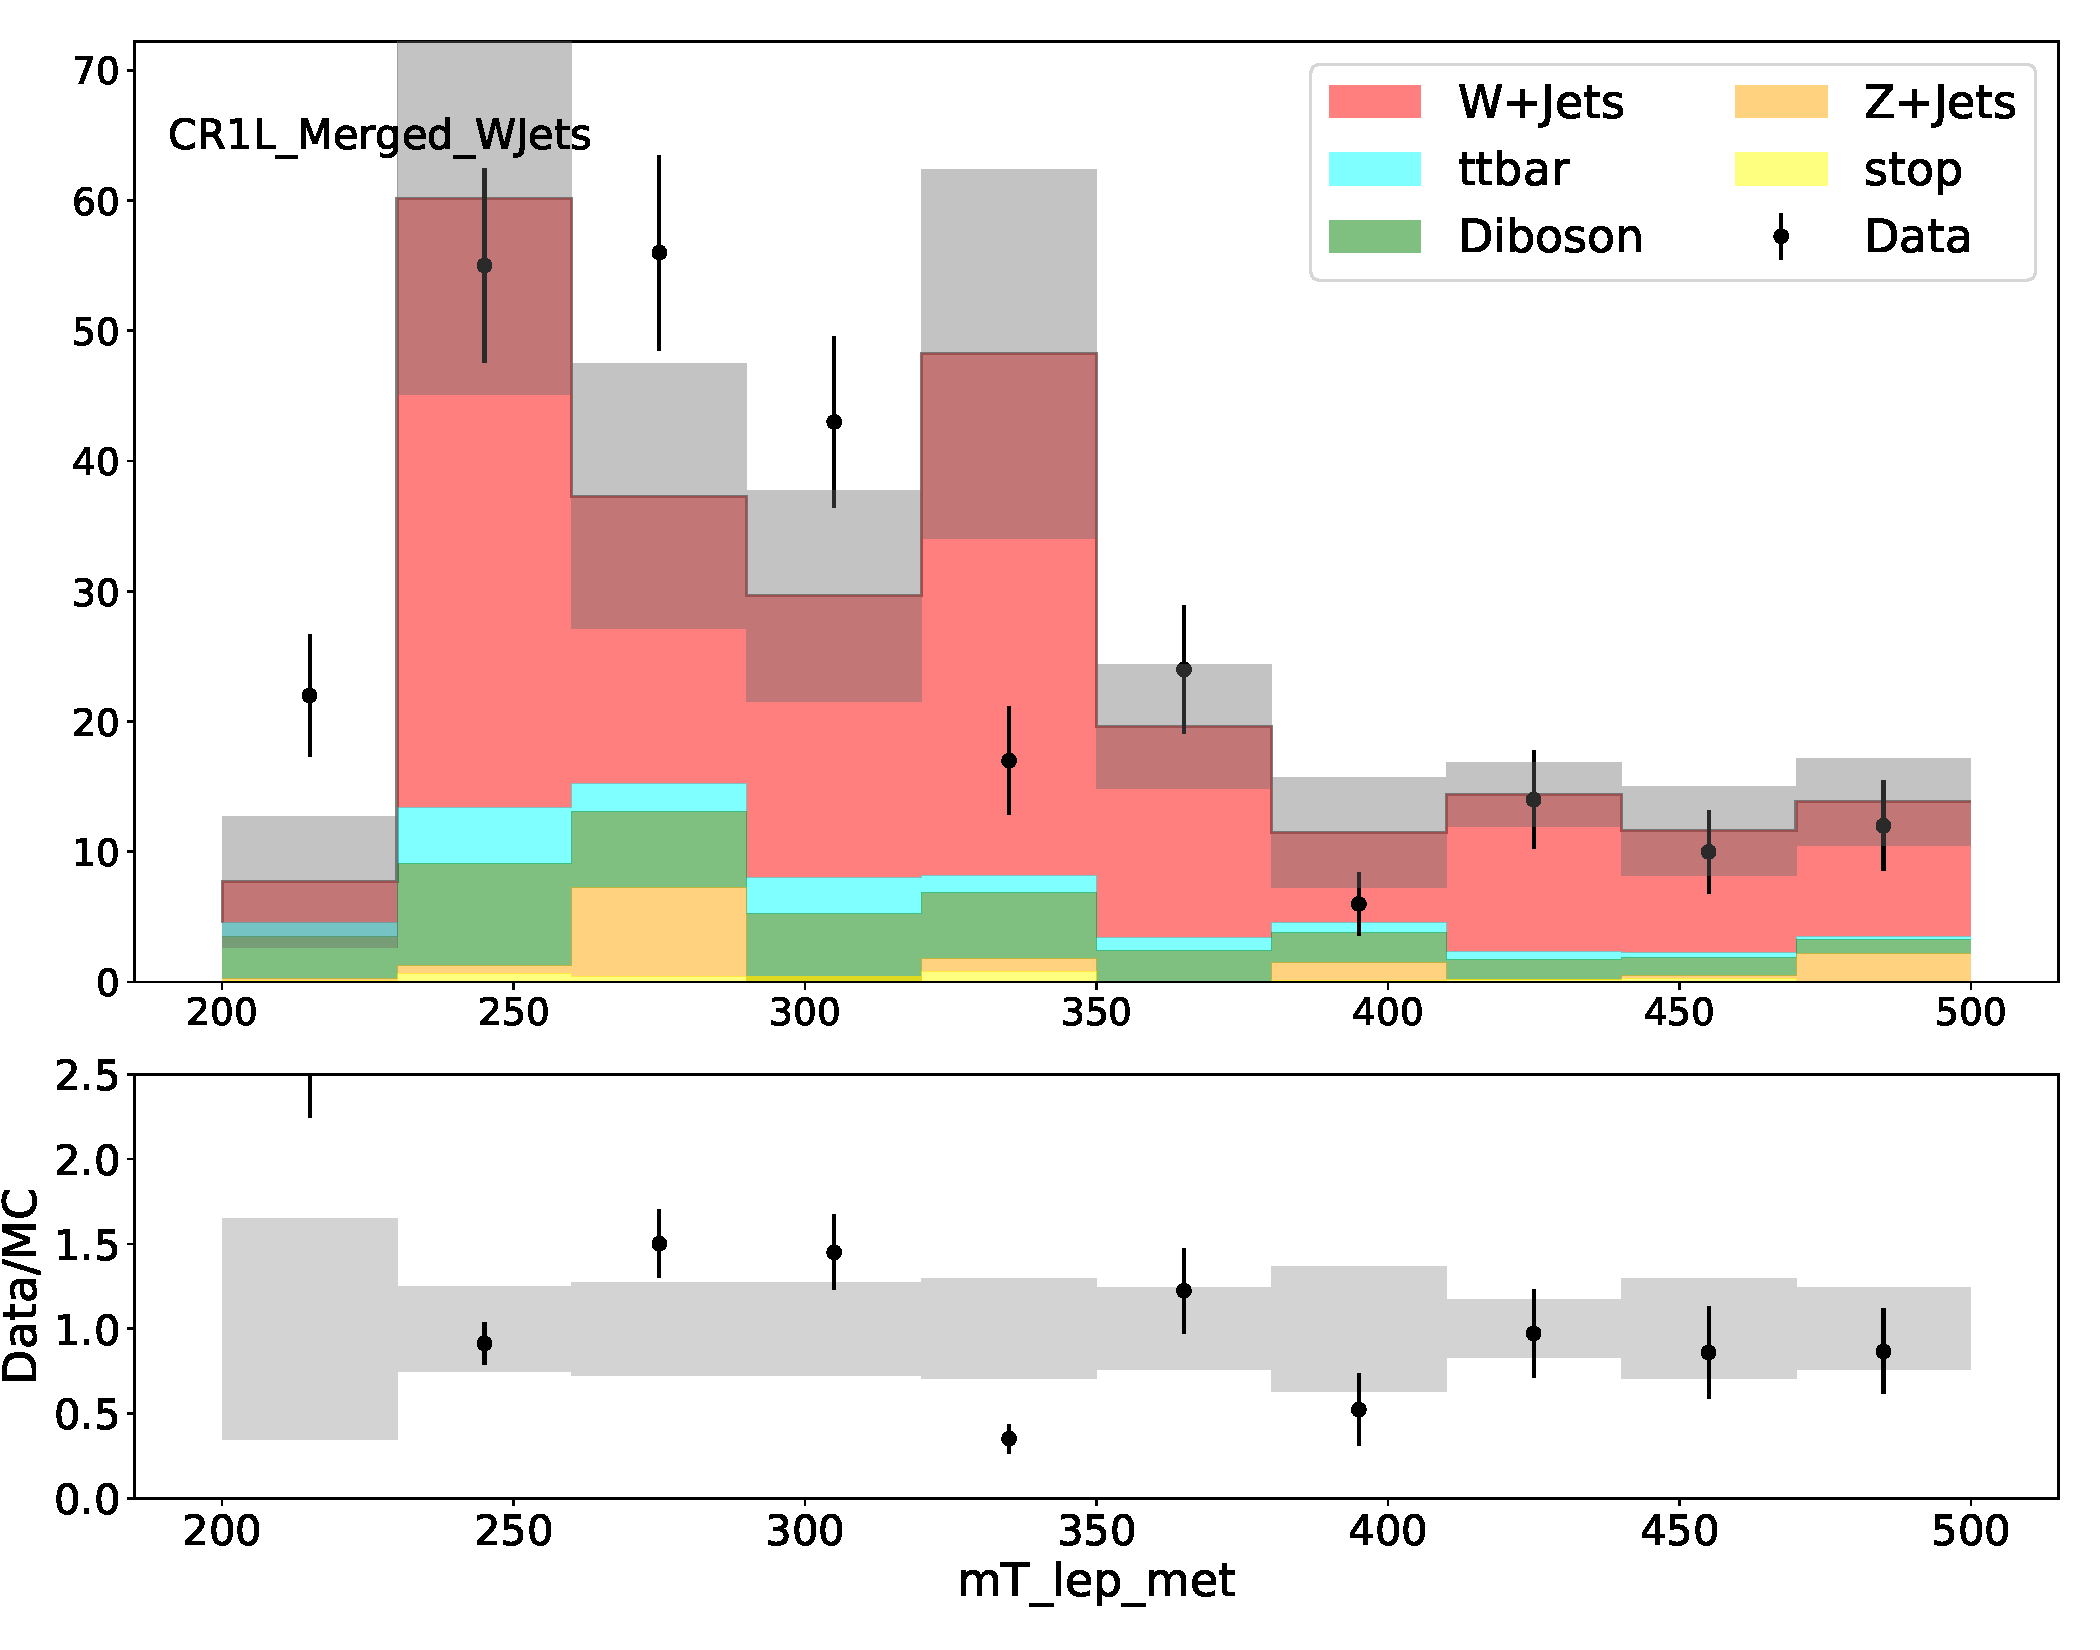
\includegraphics[width = 0.98\textwidth]{Figures/4/datamc/CR1L_Merged_WJets/mT_lep_met.pdf}
    \caption{\mtlepmet}
     \end{subfigure}
    \begin{subfigure}{0.49\textwidth}
     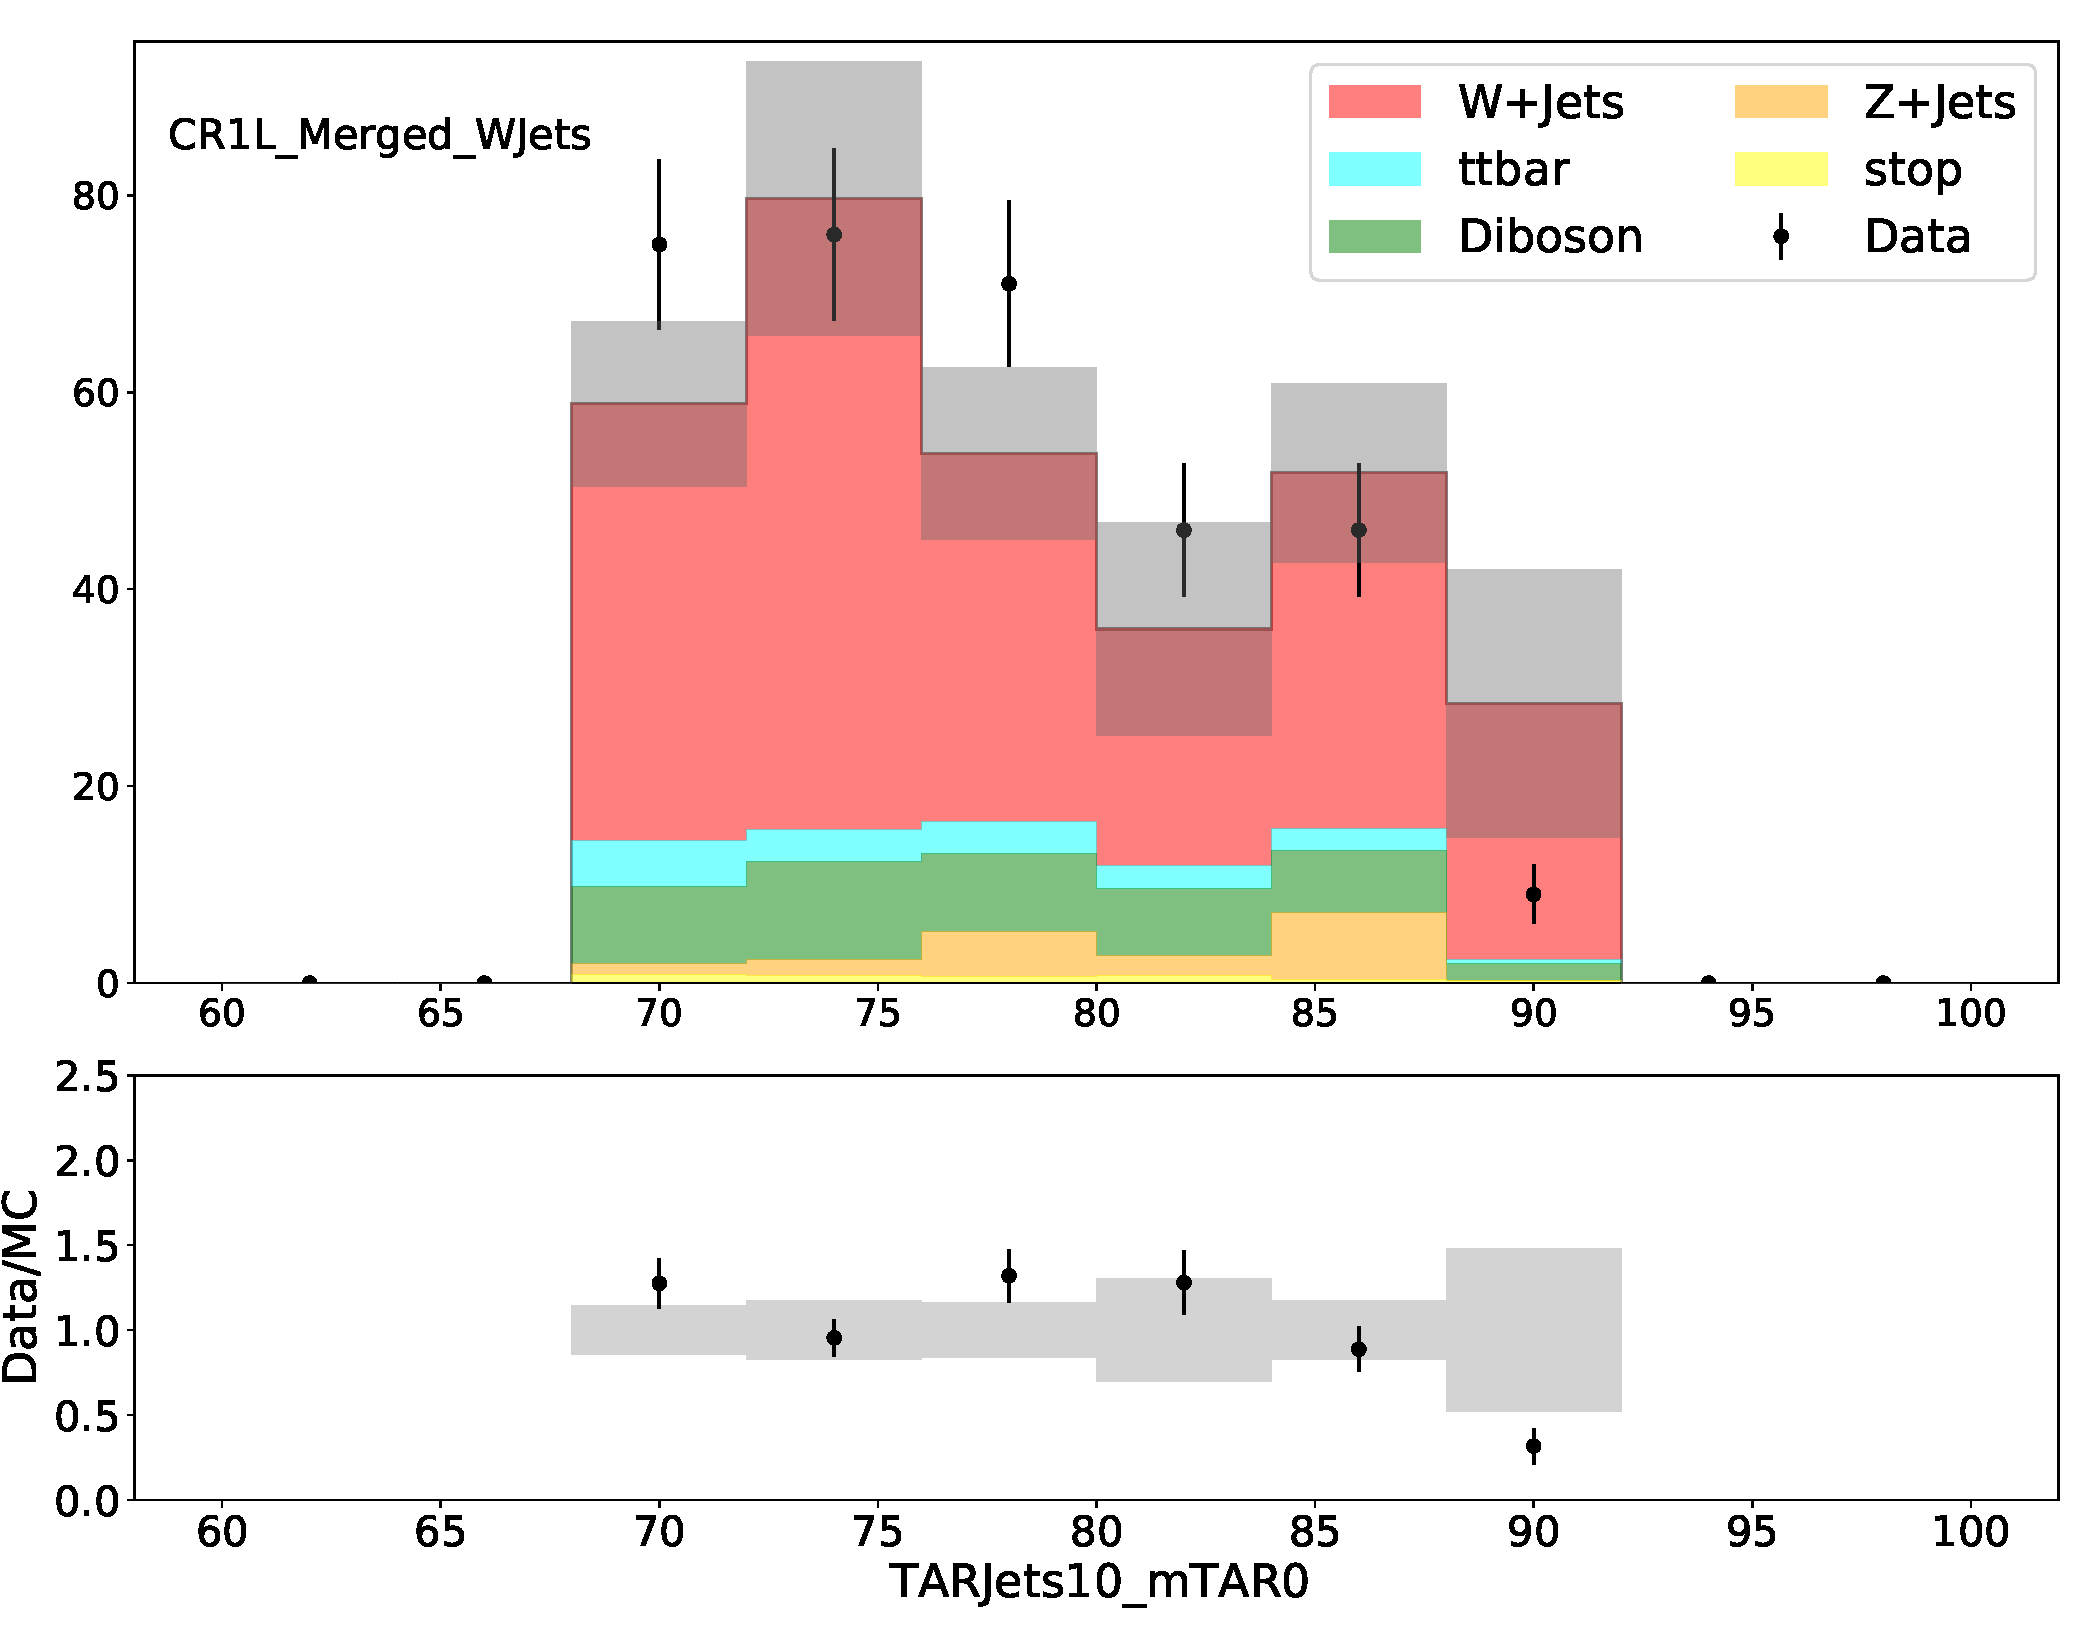
\includegraphics[width = 0.98\textwidth]{Figures/4/datamc/CR1L_Merged_WJets/TARJets10_mTAR0.pdf}
     \caption{\mTAR}
     \end{subfigure}
    \begin{subfigure}{0.49\textwidth}
     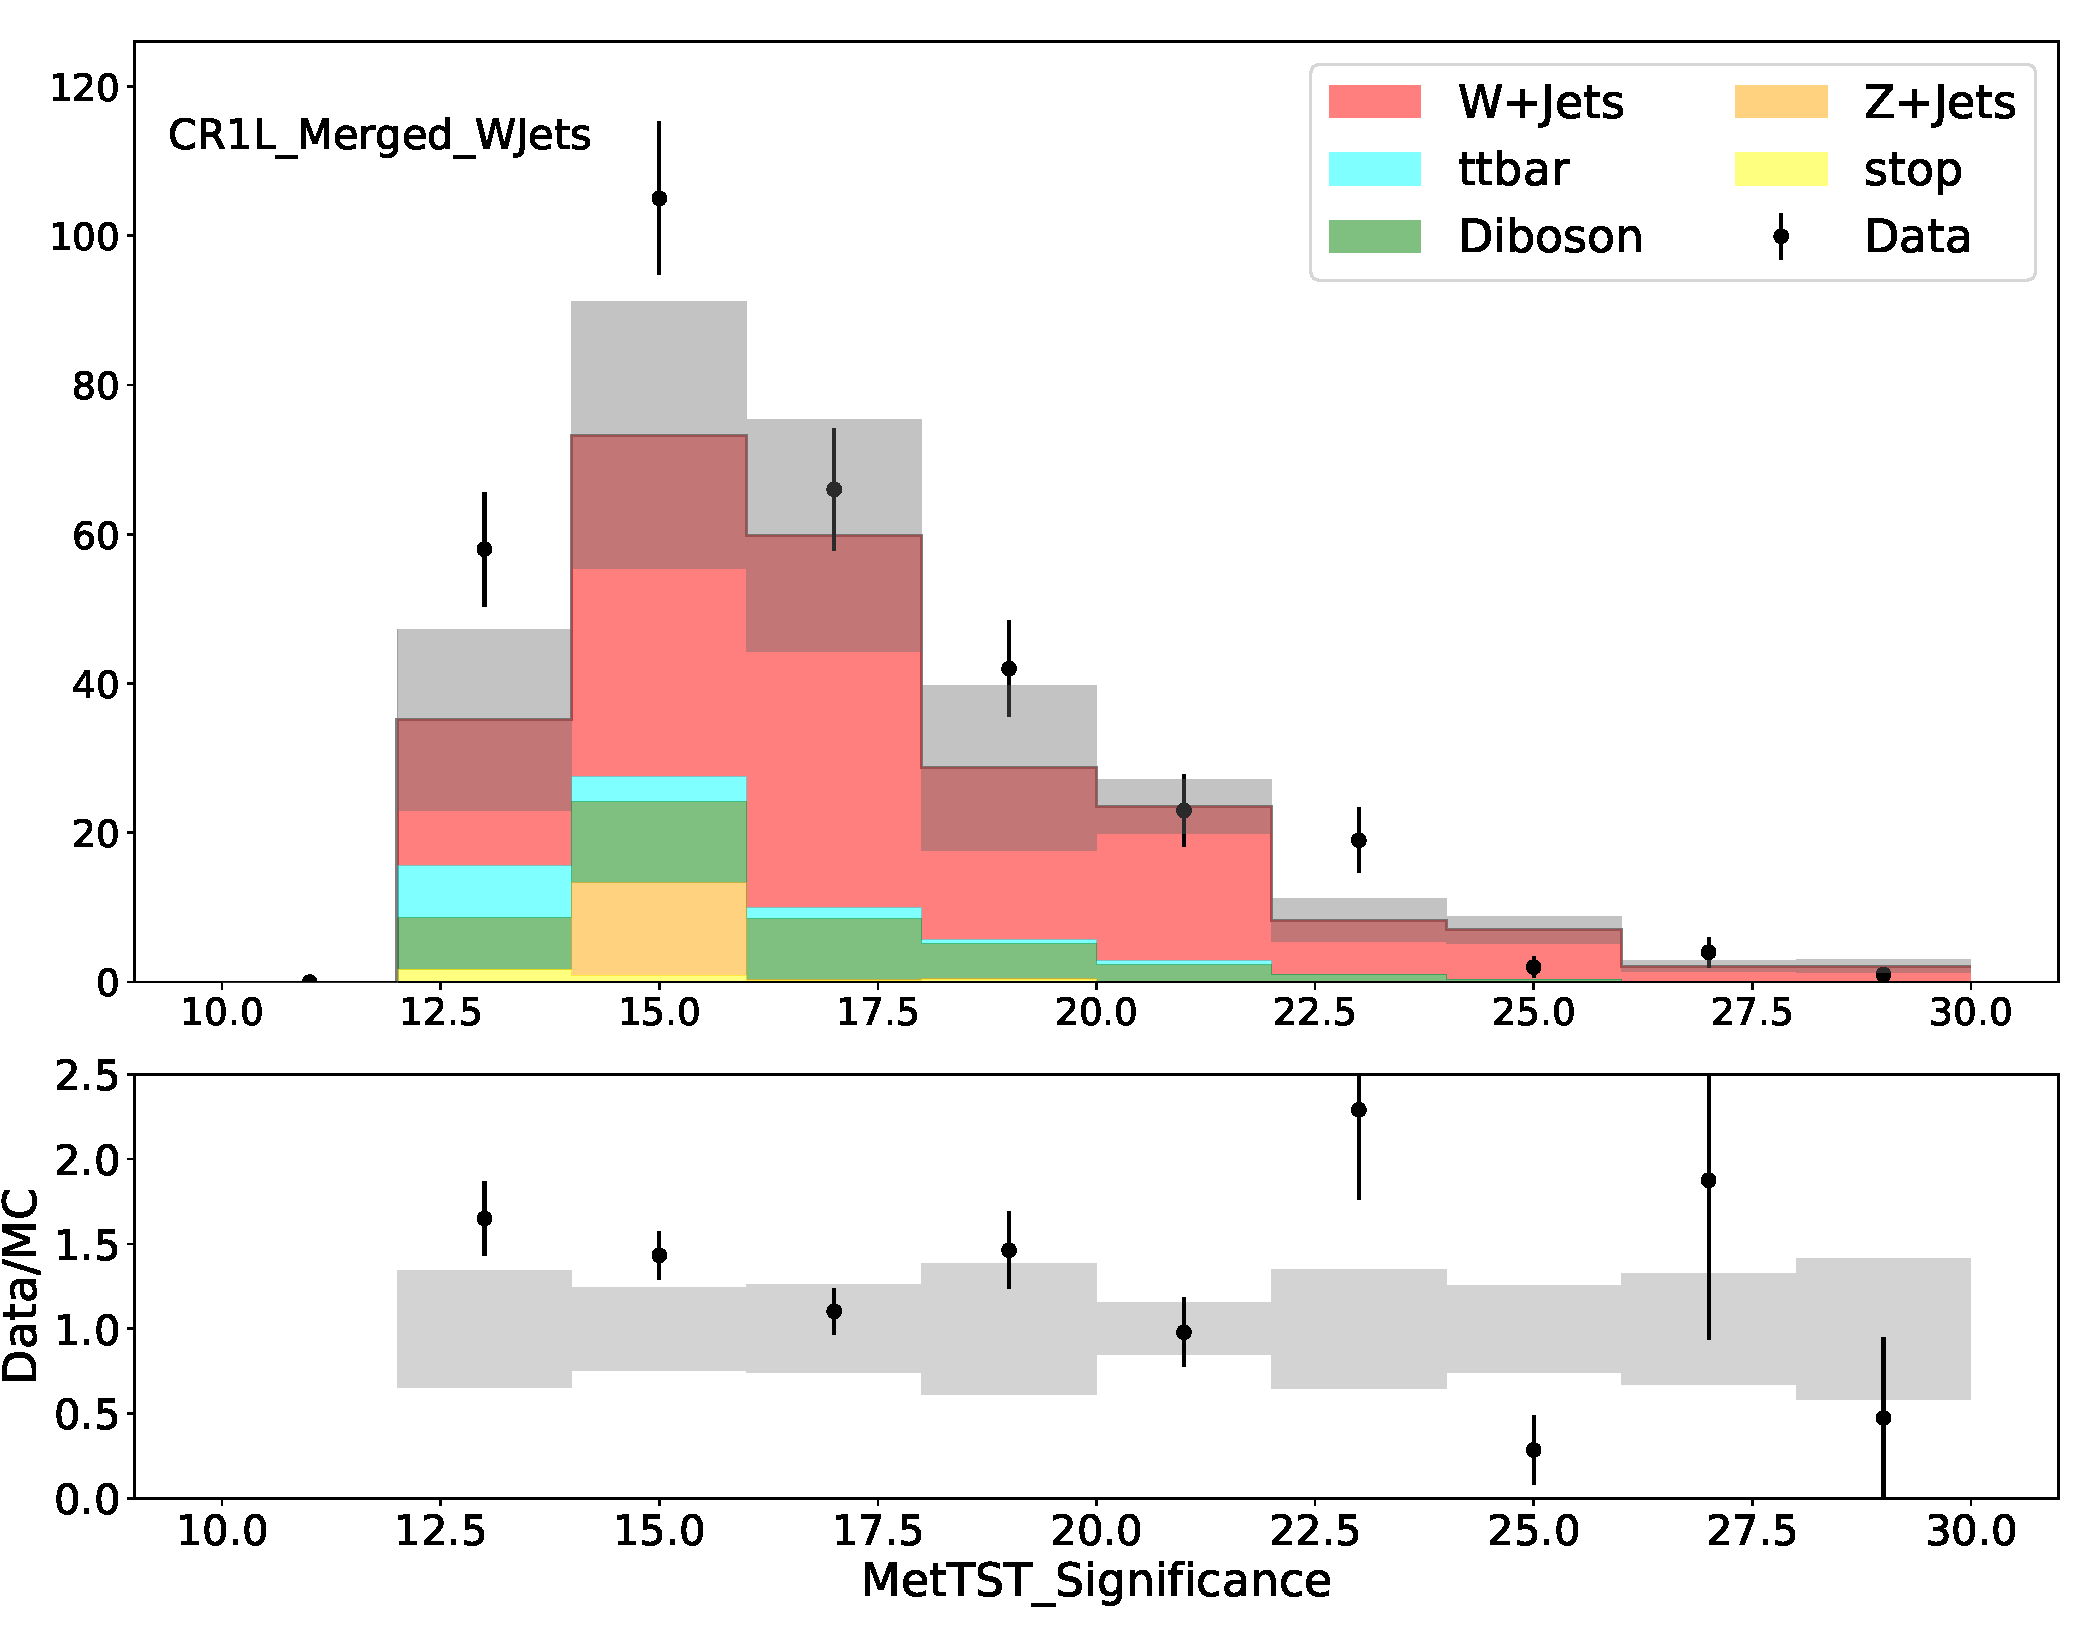
\includegraphics[width = 0.98\textwidth]{Figures/4/datamc/CR1L_Merged_WJets/MetTST_Significance.pdf}
     \caption{\metsig}
     \end{subfigure}
    \begin{subfigure}{0.49\textwidth}
     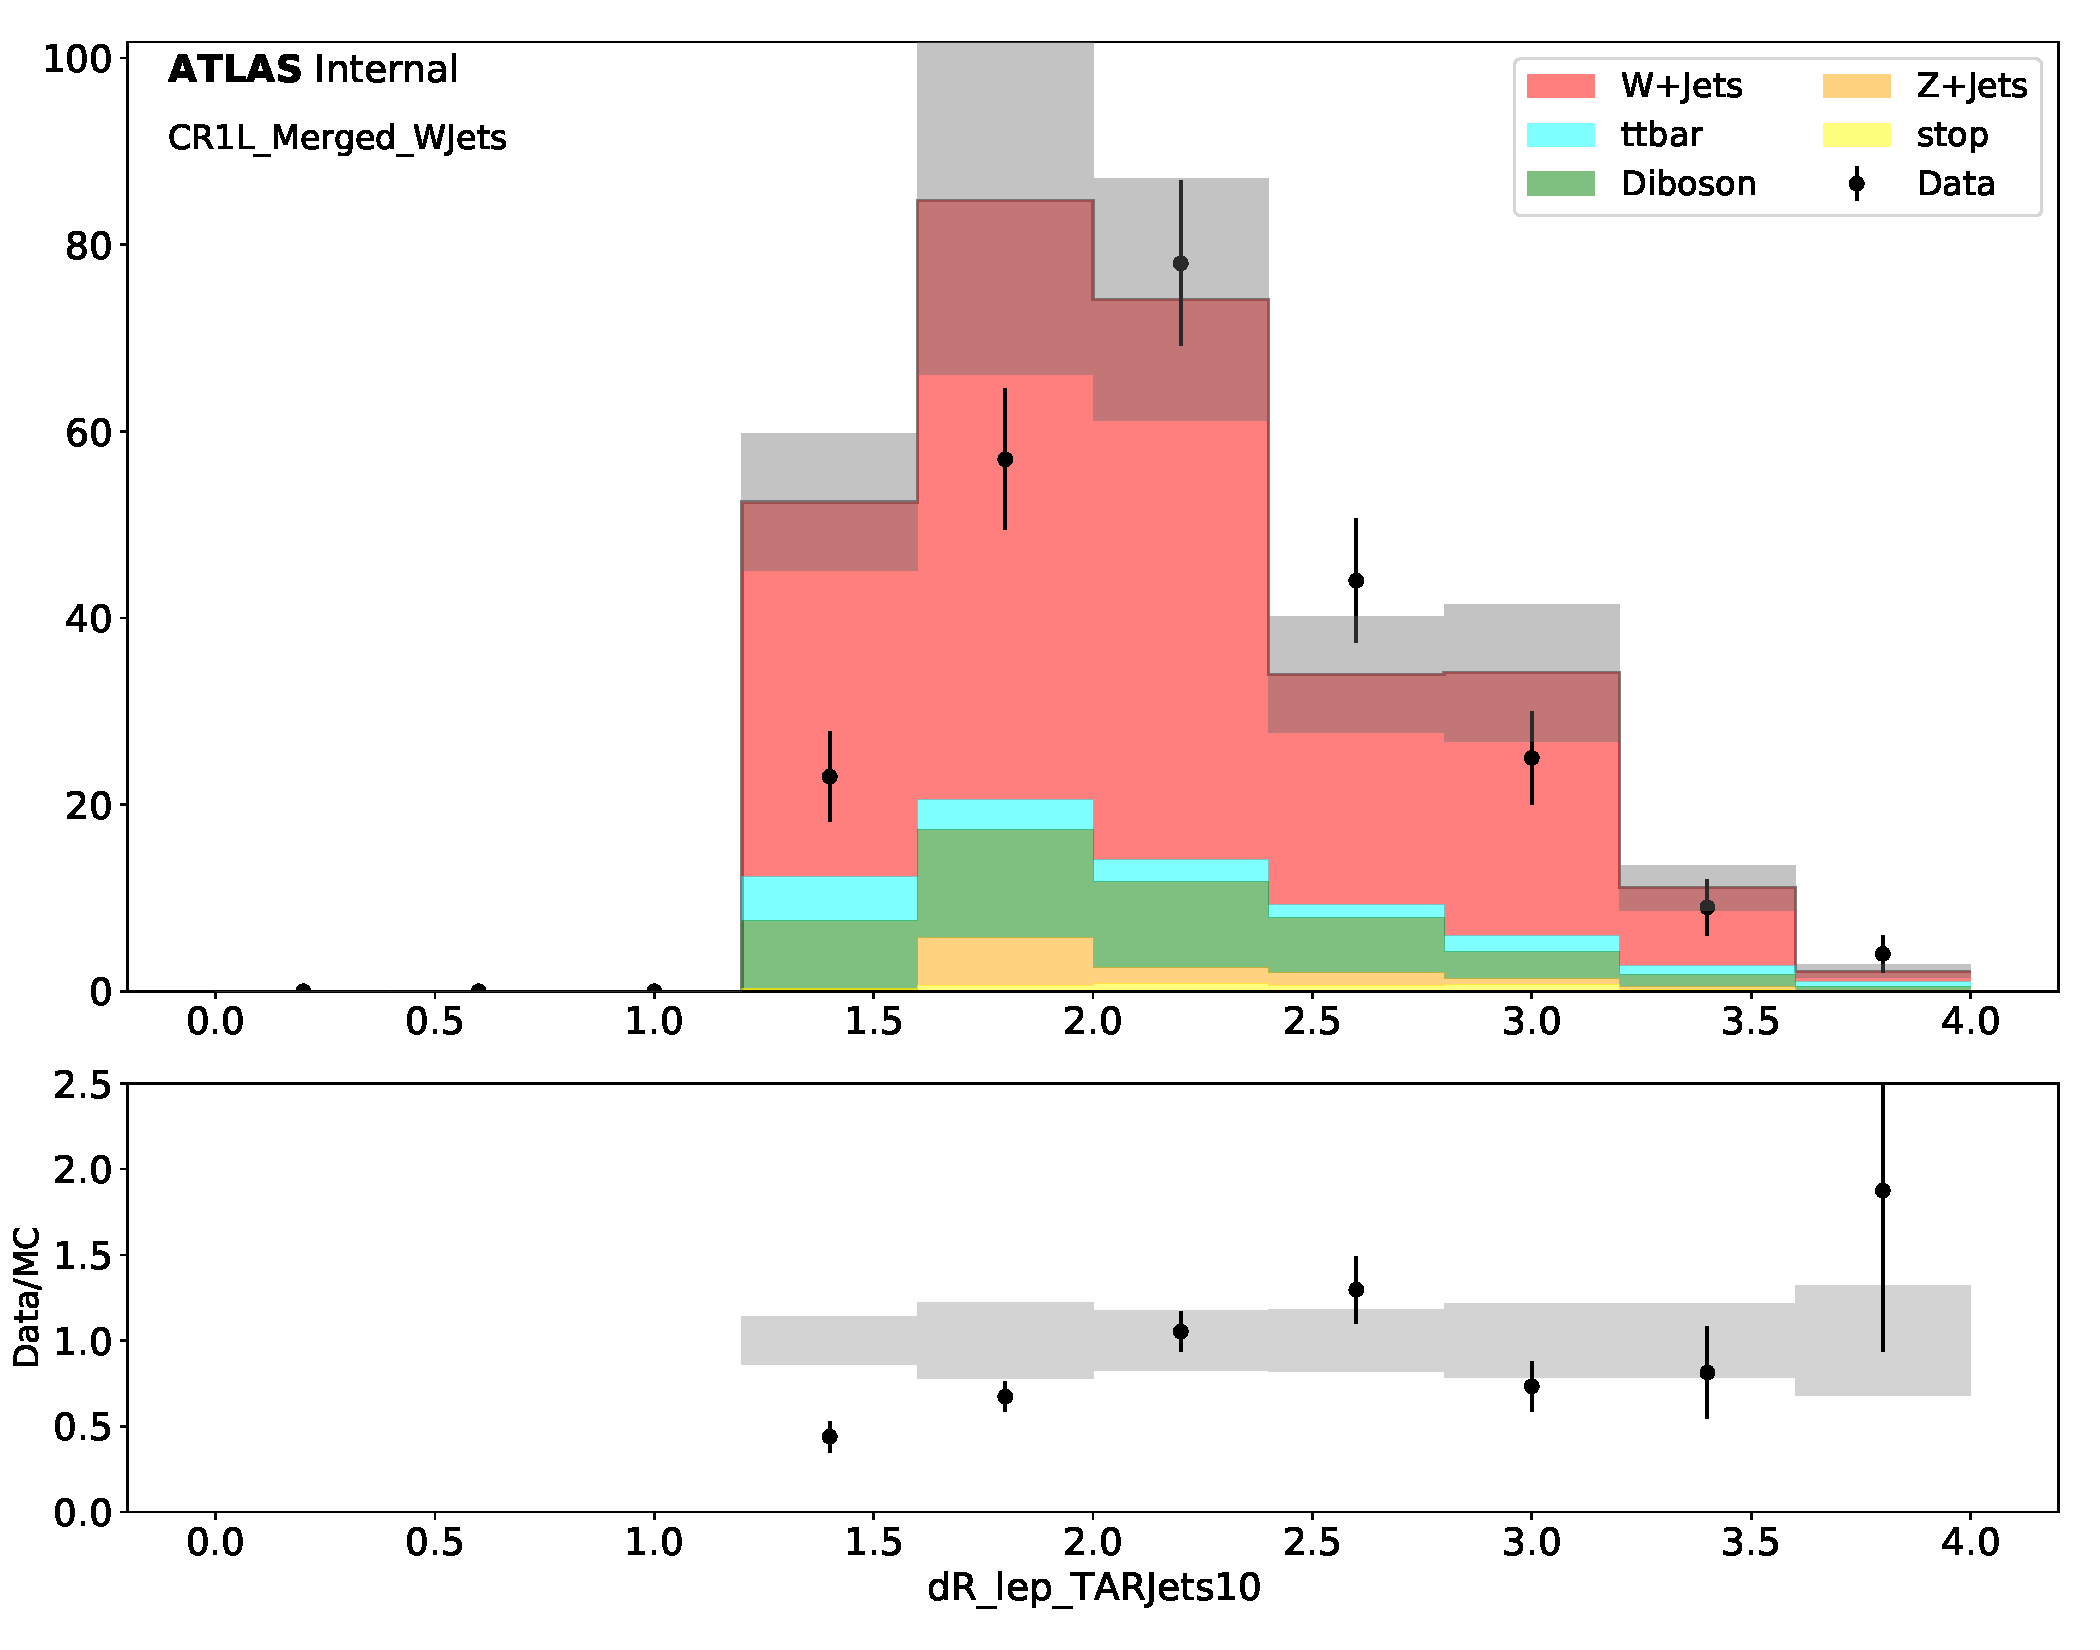
\includegraphics[width = 0.98\textwidth]{Figures/4/datamc/CR1L_Merged_WJets/dR_lep_TARJets10.pdf}
     \caption{\drTARl}
     \end{subfigure}
     \begin{subfigure}{0.49\textwidth}
     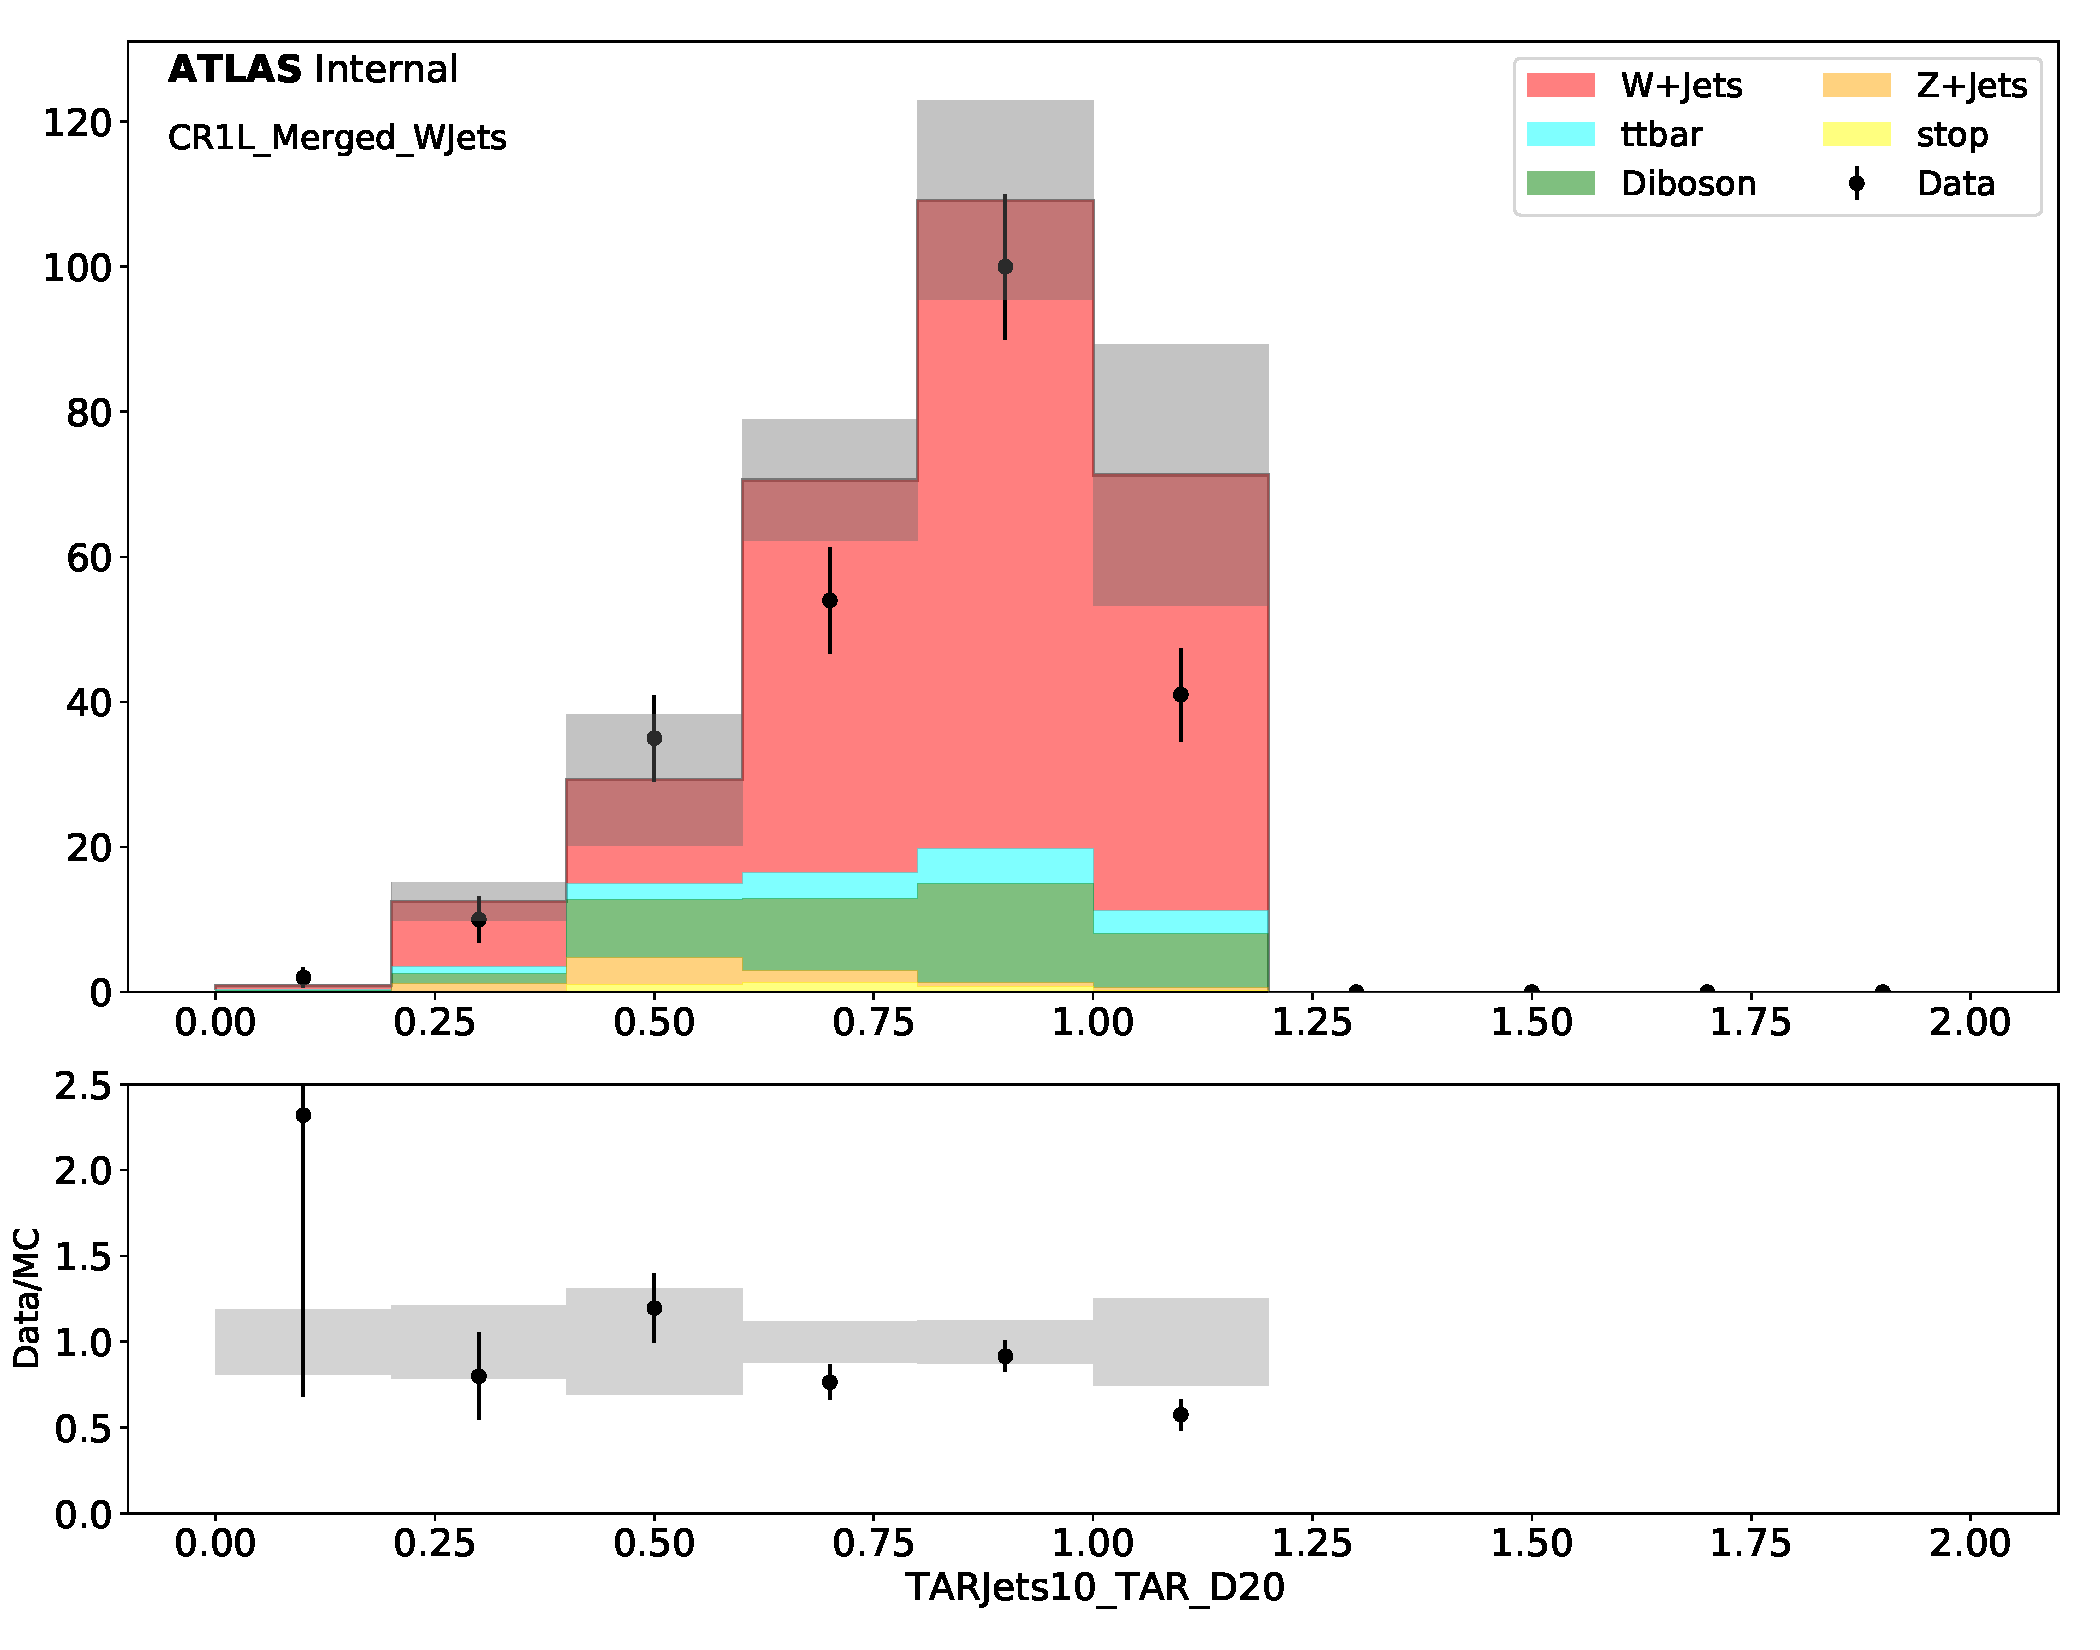
\includegraphics[width = 0.98\textwidth]{Figures/4/datamc/CR1L_Merged_WJets/TARJets10_TAR_D20.pdf}
     \caption{\DtwoTAR}
     \end{subfigure}
     \begin{subfigure}{0.49\textwidth}
     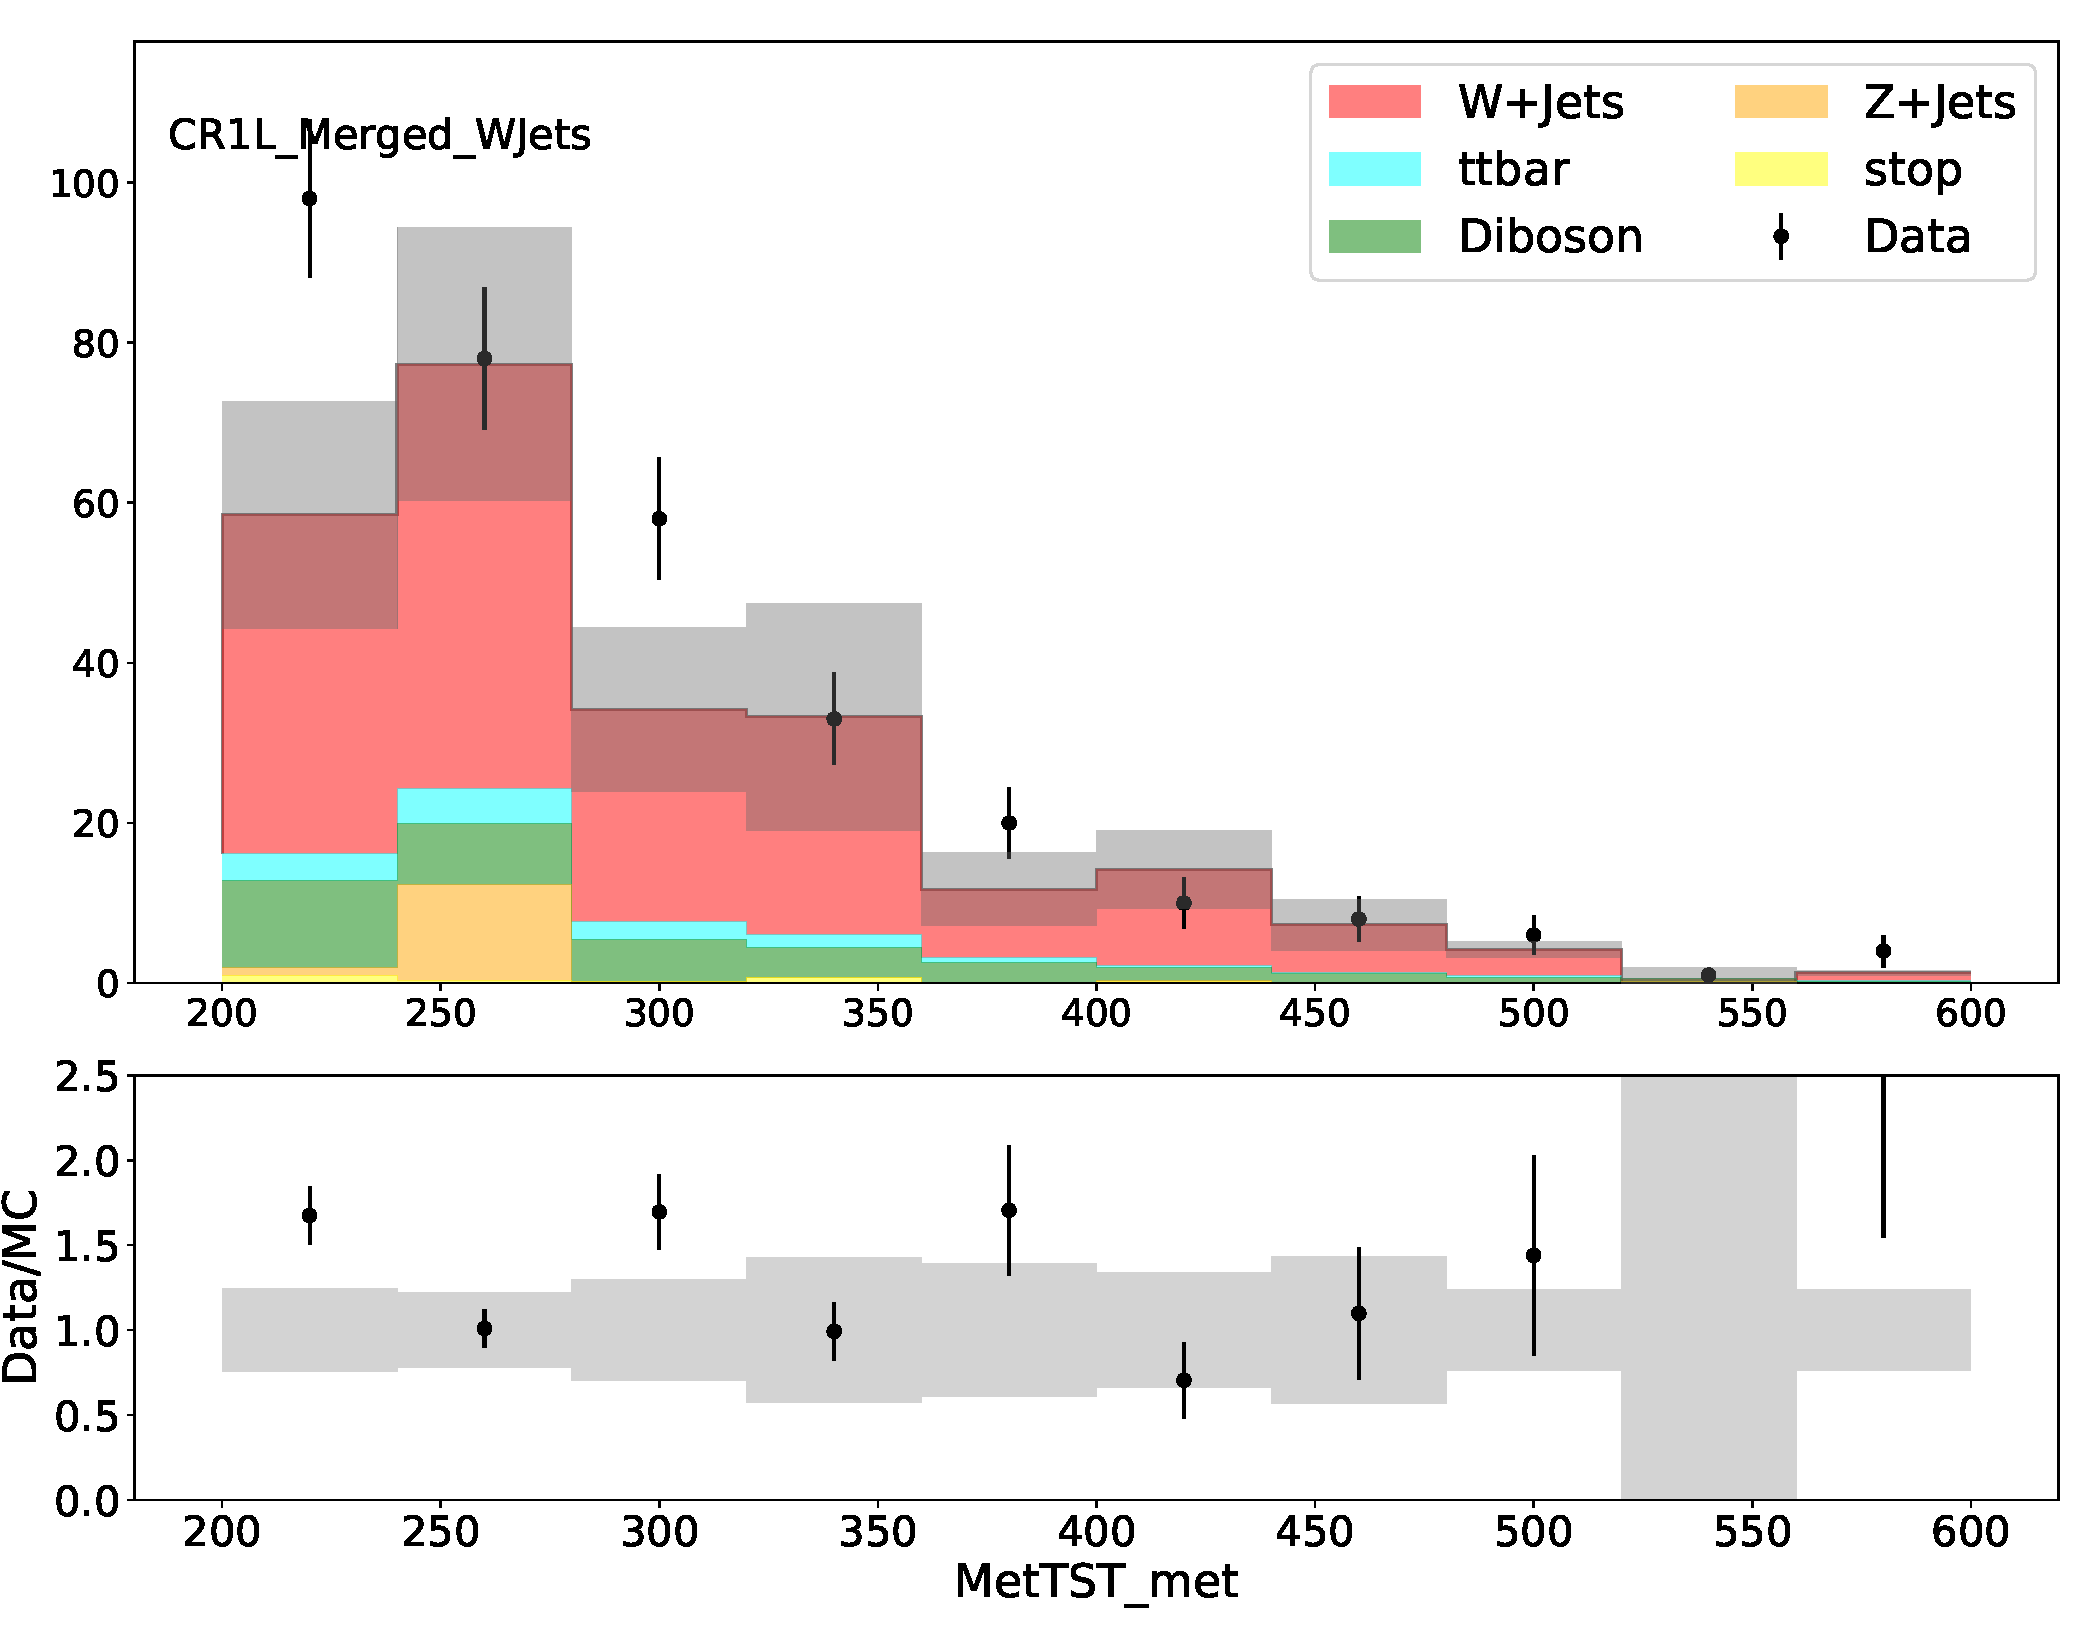
\includegraphics[width = 0.98\textwidth]{Figures/4/datamc/CR1L_Merged_WJets/MetTST_met.pdf}
     \caption{\met}
     \end{subfigure}

     \caption{Data-MC comparisons in the \merged \wjets control region}
     \label{fig:Data_MC_CRdR_merged}
  \end{figure}

\begin{figure}[htbp]
  \centering
     \begin{subfigure}{0.49\textwidth}
     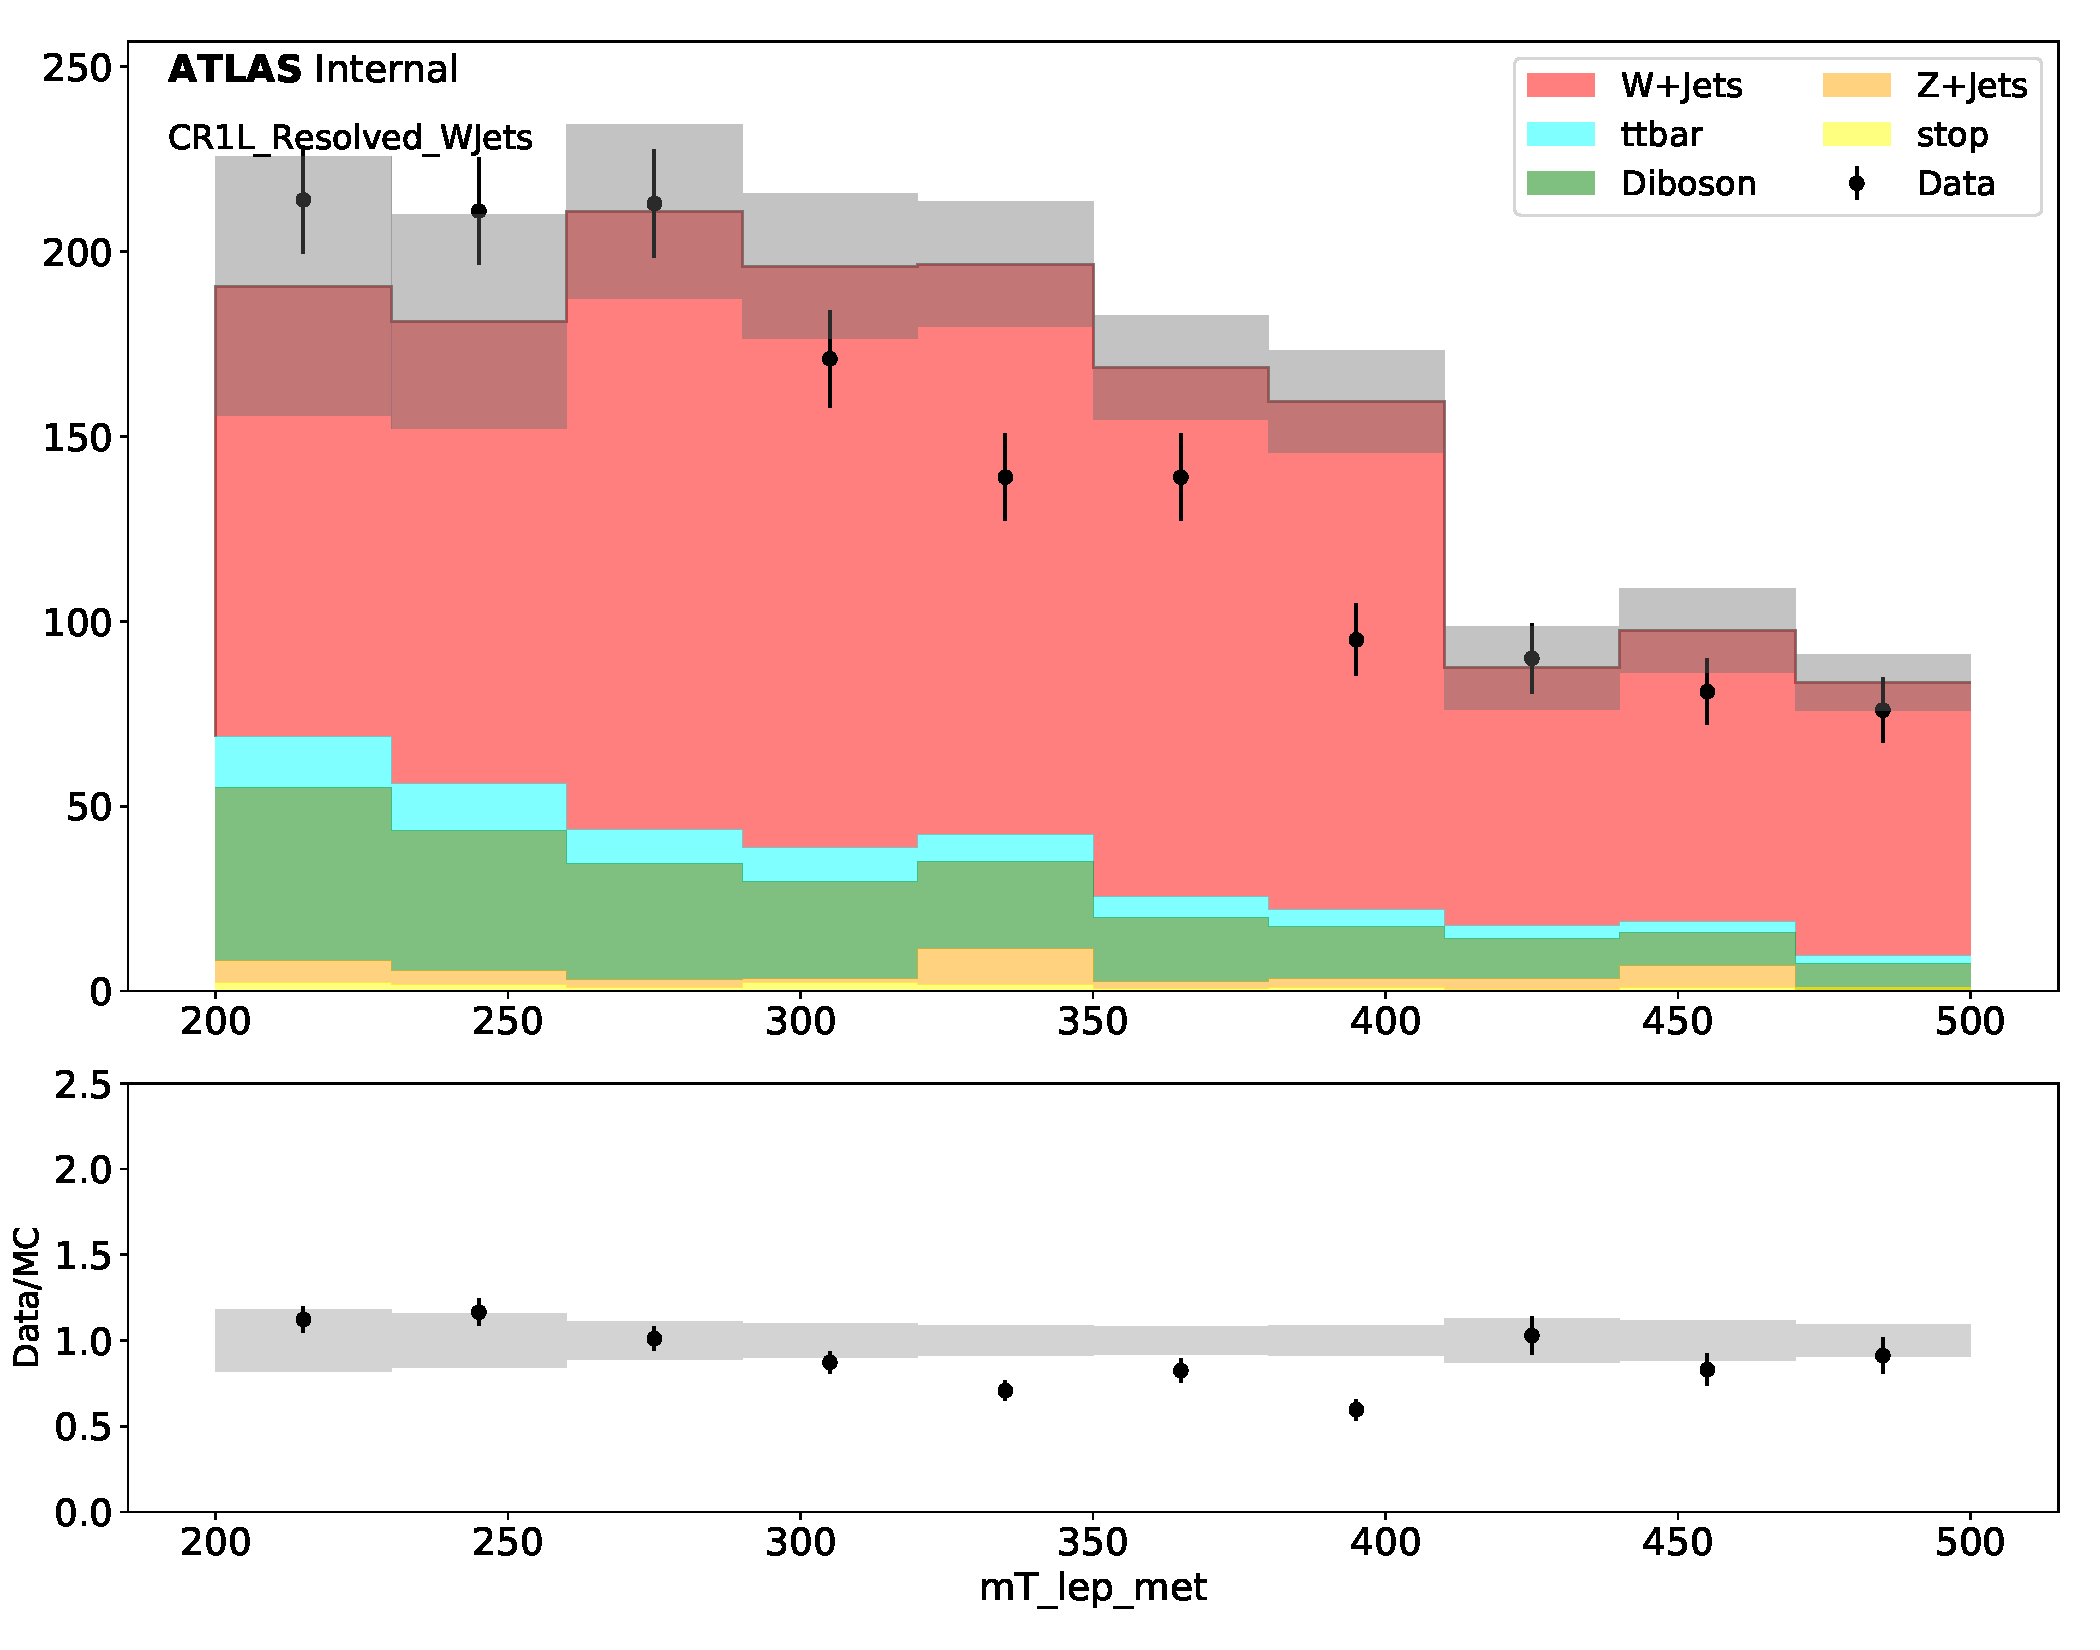
\includegraphics[width = 0.98\textwidth]{Figures/4/datamc/CR1L_Resolved_WJets/mT_lep_met.pdf}
     \caption{\mtlepmet}
     \end{subfigure}
     \begin{subfigure}{0.49\textwidth}
     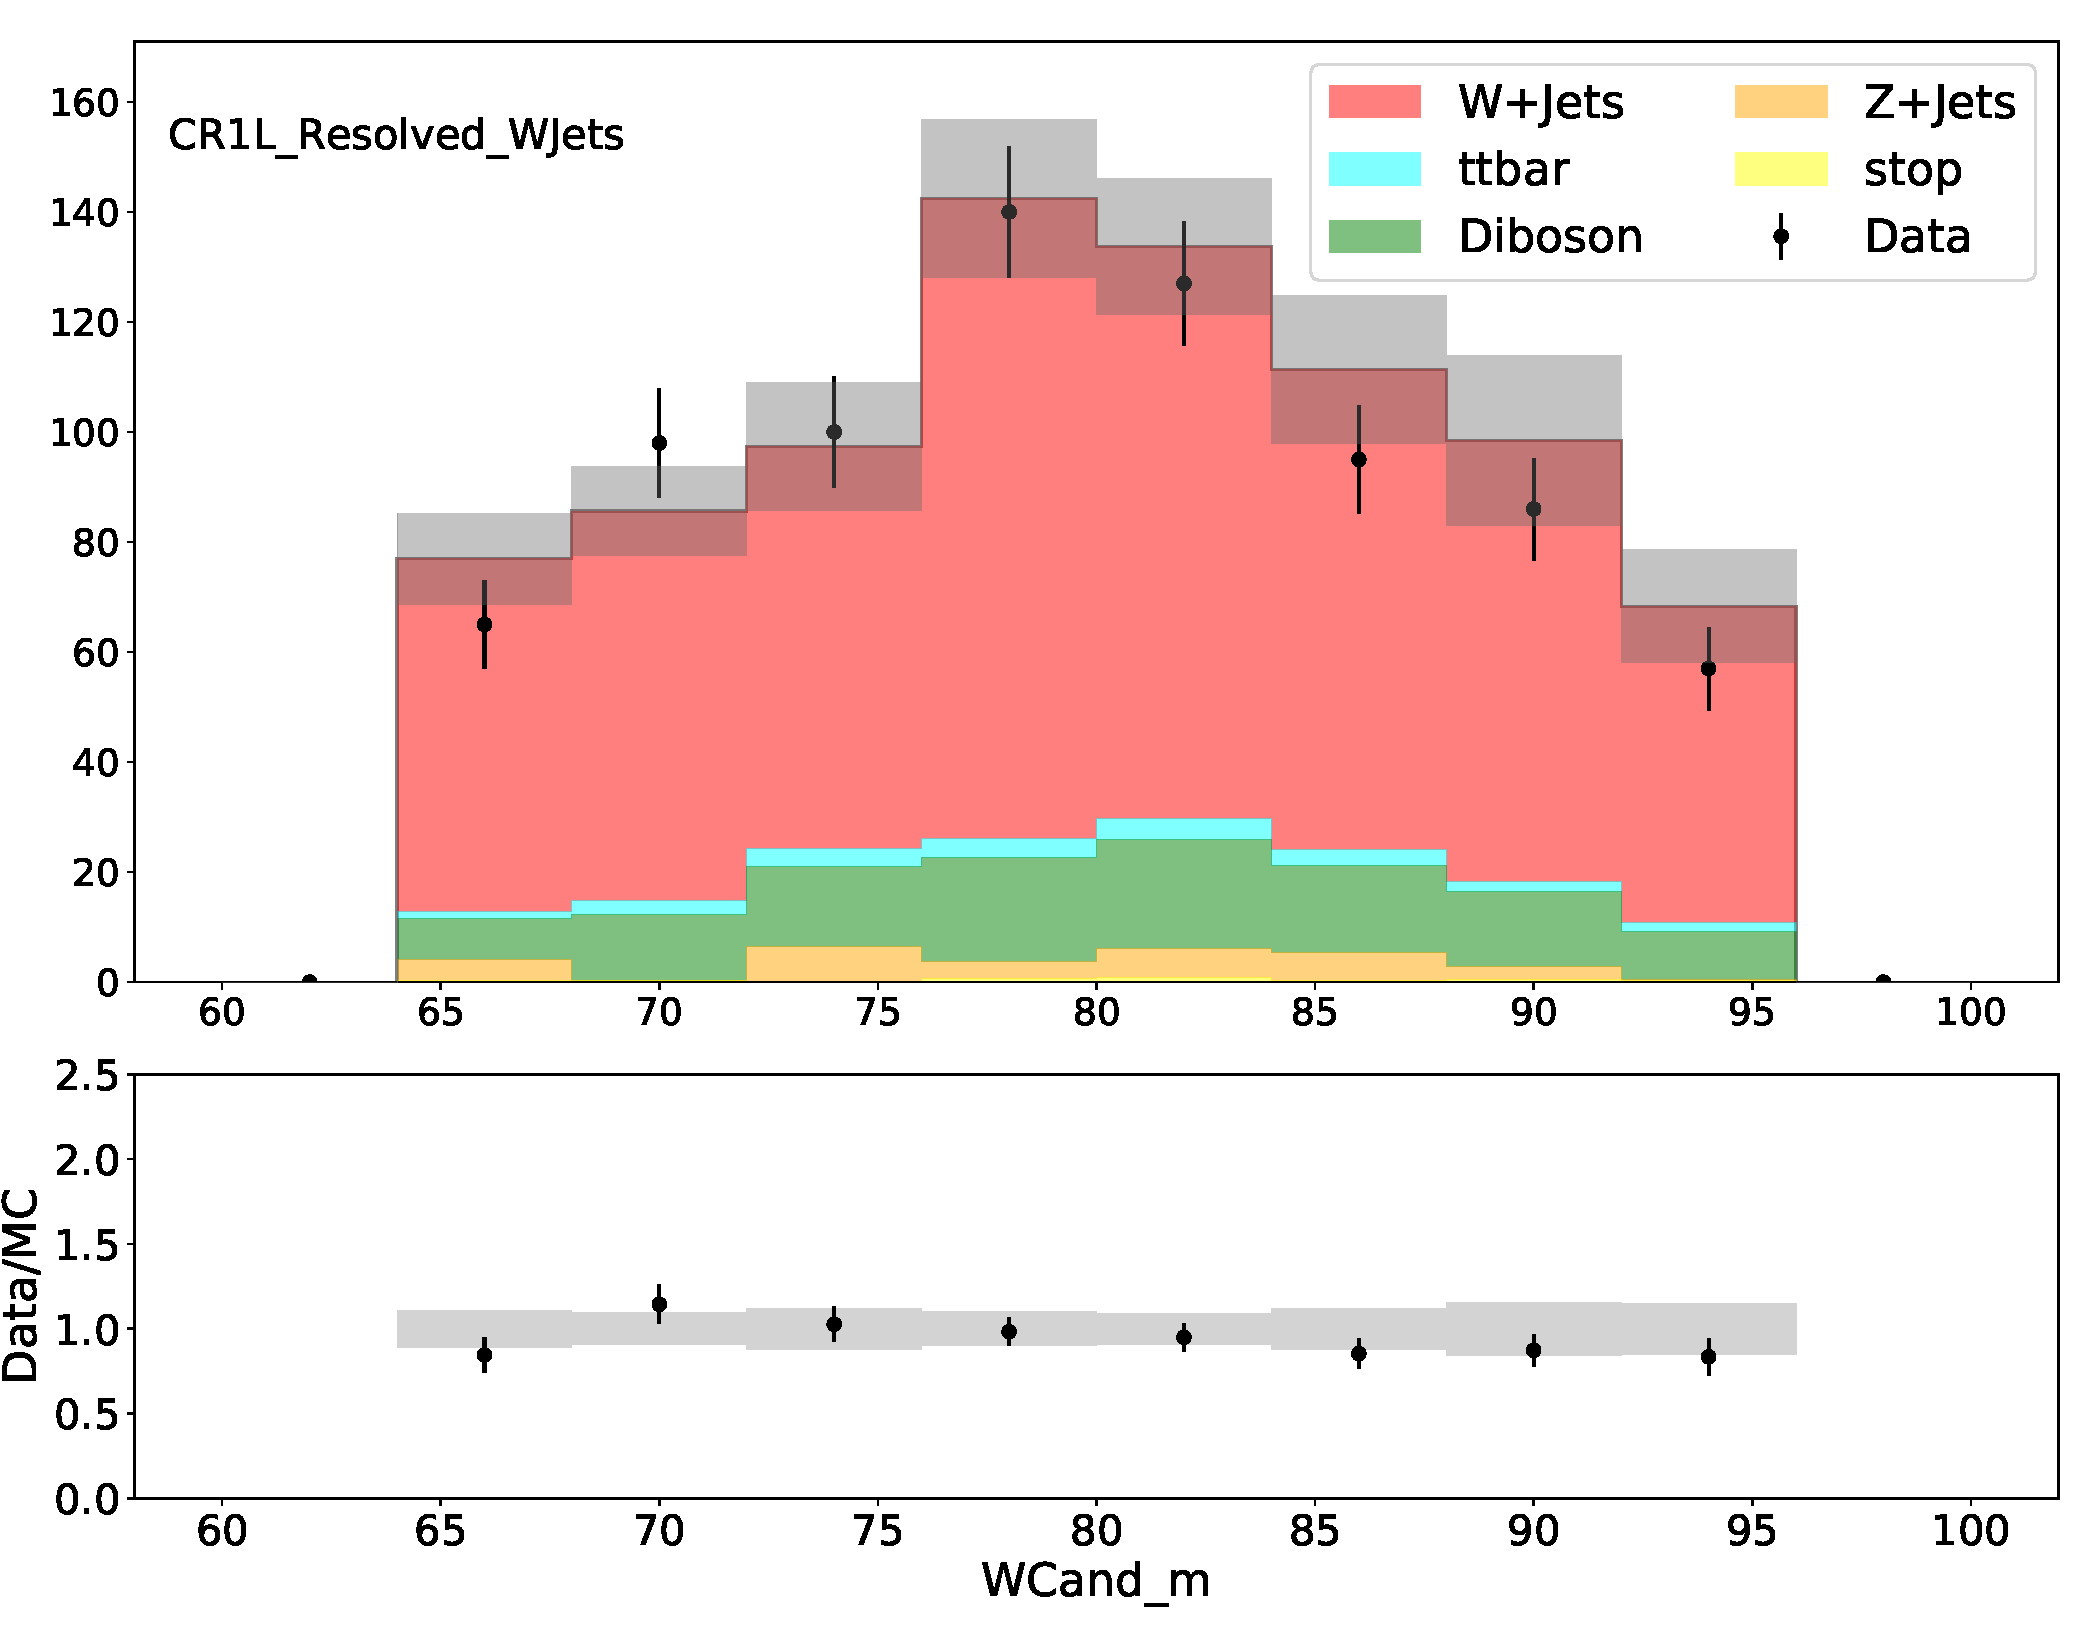
\includegraphics[width = 0.98\textwidth]{Figures/4/datamc/CR1L_Resolved_WJets/WCand_m.pdf}
     \caption{\Wcandm}
     \end{subfigure}
     \begin{subfigure}{0.49\textwidth}
     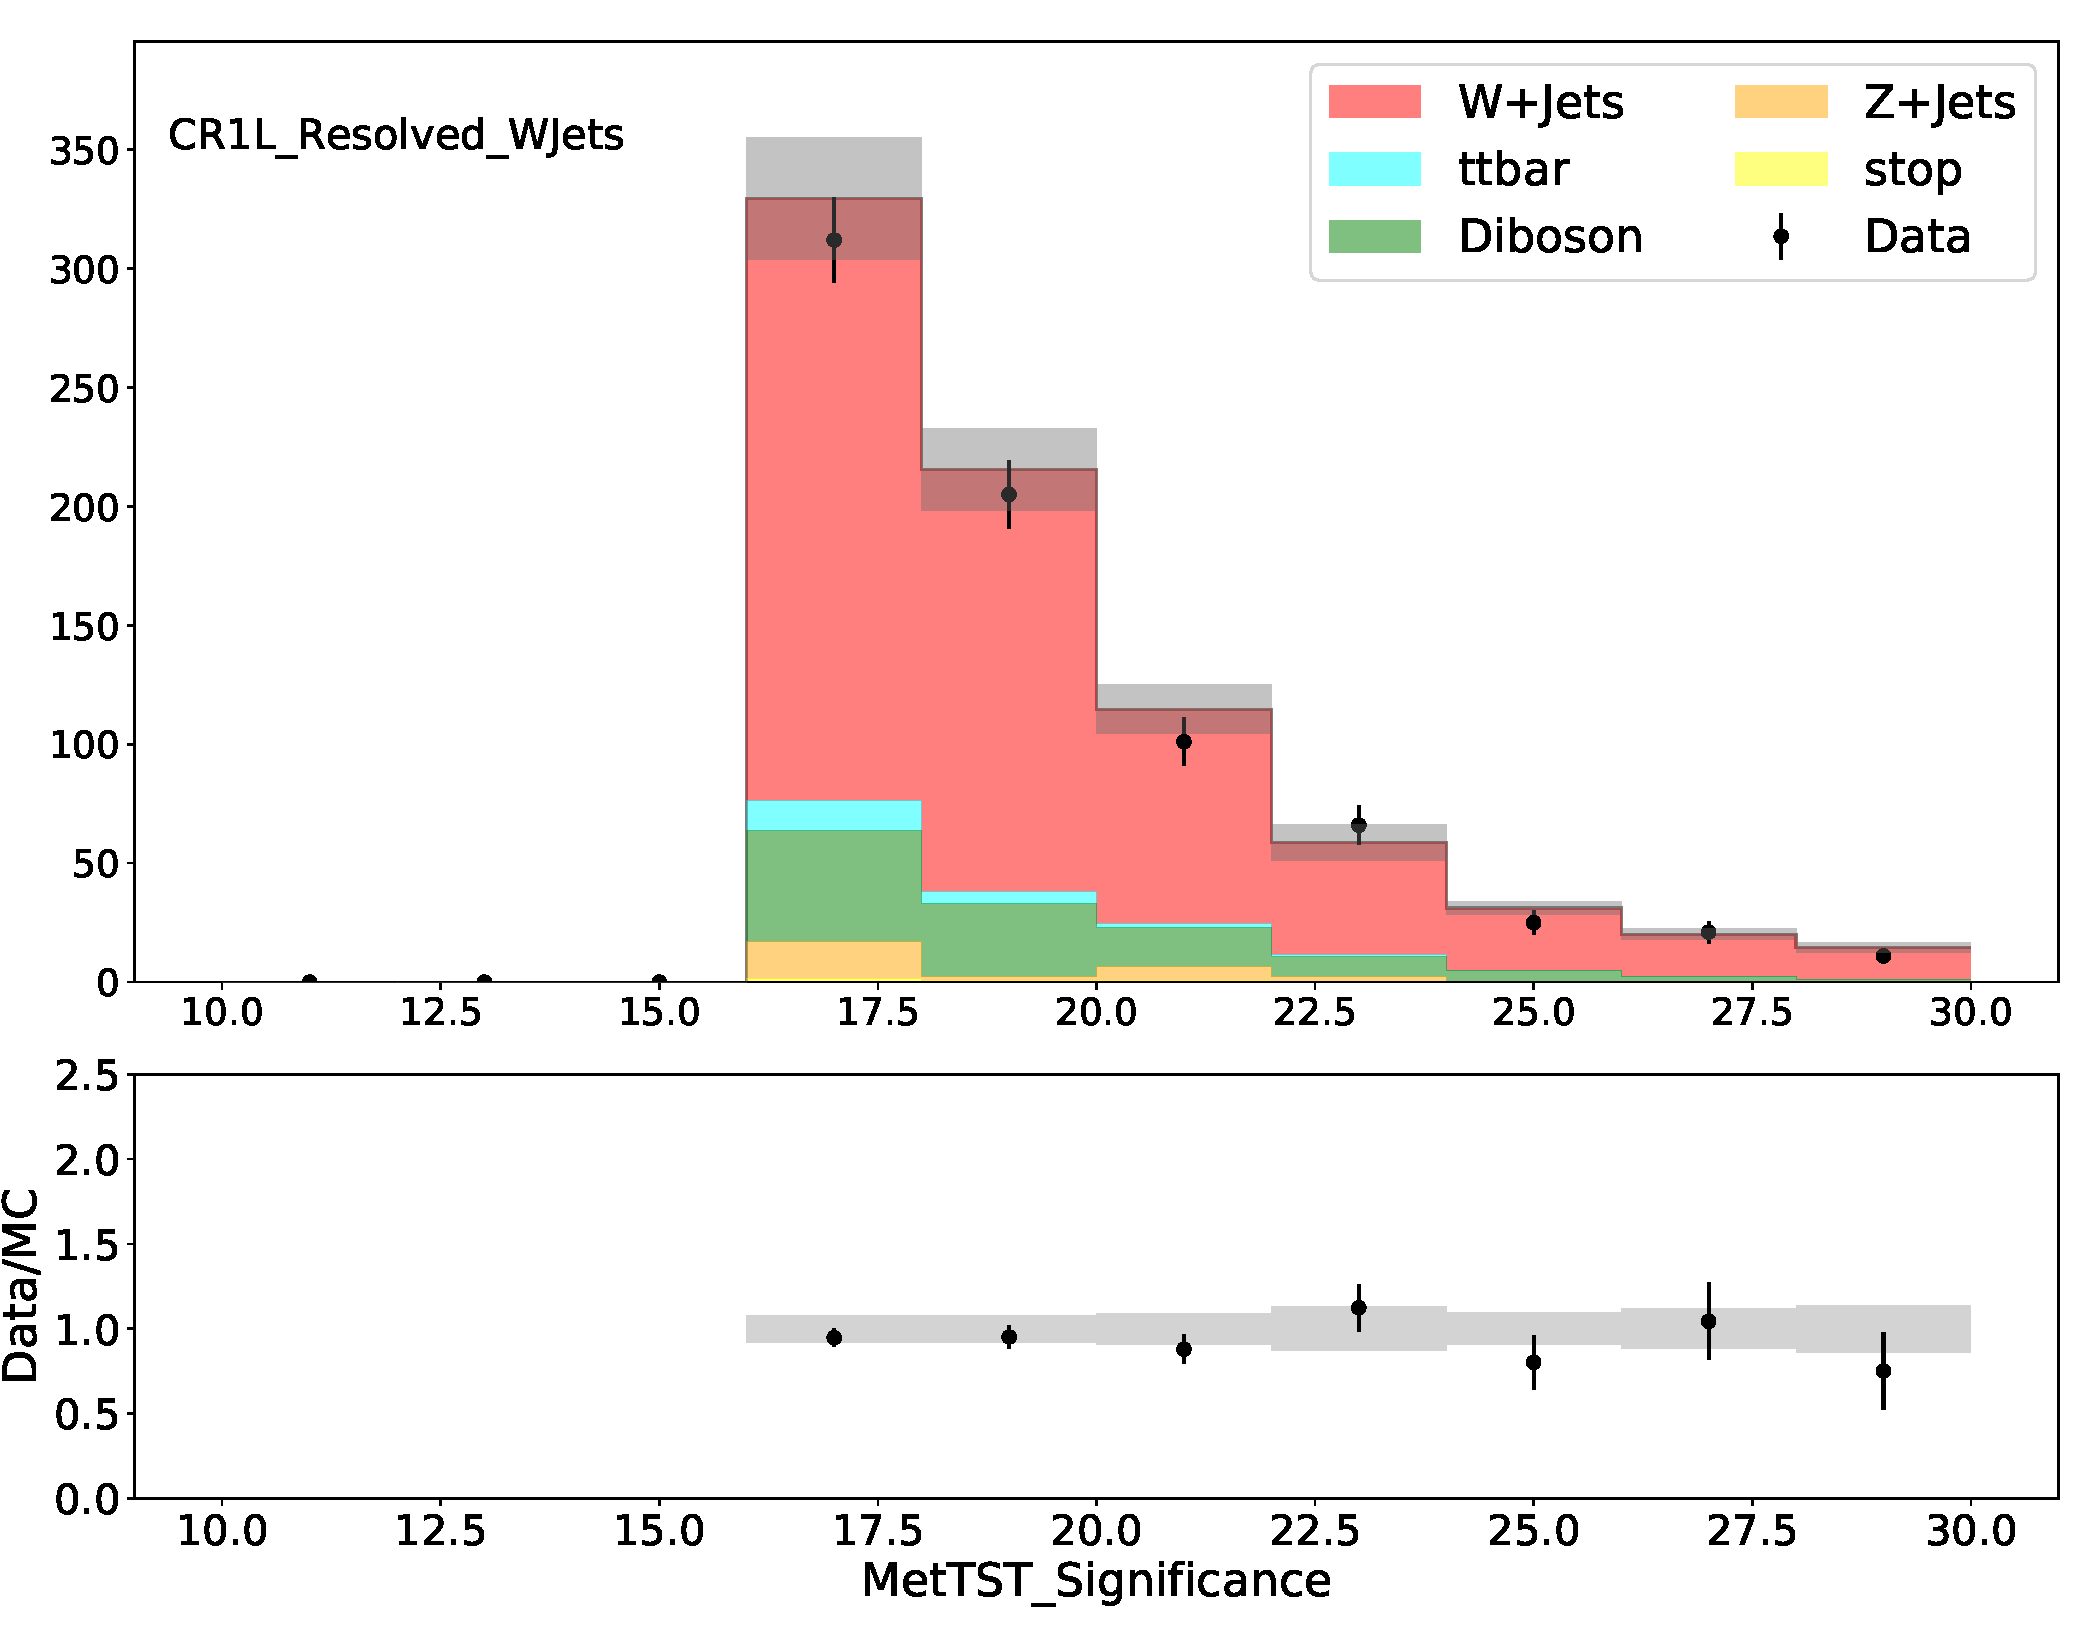
\includegraphics[width = 0.98\textwidth]{Figures/4/datamc/CR1L_Resolved_WJets/MetTST_Significance.pdf}
     \caption{\metsig}
     \end{subfigure}
     \begin{subfigure}{0.49\textwidth}
     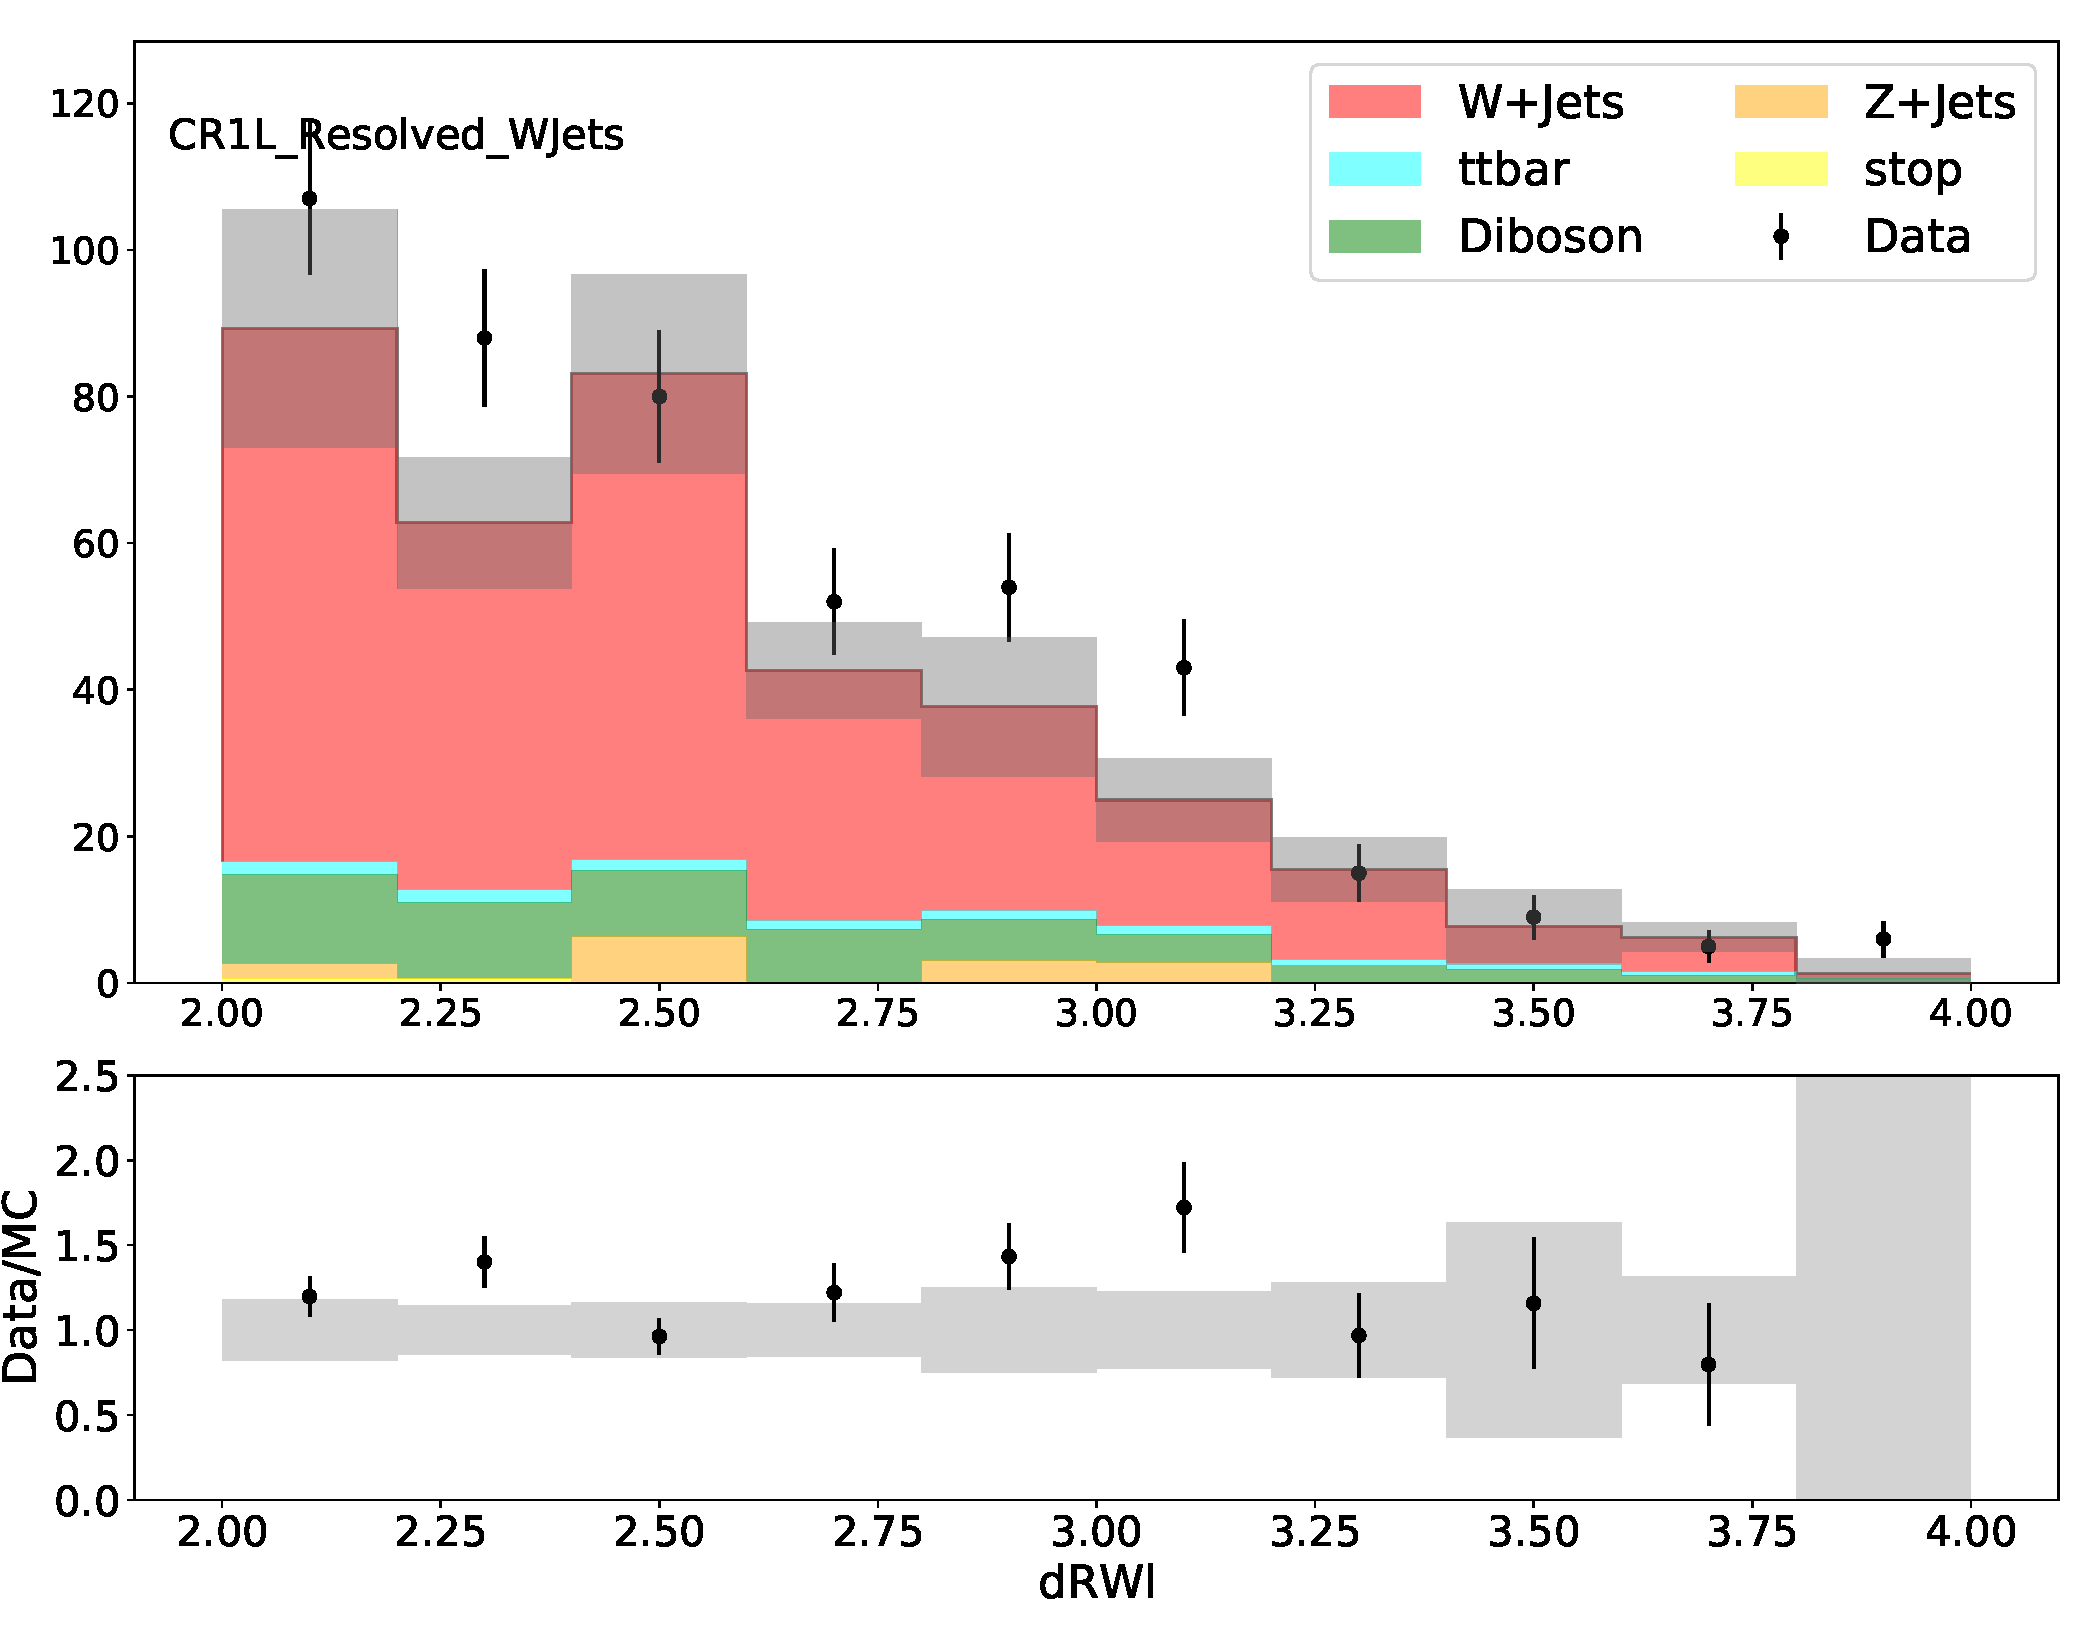
\includegraphics[width = 0.98\textwidth]{Figures/4/datamc/CR1L_Resolved_WJets/dRWl.pdf}
     \caption{\drWl}
     \end{subfigure}
     \begin{subfigure}{0.49\textwidth}
     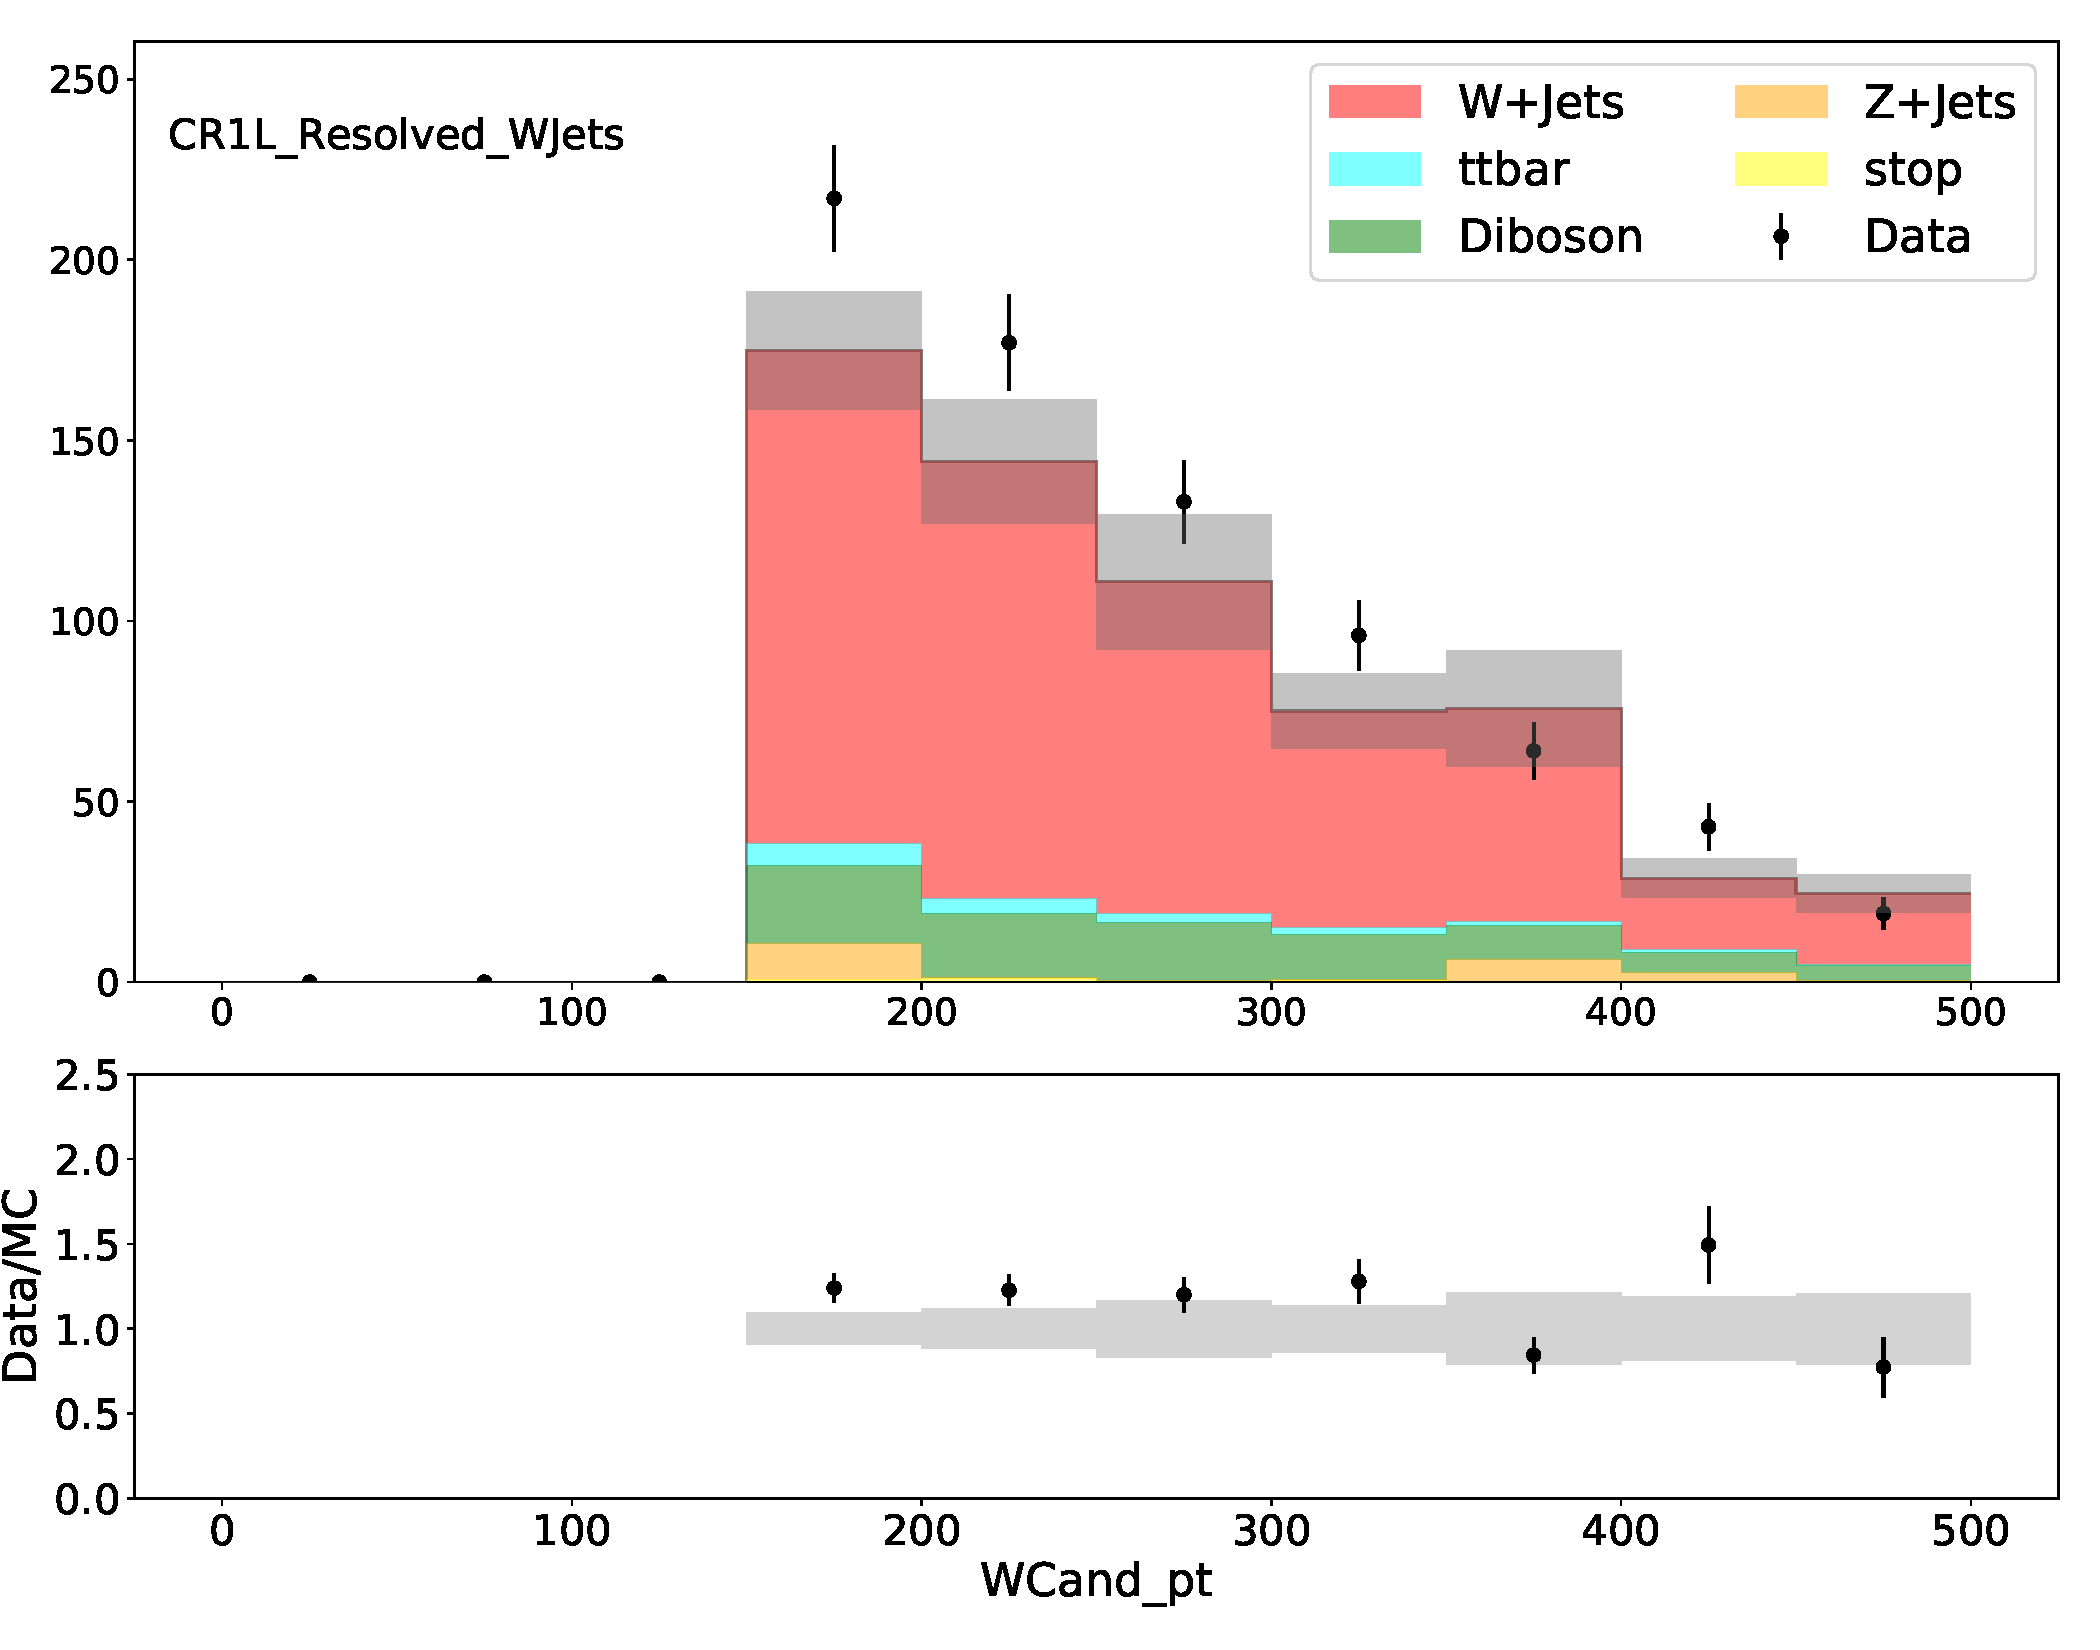
\includegraphics[width = 0.98\textwidth]{Figures/4/datamc/CR1L_Resolved_WJets/WCand_pt.pdf}
     \caption{\Wcandpt}
     \end{subfigure}
     \begin{subfigure}{0.49\textwidth}
     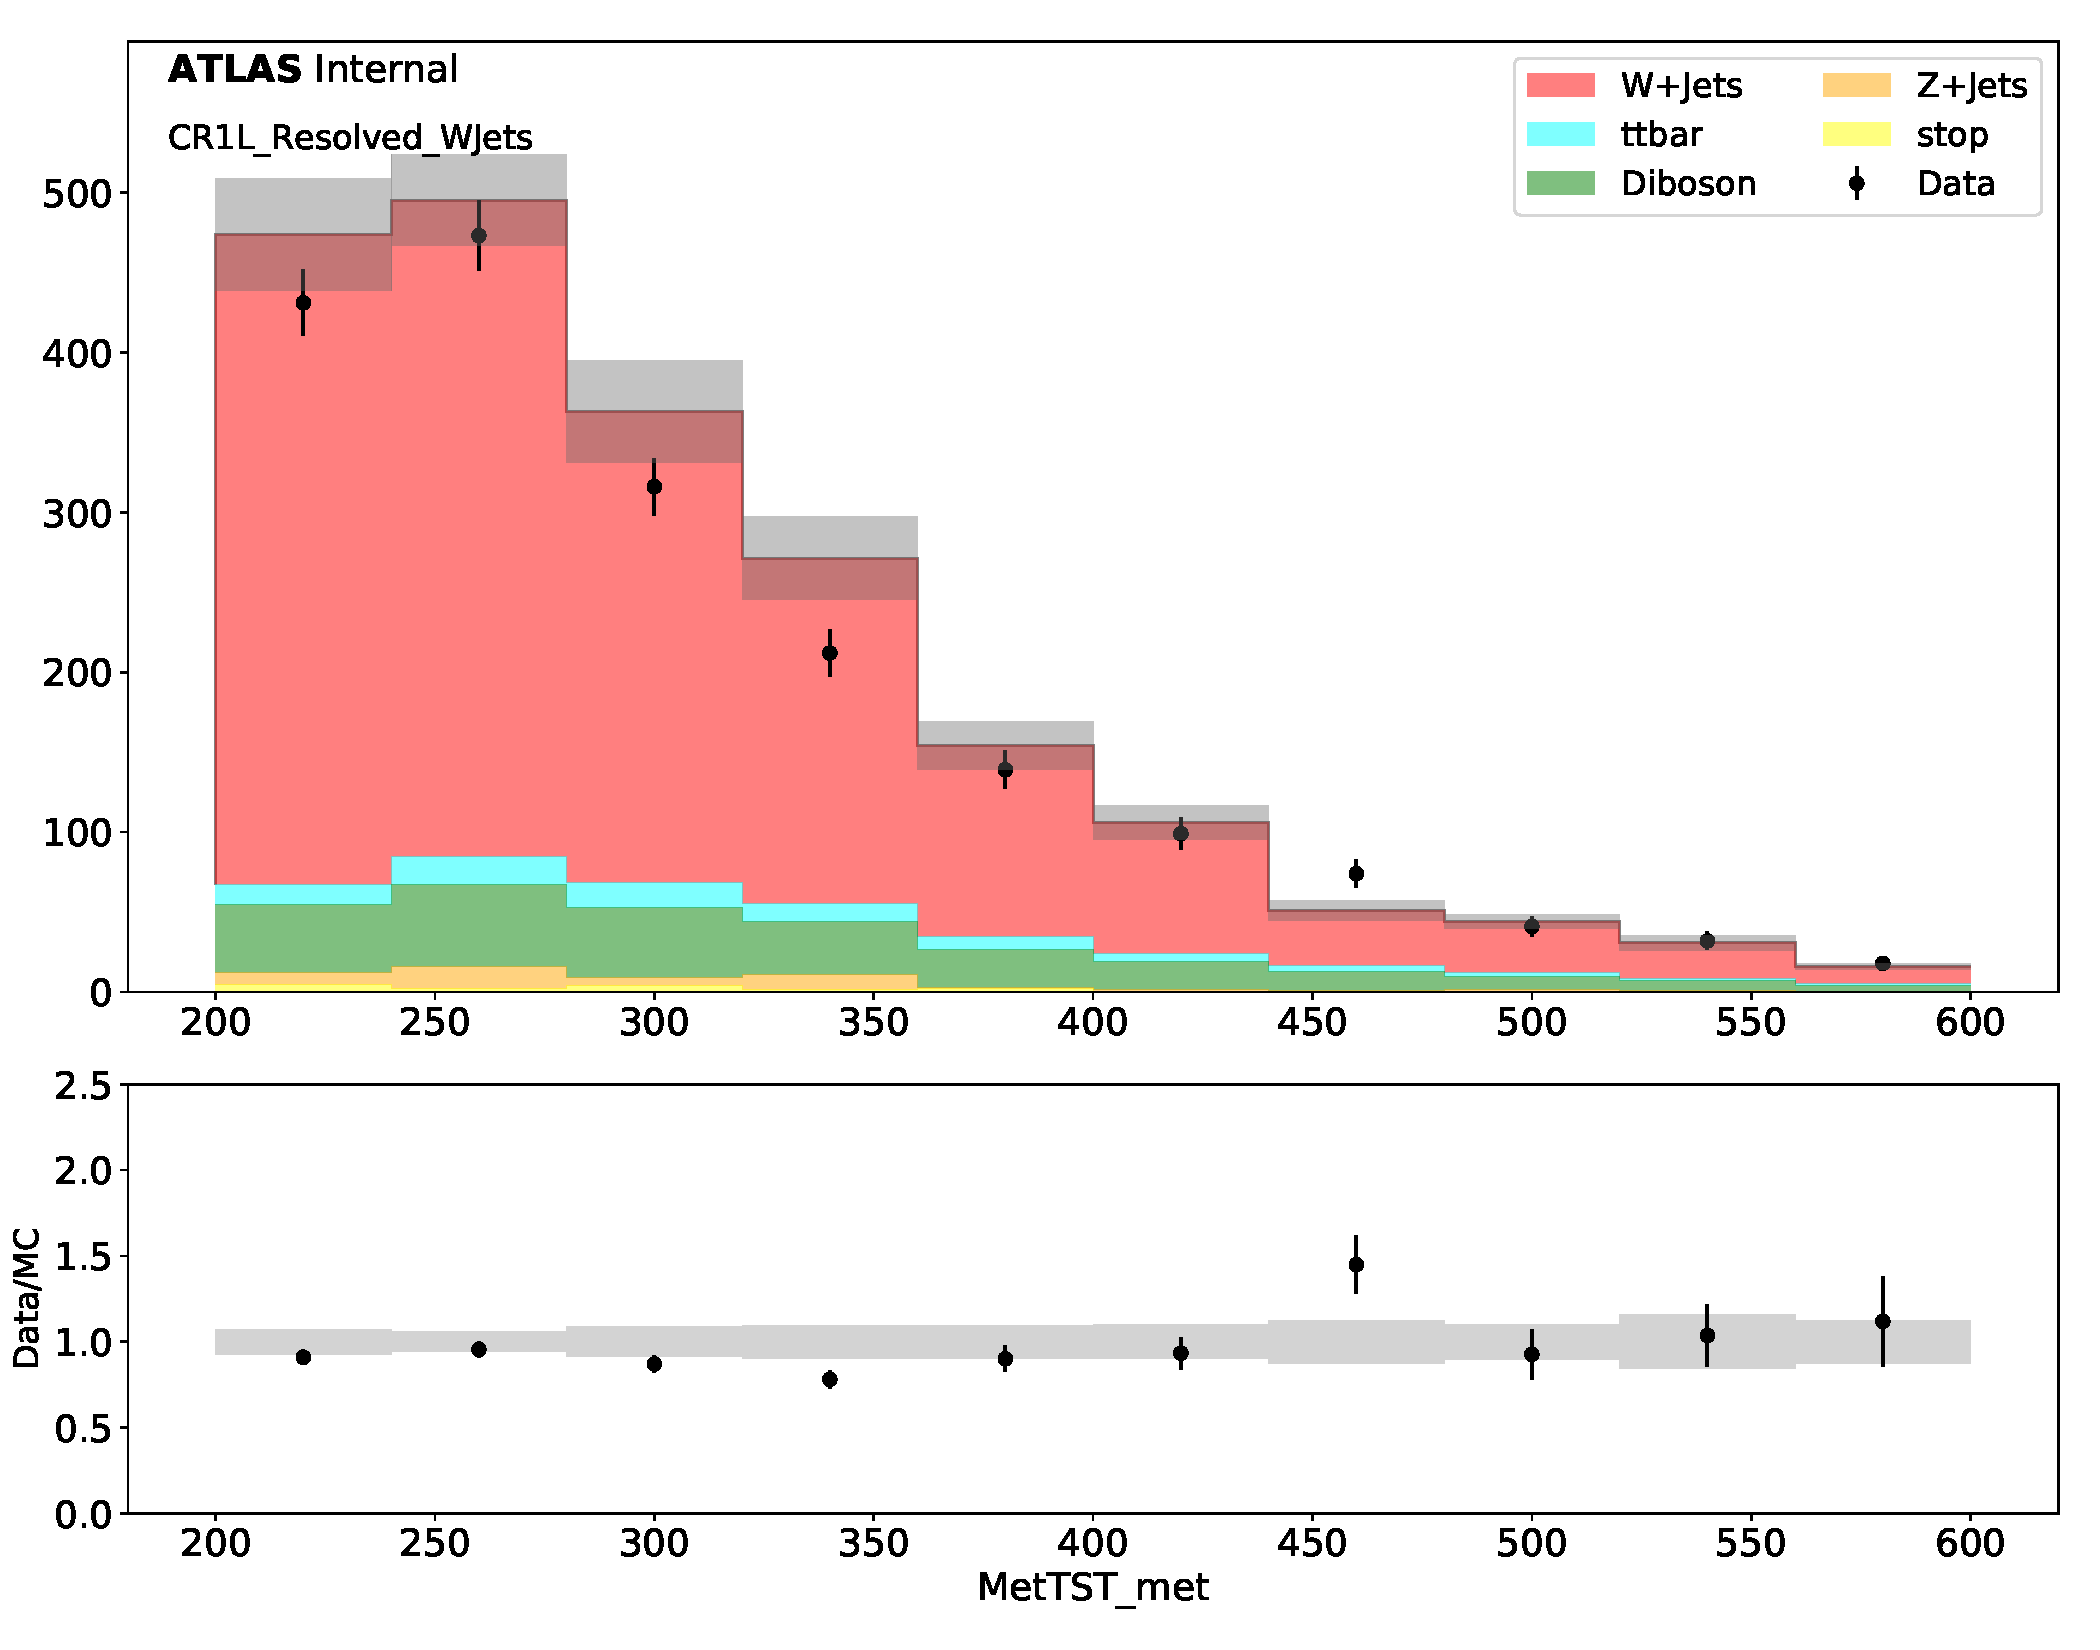
\includegraphics[width = 0.98\textwidth]{Figures/4/datamc/CR1L_Resolved_WJets/MetTST_met.pdf}
     \caption{\met}
     \end{subfigure}

     \caption{Data-MC comparisons in the \resolved \wjets control region}
     \label{fig:Data_MC_CRdR_resolved}
  \end{figure}
